\begin{savequote}[75mm]
   If I model a phenomenon accurately, does that mean I understand it? Or might it be simple coincidence, or an artifact
   of the technique? Of course, as an ardent simulationist, I myself put much faith in Engine-modeling.
\qauthor{Edward Mallory, The Difference Engine by William Gibson and Bruce Sterling}
\end{savequote}

\chapter{Wyniki}


%The following two sections describe
%different non-linear evolution of streaming instability in quasi-global setup
%with reference to similar case shown by JY07.

\section{Symulacje dwuwymiarowe}
Poniżej przedstawiono opis wyników uzyskanych dla symulacji w~przypadku
dwuwymiarowym. Ich celem, w~połączeniu z~liniową analizą stabilności, była
weryfikacja zaimplementowanych metod oraz poprawności przyjętego modelu. Każdy z
przedstawionych wyników można porównać do analogicznych eksperymentów
numerycznych z~pracy JY07~\cite{JY07}. Pomimo istotnych różnic w~użytych
metodach (JY stosowali kod wysokiego rzędu -- PENCIL, a także traktowali pył
jako cząstki materialne, a nie płyn), wyniki we wszystkich przypadkach wykazują
zgodność ilościową i~jakościową.

\subsection{Luźno związane ,,kamienie''}% ($a=50\,\textrm{cm}$, $\tau_s\approx
%1.2$)\label{marg_boulders}}

\begin{figure*}
   \centering
   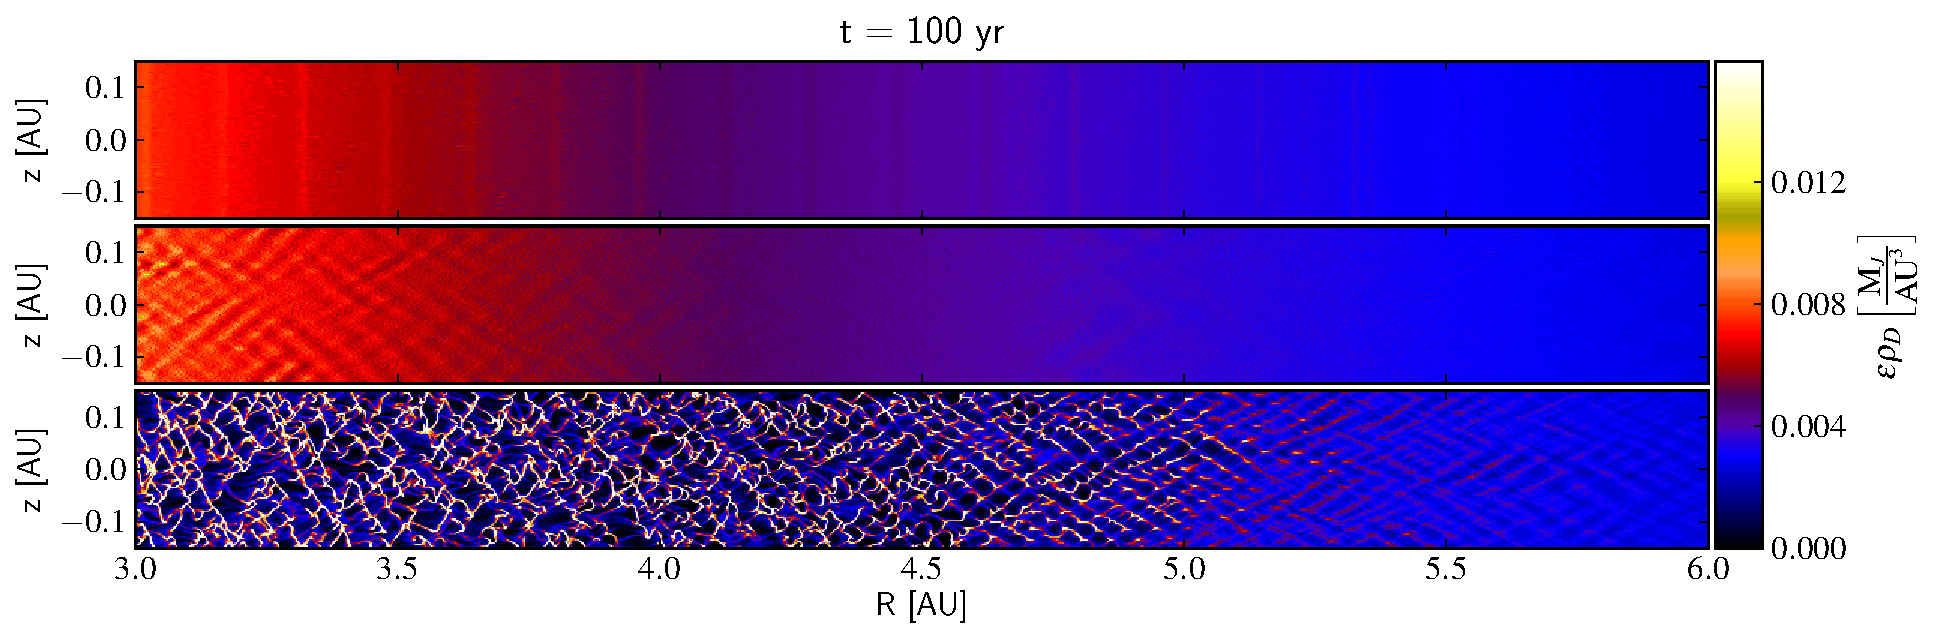
\includegraphics[width=0.99\linewidth]{figures/fig1a}
   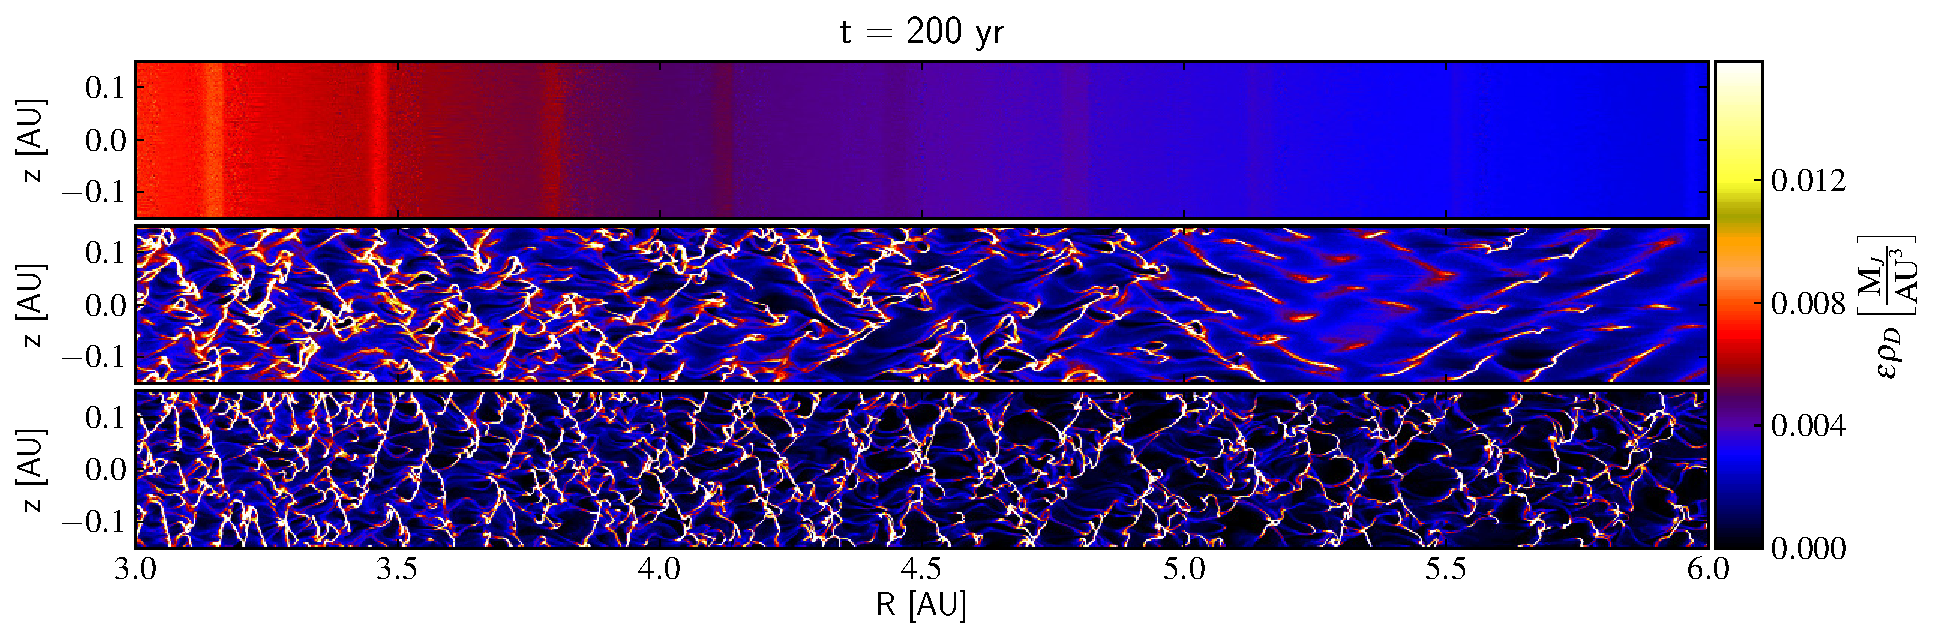
\includegraphics[width=0.99\linewidth]{figures/fig1b}
   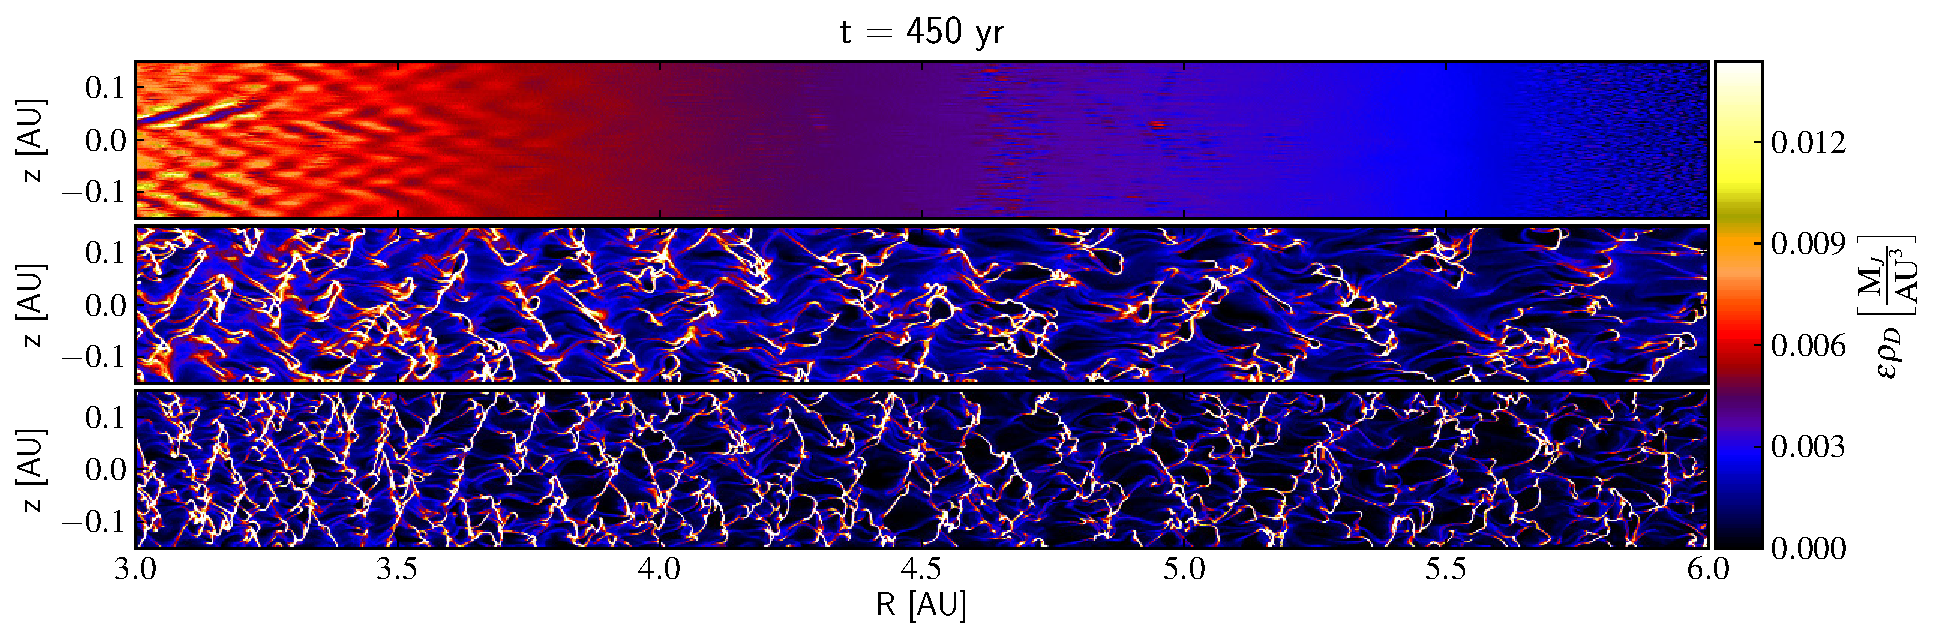
\includegraphics[width=0.99\linewidth]{figures/fig1c}
   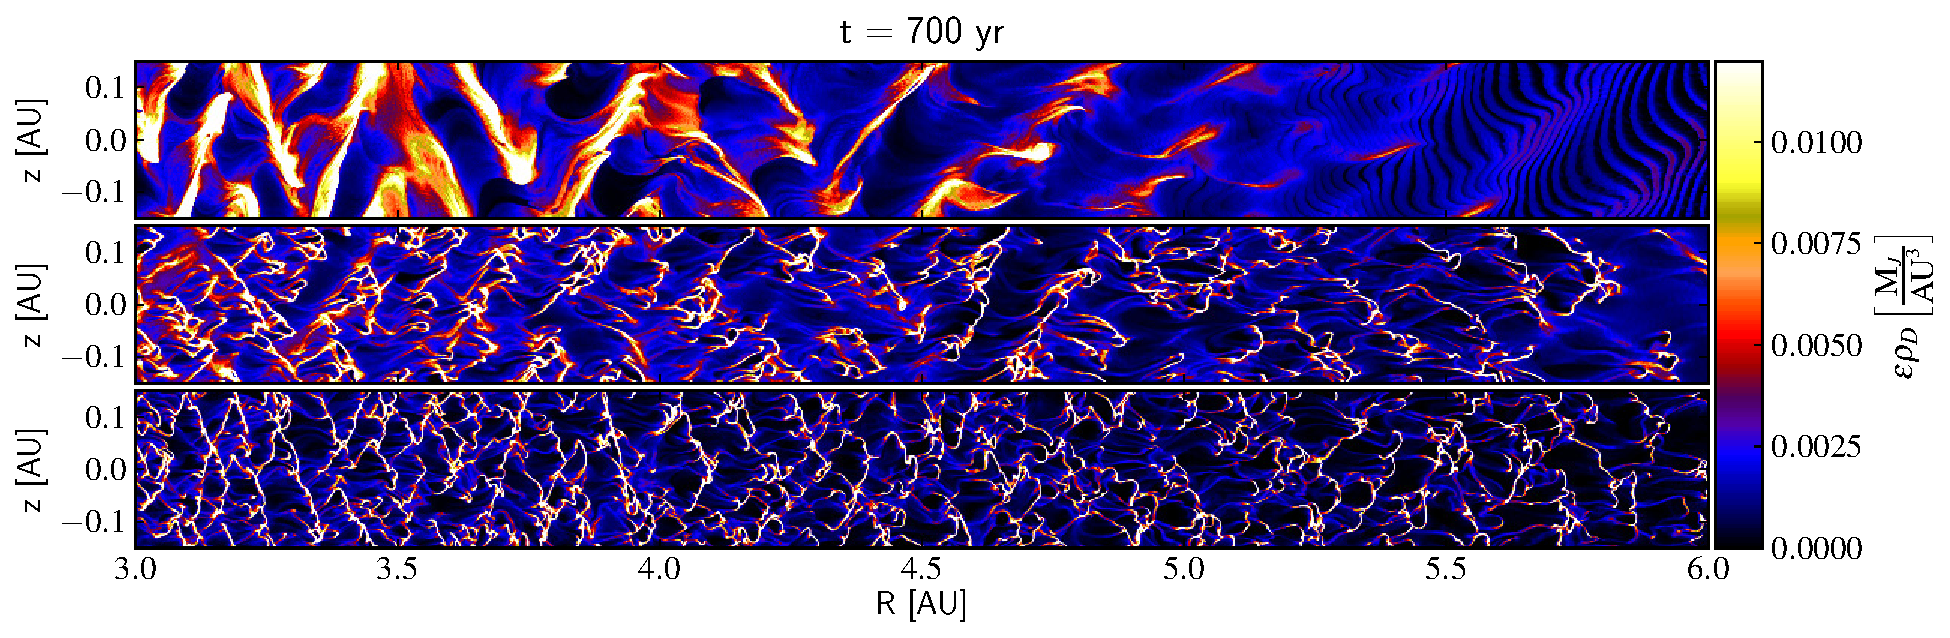
\includegraphics[width=0.99\linewidth]{figures/fig1d}
   \caption{Migawki gęstości pyłu dla symulacji z~$50$~cm ziarnami pyłu
      dla czasu $100$, $200$, $450$ oraz $700$~lat odpowiednio dla lewego
      górnego, prawego górnego, dolnego lewego i~dolnego prawego panelu.
      Każdy z~paneli jest podzielony na trzy części różniące się początkowym 
      $\epsilon = 0.2, 1, 2.0$ odpowiednio dla górnego (BAh), środkowego (BB) i
      dolnego (BC) podpanelu.}
   \label{fig1}
\end{figure*}
%

Niestabilność strumieniowa tworzy najbardziej prominentne struktury pyłu dla
cząstek pyłu o $\tau_s \sim 1$, czyli dla cząstek odsprzęgających się od
dynamiki gazu.
Przy wybranych parametrach symulacji opisanych w~rozdziale~\ref{ch2:simpar},
bezwymiarowy parametr ,,stopping time'' jest bliski jedności dla cząstek pyłu o
rozmiarach $50\cm$ (BA, BB, BC). Początkowa liniowa faza ewolucji jest
zdominowana przez wzrost gęstości dla najbardziej niestabilnych modów i~prowadzi
do znacznego wzrostu lokalnej gęstości pyłu i~uformowania się
charakterystycznych, wydłużonych diagonalnie włókien. W~rzeczywistości są to
spłaszczone struktury rozciągające się w~kierunku współrzędnej azymutalnej. Po
osiągnięciu nasycenia i~przejścia do nieliniowej ewolucji, włókna, na skutek
dużej prędkości w~kierunku wertykalnym ulegają fragmentacji i~wzajemnie się
przenikają. Jednakże pył dalej poruszą się po charakterystycznych
,,v''--kształtnych trajektoriach, które wytworzyły się podczas liniowej fazy
ewolucji. Migawki z~czasowej ewolucji gęstości pyłu zostały przedstawione na
obrazku~\ref{fig1}. Wyraźny jest wpływ początkowego stosunku gęstości pyłu do
gęstości gazu $\epsilon$ na morfologię formujących się obłoków: zarówno ich
typowy rozmiar, jak i~kąt nachylenia względem płaszczyzny dysku. Dla $\epsilon =
1$ pył poruszą się i~formuje struktury nachylone pod kątem $45^o$, dla
pozostałych przypadków $\epsilon=0.2, 2.0$ kąt nachylenia jest dużo większy,
przez co formujące się struktury są rozciągnięte w~kierunku \emph{z}. We
wszystkich wypadkach niestabilność strumieniowa prowadzi do lokalnego wzrostu
gęstości o prawie 2 rzędy wielkości.  Ze względu na swoją gęstość

\subsection{Mocno sprzężony ,,żwir''}
%($a=10\,\textrm{cm}$, $\tau_s\approx 0.24$)
%\label{tight_boulders}}
\begin{figure*}
   \centering
   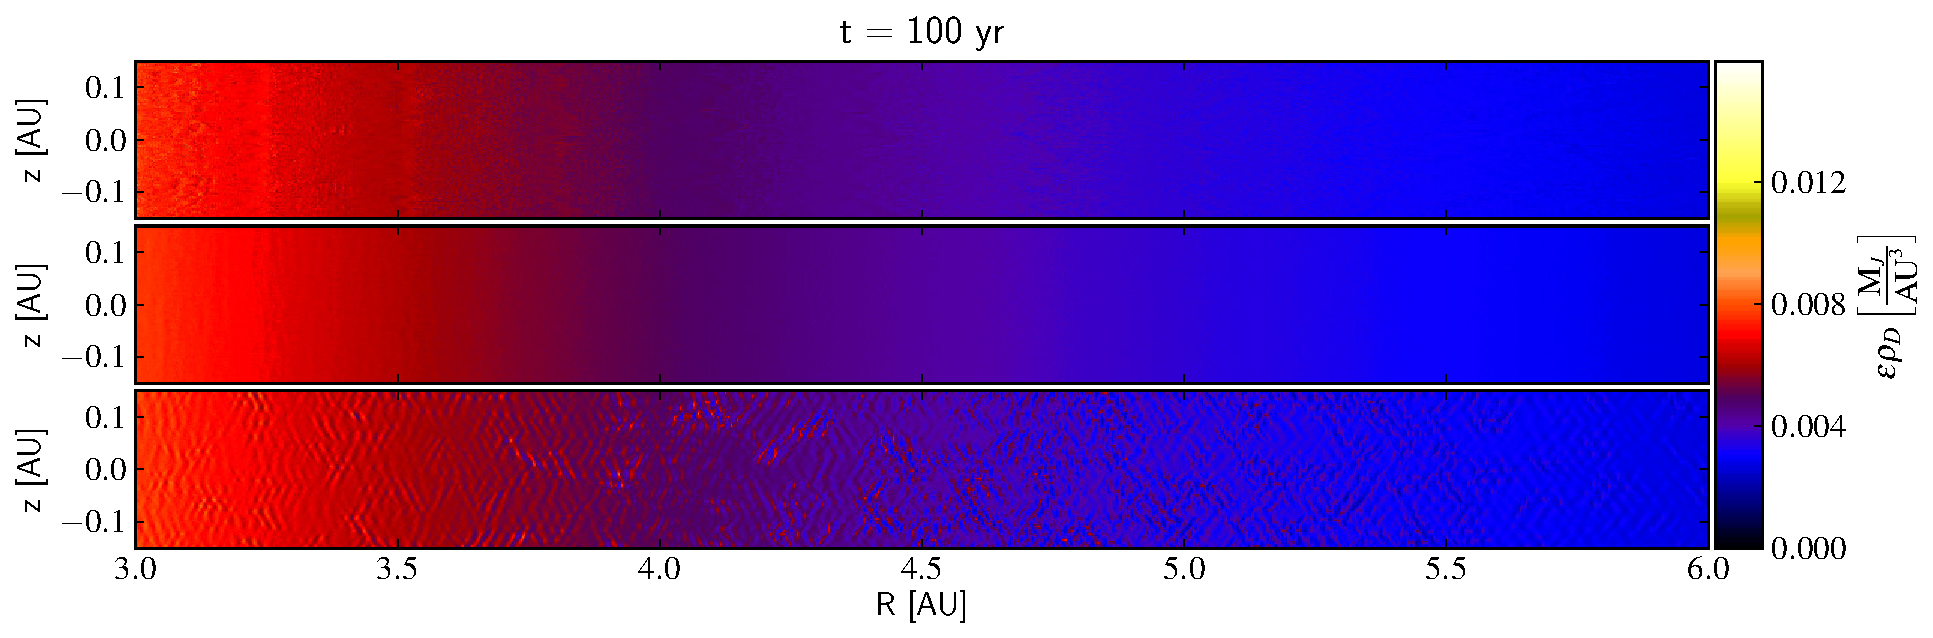
\includegraphics[width=0.99\linewidth]{figures/fig2a}
   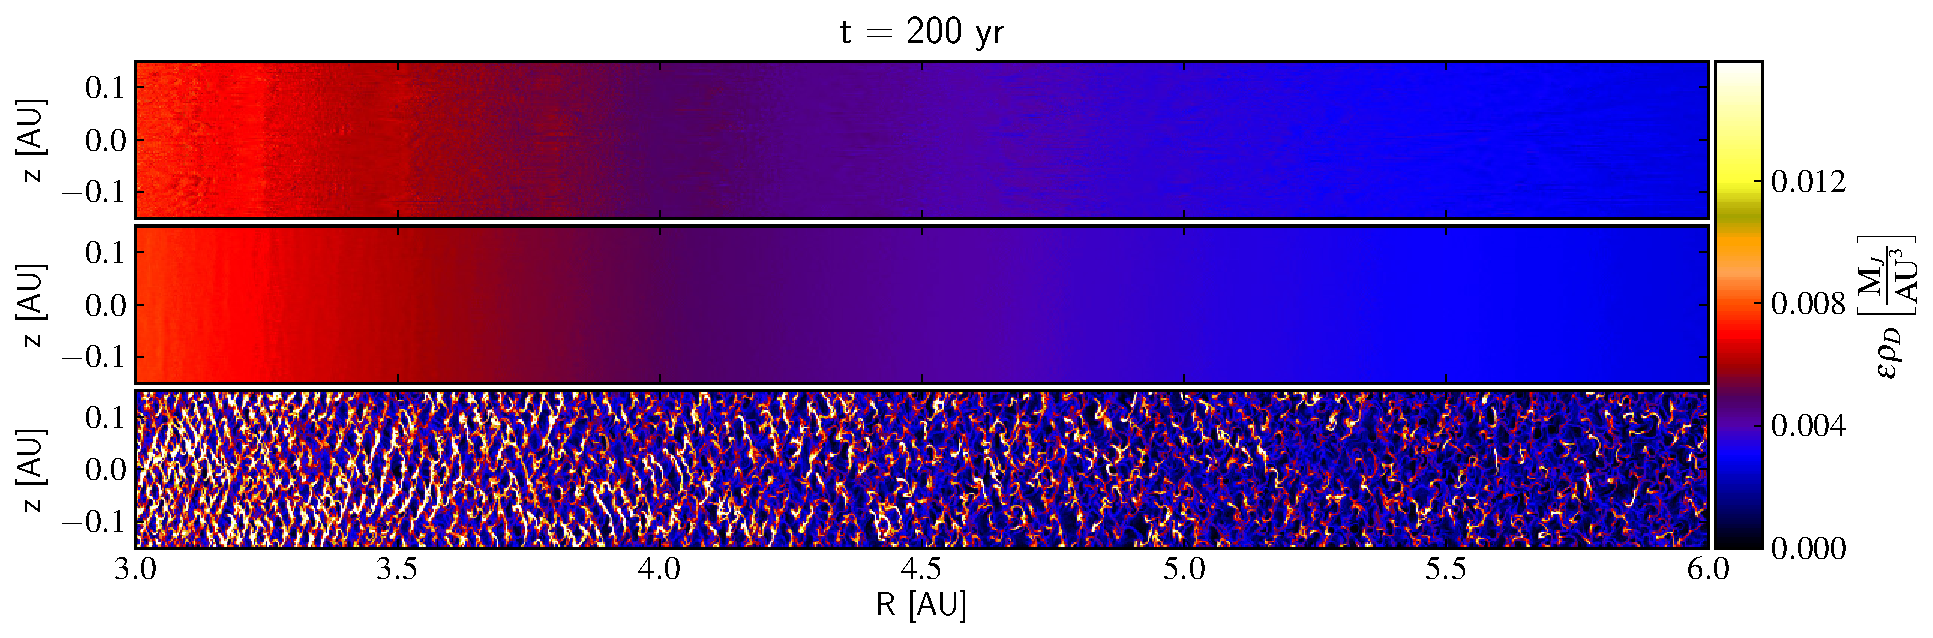
\includegraphics[width=0.99\linewidth]{figures/fig2b}
   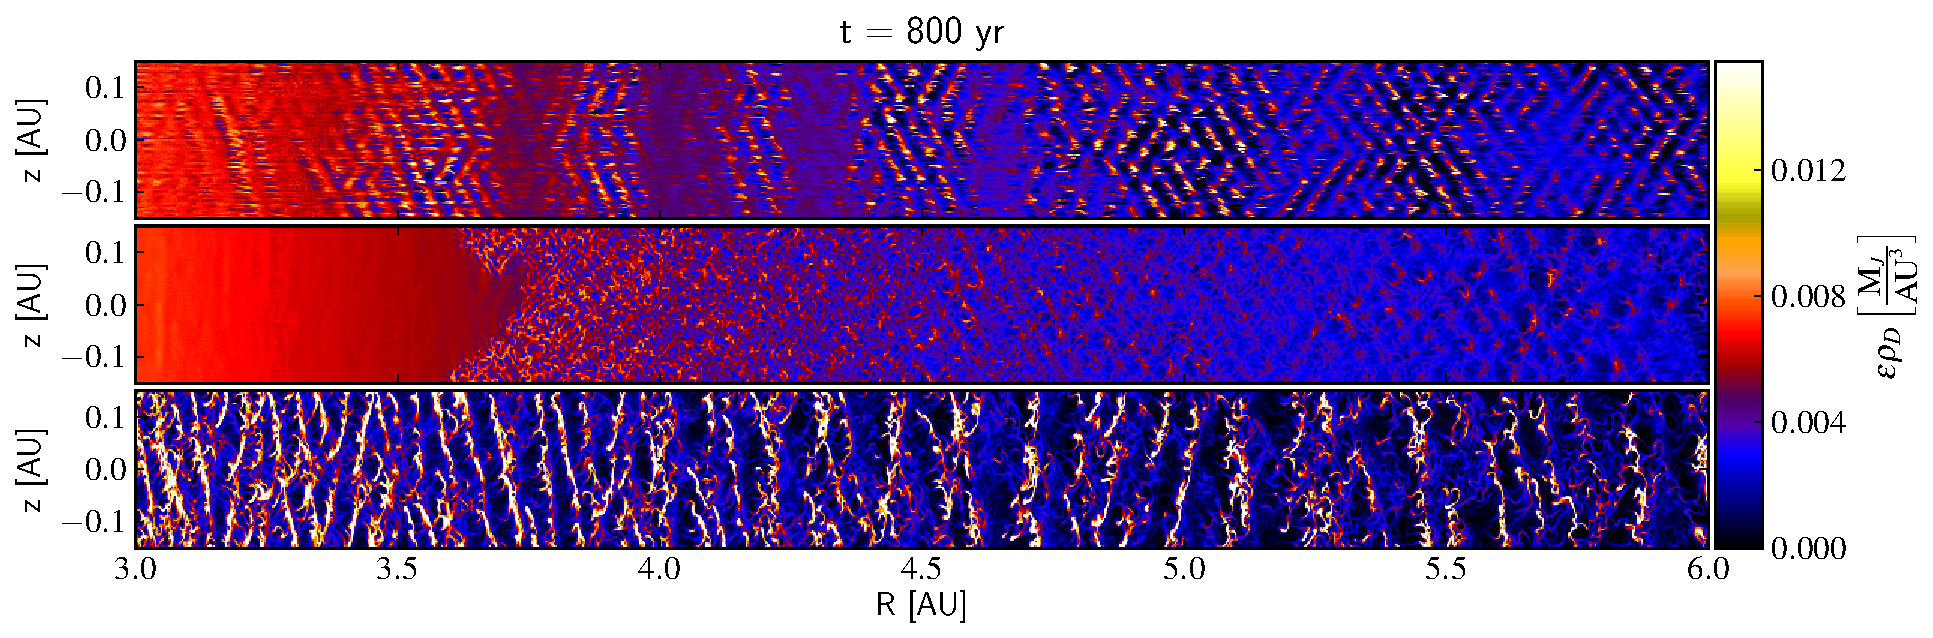
\includegraphics[width=0.99\linewidth]{figures/fig2c}
   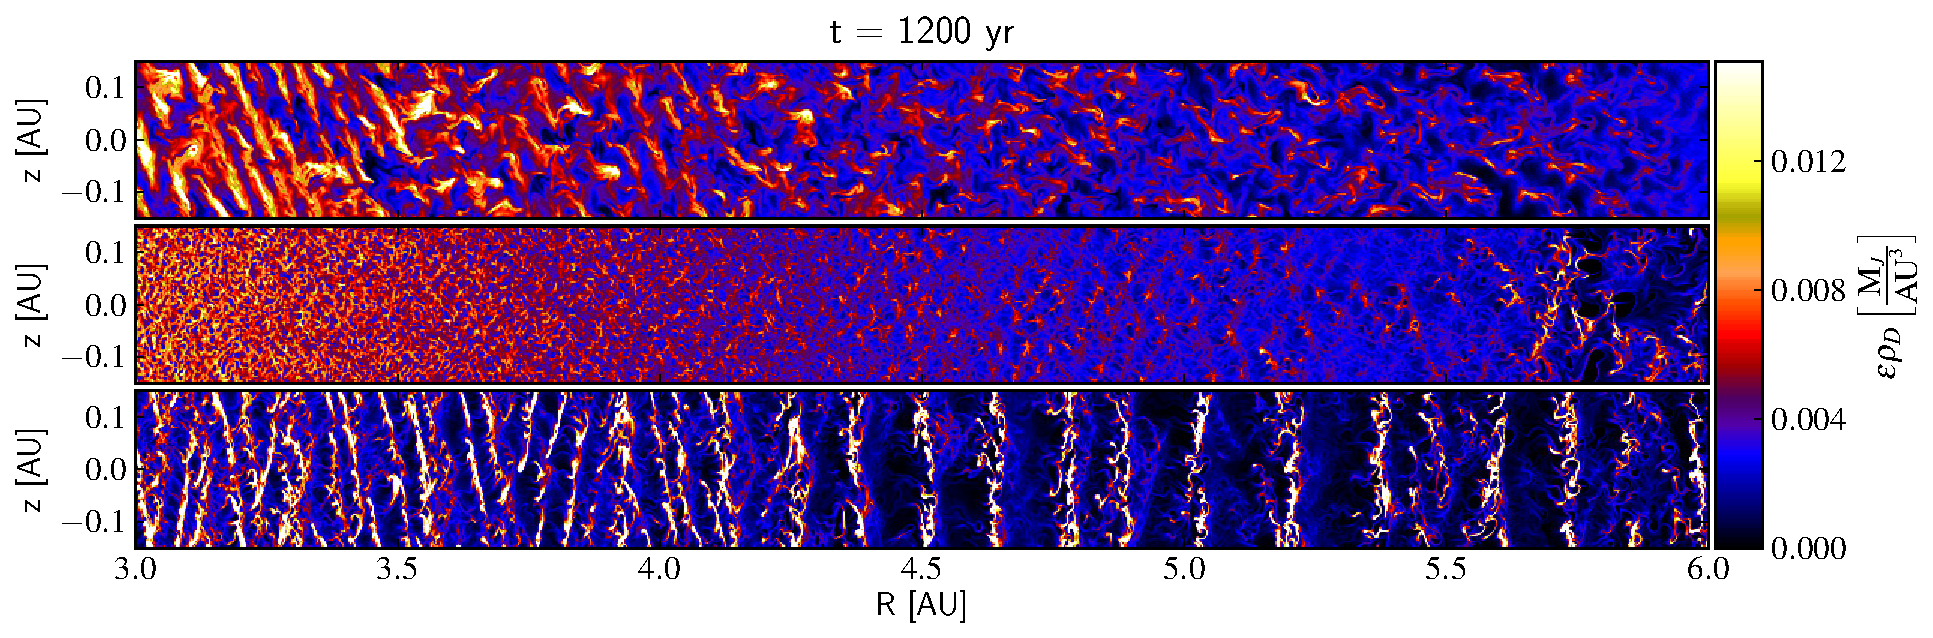
\includegraphics[width=0.99\linewidth]{figures/fig2d}
   \caption{Migawki gęstości pyłu dla symulacji z~$10$~cm ziarnami pyłu
      dla czasu $100$, $200$, $800$ oraz $1200$~lat odpowiednio dla lewego
      górnego, prawego górnego, dolnego lewego i~dolnego prawego panelu.
      Każdy z~paneli jest podzielony na trzy części różniące się początkowym 
      $\epsilon = 0.2, 1, 2.0$ odpowiednio dla górnego (AA), środkowego (AB) i
      dolnego (AC) podpanelu.}
   \label{fig2}
\end{figure*}
Czasowy przebieg symulacji dla silnie sprzężonego pyłu (AA - AC) został
przedstawiony na Rysunku~\ref{fig2}. Ewolucja pyłu dla przypadku $\epsilon =
2.0$ i~$10\cm$ ziaren pyłu (AC) nie odbiega znacząco od ewolucji analogicznego
przypadku dla $50\cm$ ziaren pyłu. Liniowa faza niestabilności podczas której
pył zostaje zagęszczony dla najbardziej niestabilnych modów, prowadzi do
wytworzenia się struktur wydłużonych w~kierunku wertykalnym. Ze względu na
mniejsze tempo migracji dla sprzężonych cząstek pyłu, zagęszczenia są pochylone
w kierunku radialnym tylko w~niewielkim stopniu. Maksymalna gęstość pyłu nie
przekracza dwudziestokrotności wartości początkowej.
\par Przypadek $\epsilon = 0.2$ charakteryzuje się niskim tempem wzrostu. W
początkowej liniowej fazie wzrost lokalnej gęstości pyły prowadzi do uformowania
się charakterystycznej diagonalnej siatki zagęszczeń. Lokalne maksima gęstości
sięgają nawet stukrotnej wielokrotności gęstości początkowej. Jednakże, przejście
do fazy nieliniowej prowadzi do gwałtownego rozmycia skupisk pyłu i~osiągnięcia
quasi-stacjonarnego stanu, w~którym zagęszczenia podlegają silnej turbulencji,
zaś ich maksymalna amplituda nie przekracza jednego rzędu wielkości względem
stanu początkowego (por. Rysunek~\ref{fig4}).

\par Najciekawszym przypadkiem, zasadniczo odbiegającym od pozostałych, jest
symulacja AB ($\epsilon=1.0,\, a=10\cm$). Początkowo ewolucja przebiega w
identyczny sposób jak dla pozostałych warunków, tzn. pojawia się regularny wzór
w gęstości pyłu odpowiadający najbardziej niestabilnym długościom fal. Jednakże 
po $800$~latach w~symulacji AB (mniej więcej dwa razy szybciej w~symulacji ABh)
pojawiają się gwałtownie rozszerzające się bąble wypełnione nie wielką ilością
pyłu, które silnie koncentrują pył na swoich brzegach (por. Rysunek~\ref{fig3}). 
Znacząco wzrasta prędkość z~którą porusza się pył, po okresie kilkuset lat
silnie turbulentne ruchy propagują się na całą domenę obliczeniową. Ta
specyficzna ewolucja niestabilności strumieniowej jest spowodowana odmiennym
przebiegiem liniowego tempa wzrostu niestabilności (patrz Rysunek~\ref{fig2b})
Dla ustalonych parametrów fizycznych AB tempo wzrostu niestabilności $s$ wypada
w punkcie przegięcia funkcji $s(\epsilon)$. Lokalne zwiększenie $\epsilon$ o
tylko $\sim10\%$ przekłada się na dwukrotne zwiększenie tempa wzrostu. Powoduje
to, że drobne zagęszczenia lokalne osiągają nieliniową fazę ewolucji dużo
szybciej niż mniej gęste obszary.  Jest to bezpośrednim powodem obserwowanego
zjawiska, które YJ określili mianem ,,kawitacji''~\footnote{jako analog
gwałtownego pojawiania się bardzo rzadkich bąbli pyłu do nagłego przejścia z
fazy ciekłej do gazowej}.  Turbulencja w~pyle prowadzi do wytworzenia się
lokalnych zagęszczeń sięgających rząd wielkości ponad stan początkowy. Jest to
zgodne z~wynikami przedstawionymi przez JY07 (patrz Rysunek.~8 w~Ich pracy).

\begin{figure} 
\centering
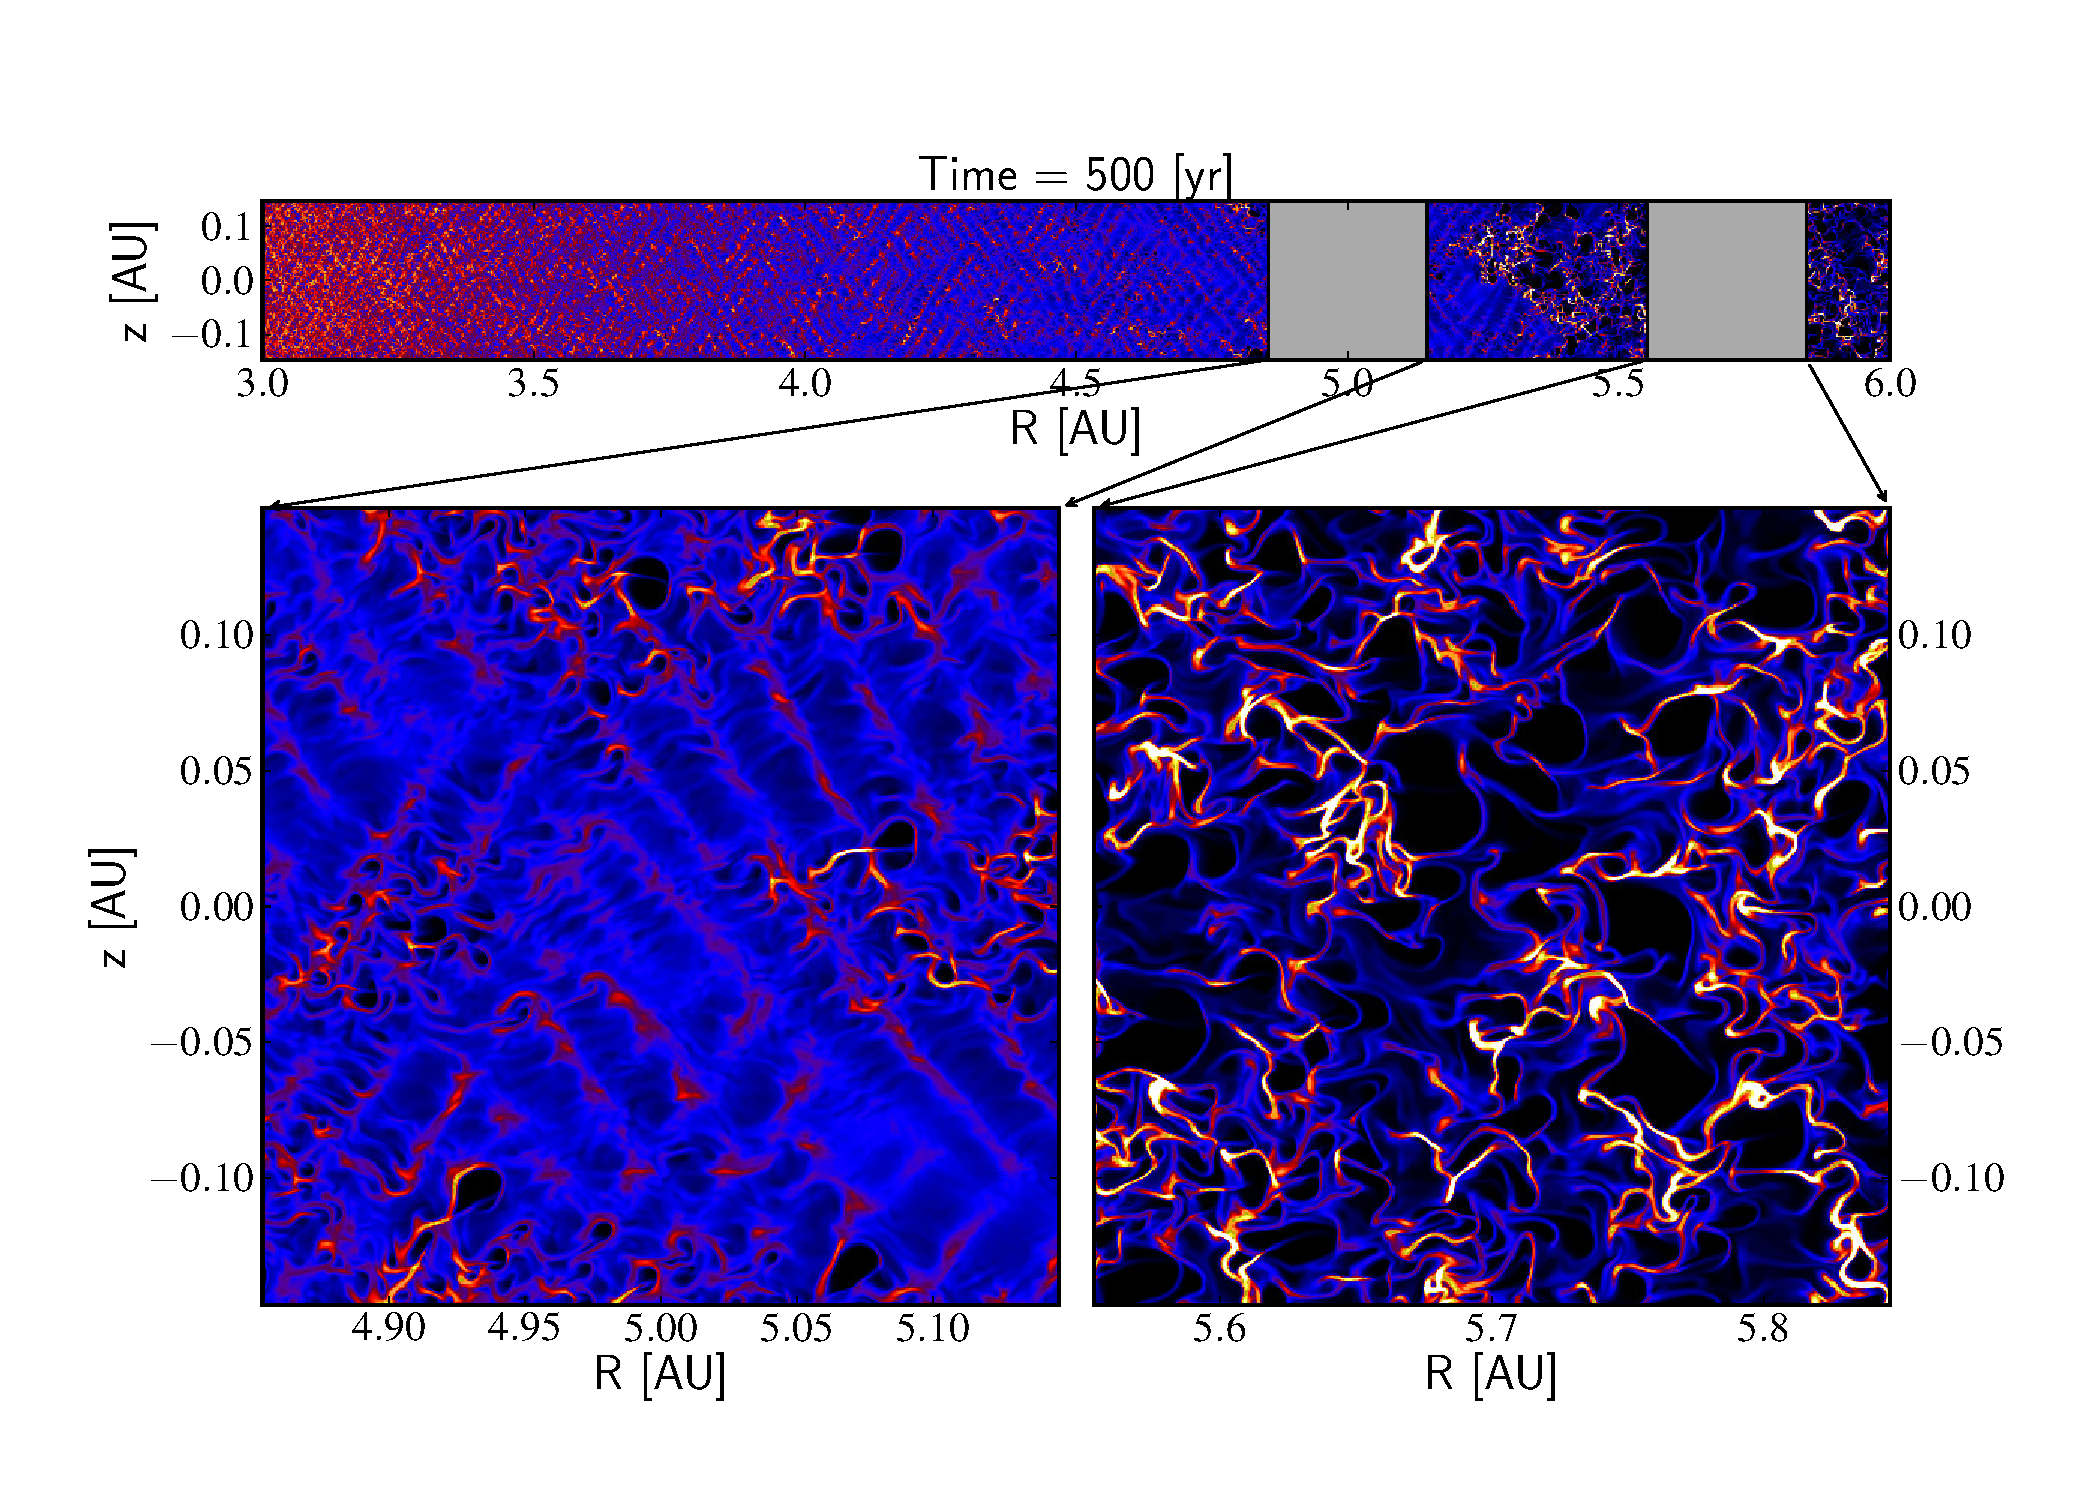
\includegraphics[width=0.98\linewidth]{figures/fig3}
\caption{Migawki gęstości gazu dla symulacji ABh pokazujące dwa ,,zbliżenia''
   obszarów gdzie: występuje pseudo-kawitacja wynikająca z~lokalnych zagęszczeń
   wytworzonych w~liniowej fazie wzrostu (lewy panel) oraz region całkowicie
   opanowany przez wybuchające bąble pustki i~silną turbulencję pyłu (prawy
   panel). Animacja przedstawiająca ewolucję symulacji ABh jest dostępna pod
   adresem \href{http://youtu.be/NoA5-TiQabQ}{http://youtu.be/NoA5-TiQabQ}.}
\label{fig3}
\end{figure}

\begin{figure}
   \centering
   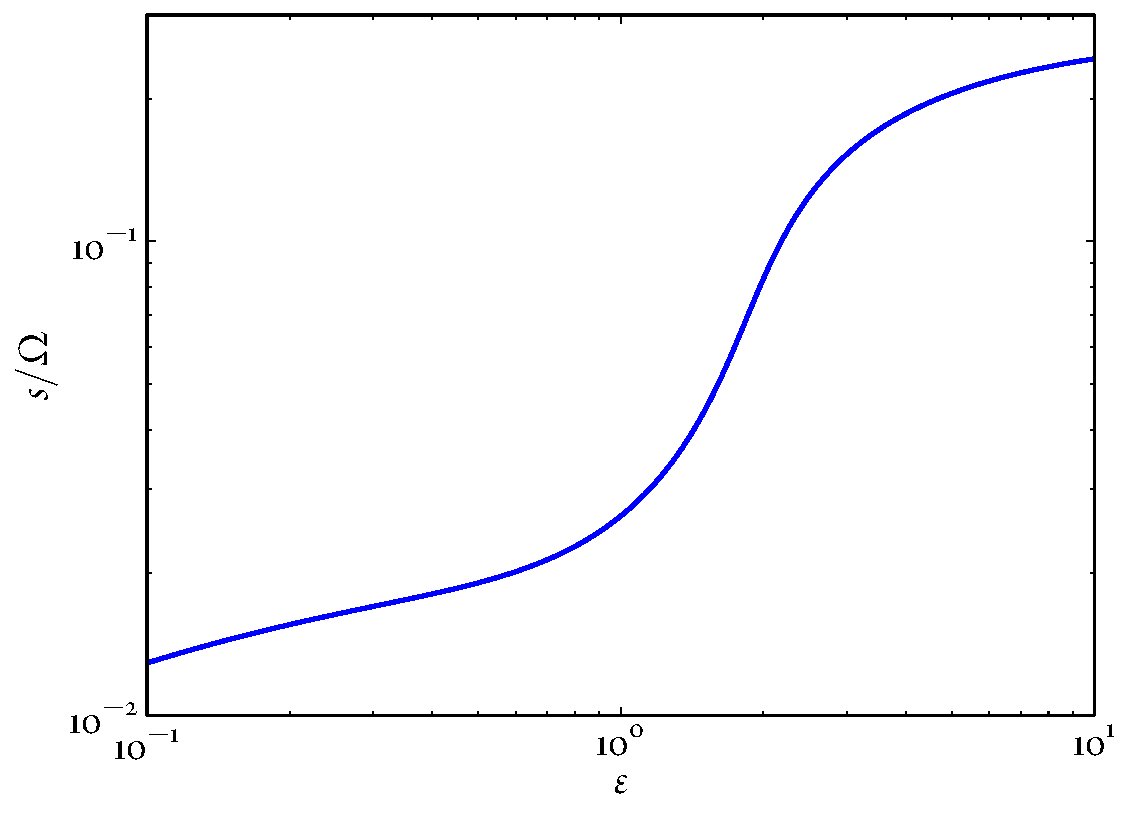
\includegraphics[width=0.5\linewidth]{figures/growthAB}
   \caption{Liniowe tempo wzrostu niestabilności strumieniowej jako funkcja
      stosunku gęstości pyłu do gęstości gazu. Pozostałe parametry niezbędne do
      rozwiązania równania~\mref{eq:disprel} zostały wzięte obszaru znajdującego
   się na lewym panelu Rysunku~\ref{fig3}.}
   %Przełamanie przebiegu funkcji dla
   %   $\epsilon\sim 1$ jest bezpośrednim powodem ,,kawitacji'' obserwowanej w
   %   symulacji AB}
   \label{fig2b}
\end{figure}


\begin{figure}
   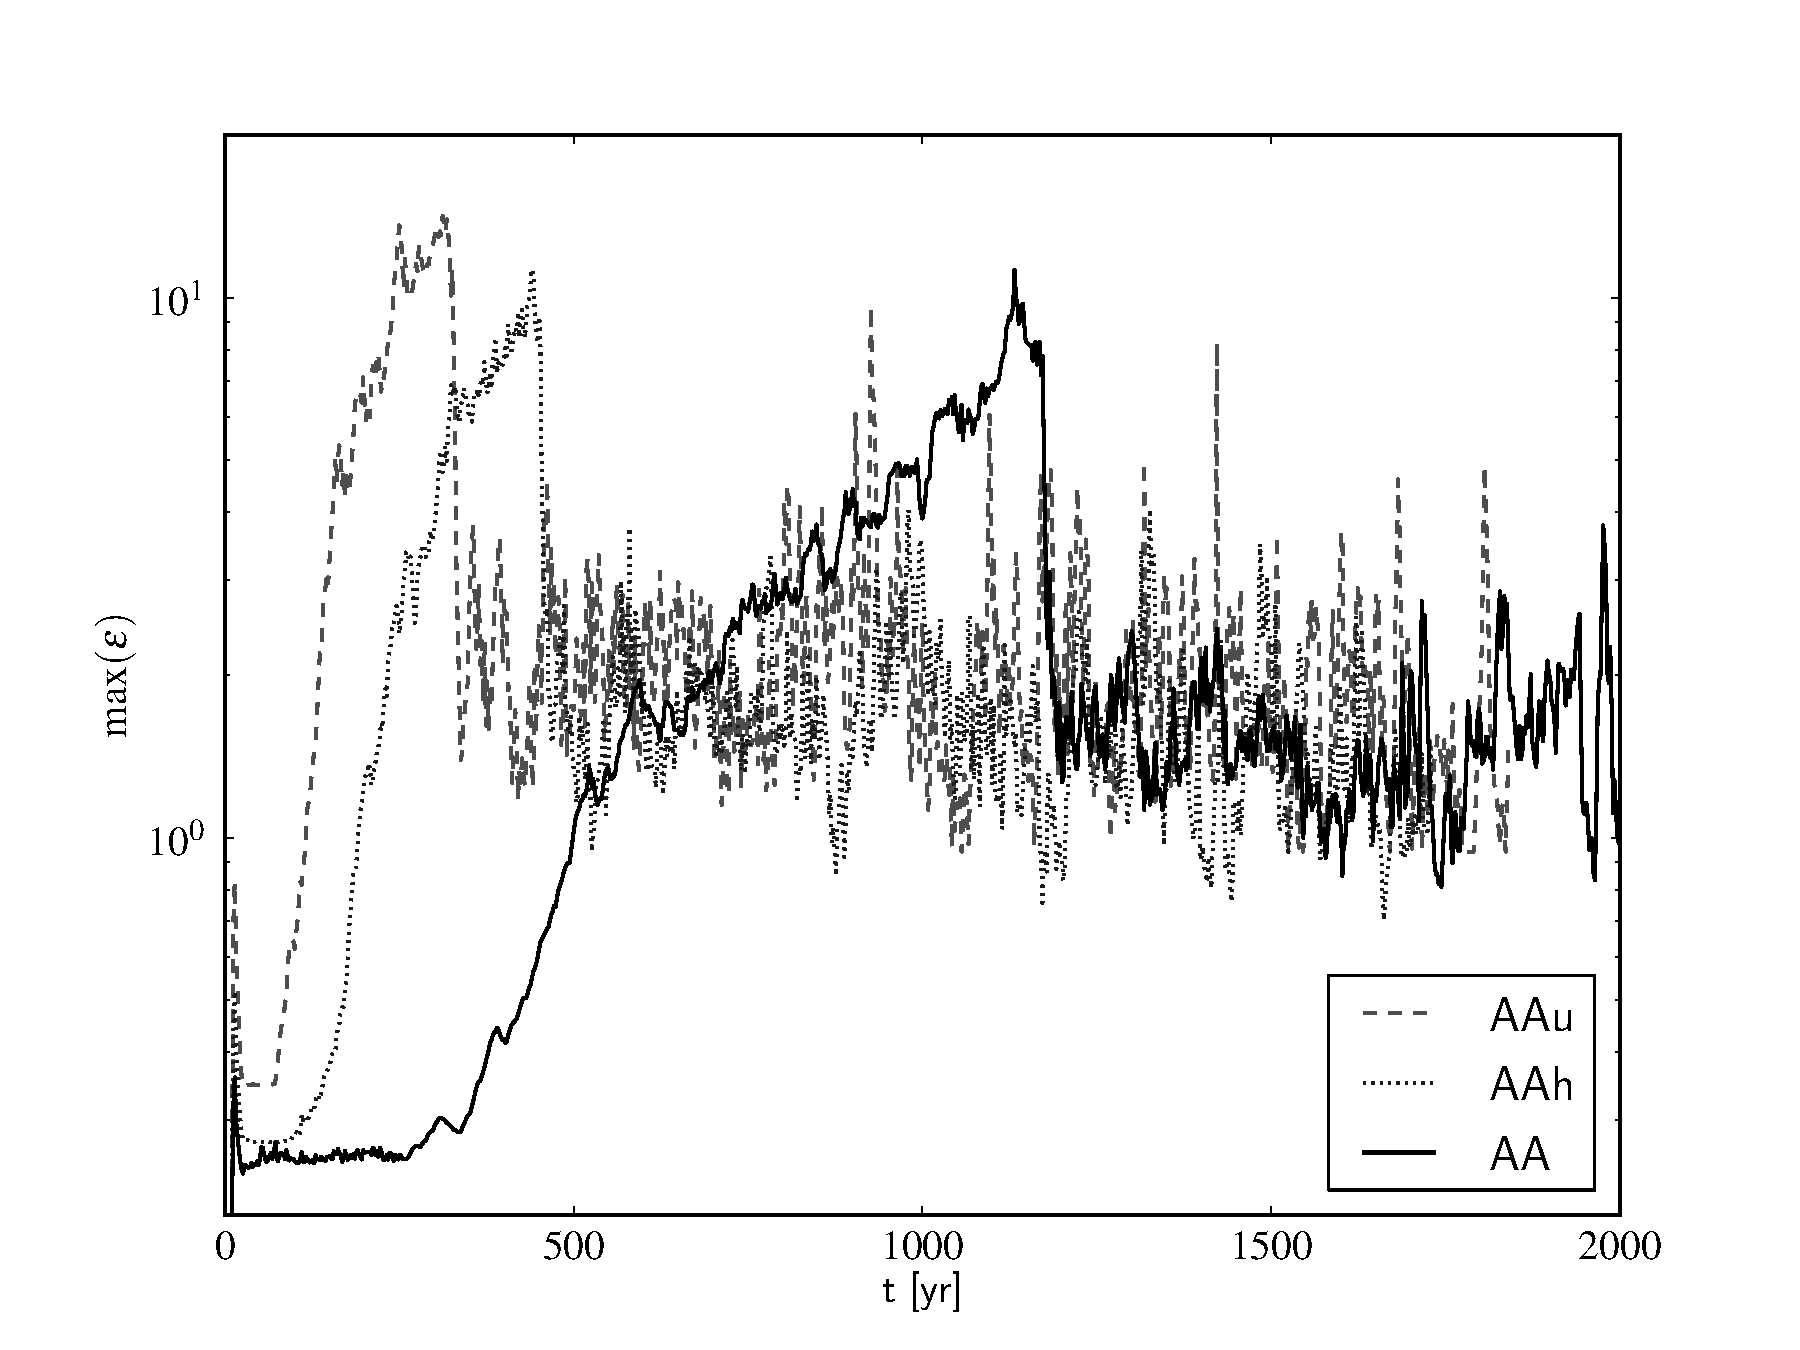
\includegraphics[width=0.98\linewidth]{figures/fig4}
   \caption{
      Maksymalne stosunek gęstości pyłu do gęstości gazu dla trzech symulacji z
      identycznymi, fizycznymi warunkami początkowymi, lecz różną
      rozdzielczością. Ewolucja niestabilności strumieniowej przebiega według
      scenariusza: (1) szybki wzrost podczas liniowej fazy ewolucji, który
      zwiększa lokalnie $\epsilon$ o dwa rzędy wielkości, (2) po
      osiągnięciu krytycznego $\epsilon\approx 10$, zagęszczenia pyłu zostają
      gwałtownie rozmyte, (3) niestabilność osiąga wysycenie, nieliniowa
      ewolucja sprowadza się do oscylacji gęstości pyłu w~postaci dużych,
      rozmytych obszarów o maksymalnej gęstości nieprzekraczającej
      dziesięciokrotności wartości początkowej. Zmiana rozdzielczości nie ma
      wpływu na powyższy scenariusz, jedynie wprowadza krótsze i~szybciej
   rosnące długości fal skracając etap (1).}

   \label{fig4}
\end{figure}
%

\section{Porównanie wyników z~liniową analizą stabilności}
\label{sec:simulation_analysis}
Aby móc porównać obserwowane tempa wzrostu niestabilności strumieniowej z
analizą przedstawioną w~rozdziale~\ref{sec:lsa} z~domeny obliczeniowej
wyodrębniono małe, kwadratowe ,,łatki'' na wybranych orbitach. Rozmiar wybranych
obszarów $(0.15^2\AU)$ pozwala traktować je w~ramach lokalnego przybliżenia
kostki ścinanej, a także umożliwia wyrażenie stałych parametrów występujących w
równaniach \mref{lin1}--\mref{lin4}) poprzez wartości średnie w~łatce.
Można zatem przyjąć, że $\bar{\rho}_g = \left<\rho_g\right>$, $\bar{\rho}_d =
\left<\rho_d\right>$ to średnie przestrzenne odpowiednio gęstości gazu i
gęstości pyłu, oraz że ich średni wzajemny stosunek to $\bar{\epsilon} =
\left<\rho_d / \rho_g\right>$. Jako Średnią częstość kątowa $\bar{\Omega}$
przyjęto częstość kątową środka łatki. Bezwymiarowa miara podkeplerowskiej
rotacji jest obliczona zgodnie ze wzorem (patrz YG05 rów.~(16) albo JY07
rów.~(1)).  Wypadku trójwymiarowych symulacji, które dokładnie zostaną opisane
w kolejnych częściach tego rozdziału, ,,łatka'' została wybrana w
płaszczyźnie {\it r-z} dla $\varphi = \varphi_\textrm{max} / 2$.
%
\begin{equation}
   \bar{\eta} = -\frac{c_s^2\left<\partial_R \left<\rho_g\right>_z\right>_R}
      {2\bar{\rho}_g\bar{\Omega}^2 R},
   \label{eq:meaneta}
\end{equation}
%
W~równaniu~\mref{eq:meaneta} średnia z~gęstości gazu jest liczona najpierw w
kierunku wertykalnym, a następnie jest obliczana średnia z~radialnej pochodnej 
$\left<\partial_R \rho_g\right>$. Wyrażenie na średni ,,stopping time'' zostało
wyprowadzone z~równania~\mref{eq:tauf}
\begin{equation}
   \bar{\tau}_f = \rho_\bullet a / \left(\bar{\rho}_g \sqrt{c_s^2 +
   \left<\left|\mathbf{u} - \mathbf{v}\right|^2\right>} \right).
\end{equation}
%
Dla spójności średnie prędkości gazu i~pyłu $\bar{\mathbf{u}},
\bar{\mathbf{w}}$ również są brane jako średnie wartości
$\left<\mathbf{u}\right>, \left<\mathbf{w}\right>$ zamiast obliczania ich przy
pomocy równań~\mref{eq:w0}-\mref{eq:u0} wynikających z~założenia dodatkowego
członu w~równaniach, niezbędnego w~przybliżeniu kostki ścinanej. 
Należy zauważyć, że wartości $\left<\mathbf{u}\right>, \left<\mathbf{w}\right>$,
osiągnięte w~sposób naturalny w~trakcie trwania symulacji, nie różnią się od
wartości analitycznych o więcej niż $10\%$.
\par Aby określić liniowe tempo wzrostu dla wzbudzanych modów niestabilności
rozkład gęstości i~prędkości poszczególnych płynów został przekształcony przy
pomocy transformaty Fouriera, tak aby uzyskać informację o amplitudach
wzbudzanych fal. Analiza przebiegu czasowego zmienności amplitud dla
poszczególnych częstości pozwala wyizolować najbardziej niestabilne mody układy.
Ten etap analizy dla jednej z~łatek został przedstawiony na Rysunku~\ref{fig7}.

\begin{figure}
  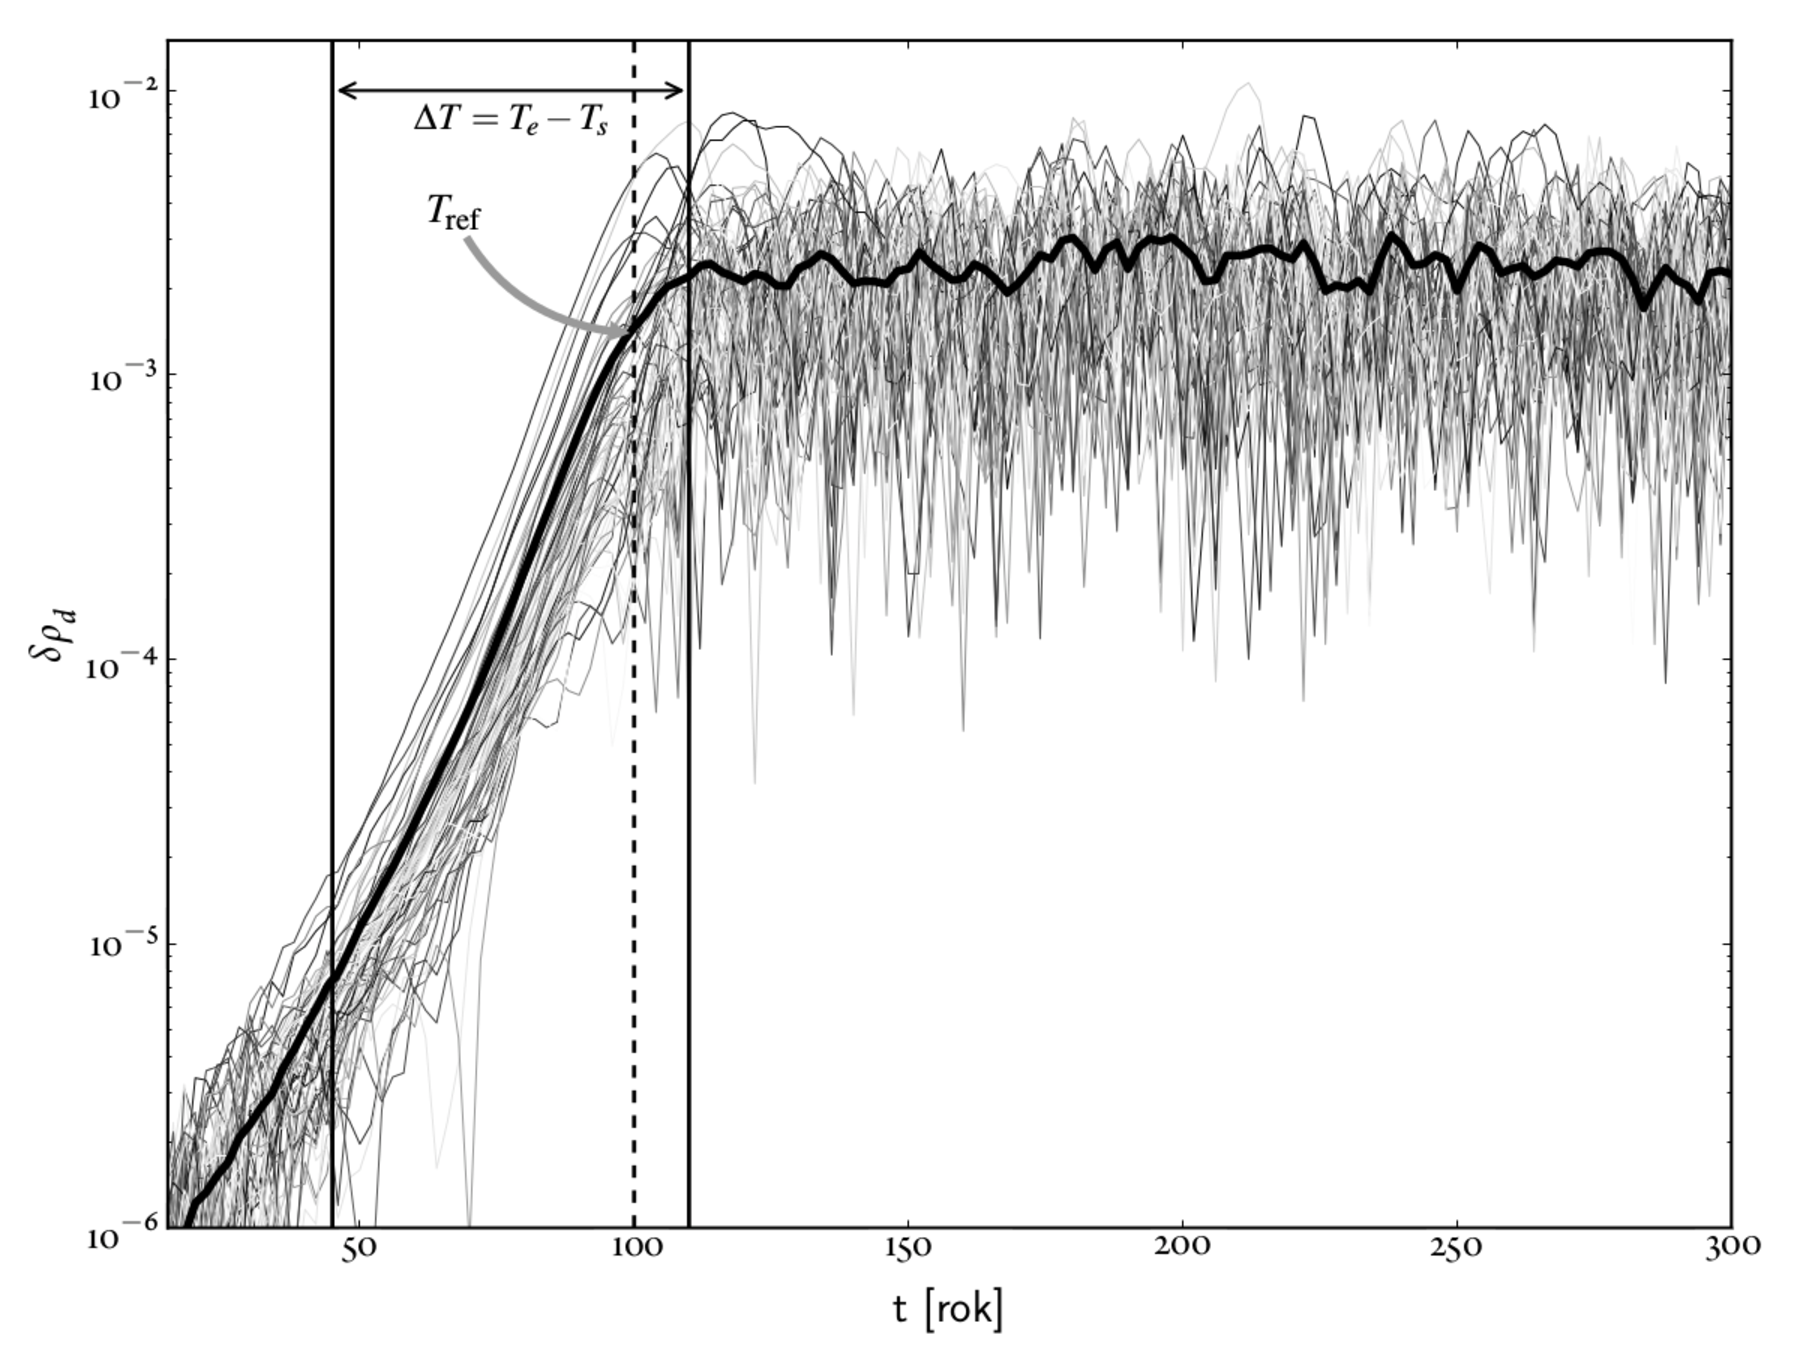
\includegraphics[width=0.98\linewidth]{figures/fig7}

  \caption{Czasowa ewolucja amplitud zaburzenia gęstości pyłu w~przestrzeni
     fourierowskiej dla łatki z~symulacji BB obejmującej obszar 
     $[2.85,3.15]\times[-0.15,0.15]~\AU^2$. Każda cienka, szara linia
     reprezentuje amplitudę dla wybranej pary liczb falowych $k_x, k_z$.
     $\Delta T = T_e - T_s$ to odcinek czasu dla którego do modów jest
     dopasowywane równanie~\mref{eq:fit}. $T_{\textrm{ref}}$ to punkt
     odniesienia dla którego identyfikowane są dominujące mody na podstawie
     wartości maksymalnej amplitud. Gruba, czarna linia pokazuje uśredniony
     przebieg zmienności dla modów, których amplituda dla $t = T_{\textrm{ref}}$
     jest większa niż $10^{-4}$.} 
   \label{fig7} 
\end{figure}

Dla każdego z~badanych obszarów określono czas $T_s$ dla którego część modów
zaczyna wyłaniać się z~szumu i~rozpoczyna fazę liniowego wzrostu. Na
podobnej zasadzie wyznaczono czas $T_e$, dla którego następuje wysycenie
wzrostu. Następnie do wszystkich modów na przedziale $\Delta T = T_e - T_s$
zostaje dopasowana funkcja
%
\begin{equation}
   f(t) = A\exp\left(-s t\right).
   \label{eq:fit}
\end{equation}
%
Powyższa procedura pozawala na określenie tempa wzrostu w~funkcji liczb falowych
$s(k_x, k_z)$ dla wszystkich modów podczas ich liniowego wzrostu. Mody rosnące
najszybciej są określane poprzez znalezienie modów o najwyższej amplitudzie w
wybranym momencie czasu $T_{\textrm{ref}} \lesssim T_e$, tuż przed ich
saturacją. Żadnej z~wielkości: $T_s$, $T_e$, $T_{\textrm{ref}}$ nie da się
określić w~jednoznaczny sposób. Dla każdej łatki z~osobna były one dobierane
arbitralnie na podstawie wizualnej oceny przebiegu dużej ilości modów (patrz
rysunek~\ref{fig7}).  Po określeniu ich tempa wzrostu $s(k_x, k_z)$ jest ono
porównywane z~tempem wzrostu $s_0(k_x, k_z)$ wynikającym bezpośrednio z~liniowej
analizy dla średnich wielkości płynowych w~łatce.

\par Rysunek~\ref{fig8} pokazuje czasową ewolucję amplitud zaburzenia gęstości
pyłu dla 3 najszybciej rosnących modów, wraz z~dopasowaną funkcją~\mref{eq:fit}
i tempem wzrostu wynikającym z~liniowej analizy dla symulacji BB3d, BB oraz BBh.
Wyraźnie widoczny jest wpływ rozdzielczości na numeryczne tempo wzrostu, a także
zbieżność wyników eksperymentu numerycznego z~przewidywaniami teoretycznymi. W
najniższej rozdzielczości tempo wzrostu jest $10\div30\%$ mniejsze niż tempo
analityczne. Ostateczny poziom saturacji dla poszczególnych symulacji znajduje
się na różnym poziomie, ale należy zwrócić uwagę na fakt, że wzrost
rozdzielczości powoduję pojawienie się coraz to krótszych fal, które mogą rosnąć
szybciej i~zmieniać obraz całkowity niestabilności strumieniowej.
 
\begin{figure} 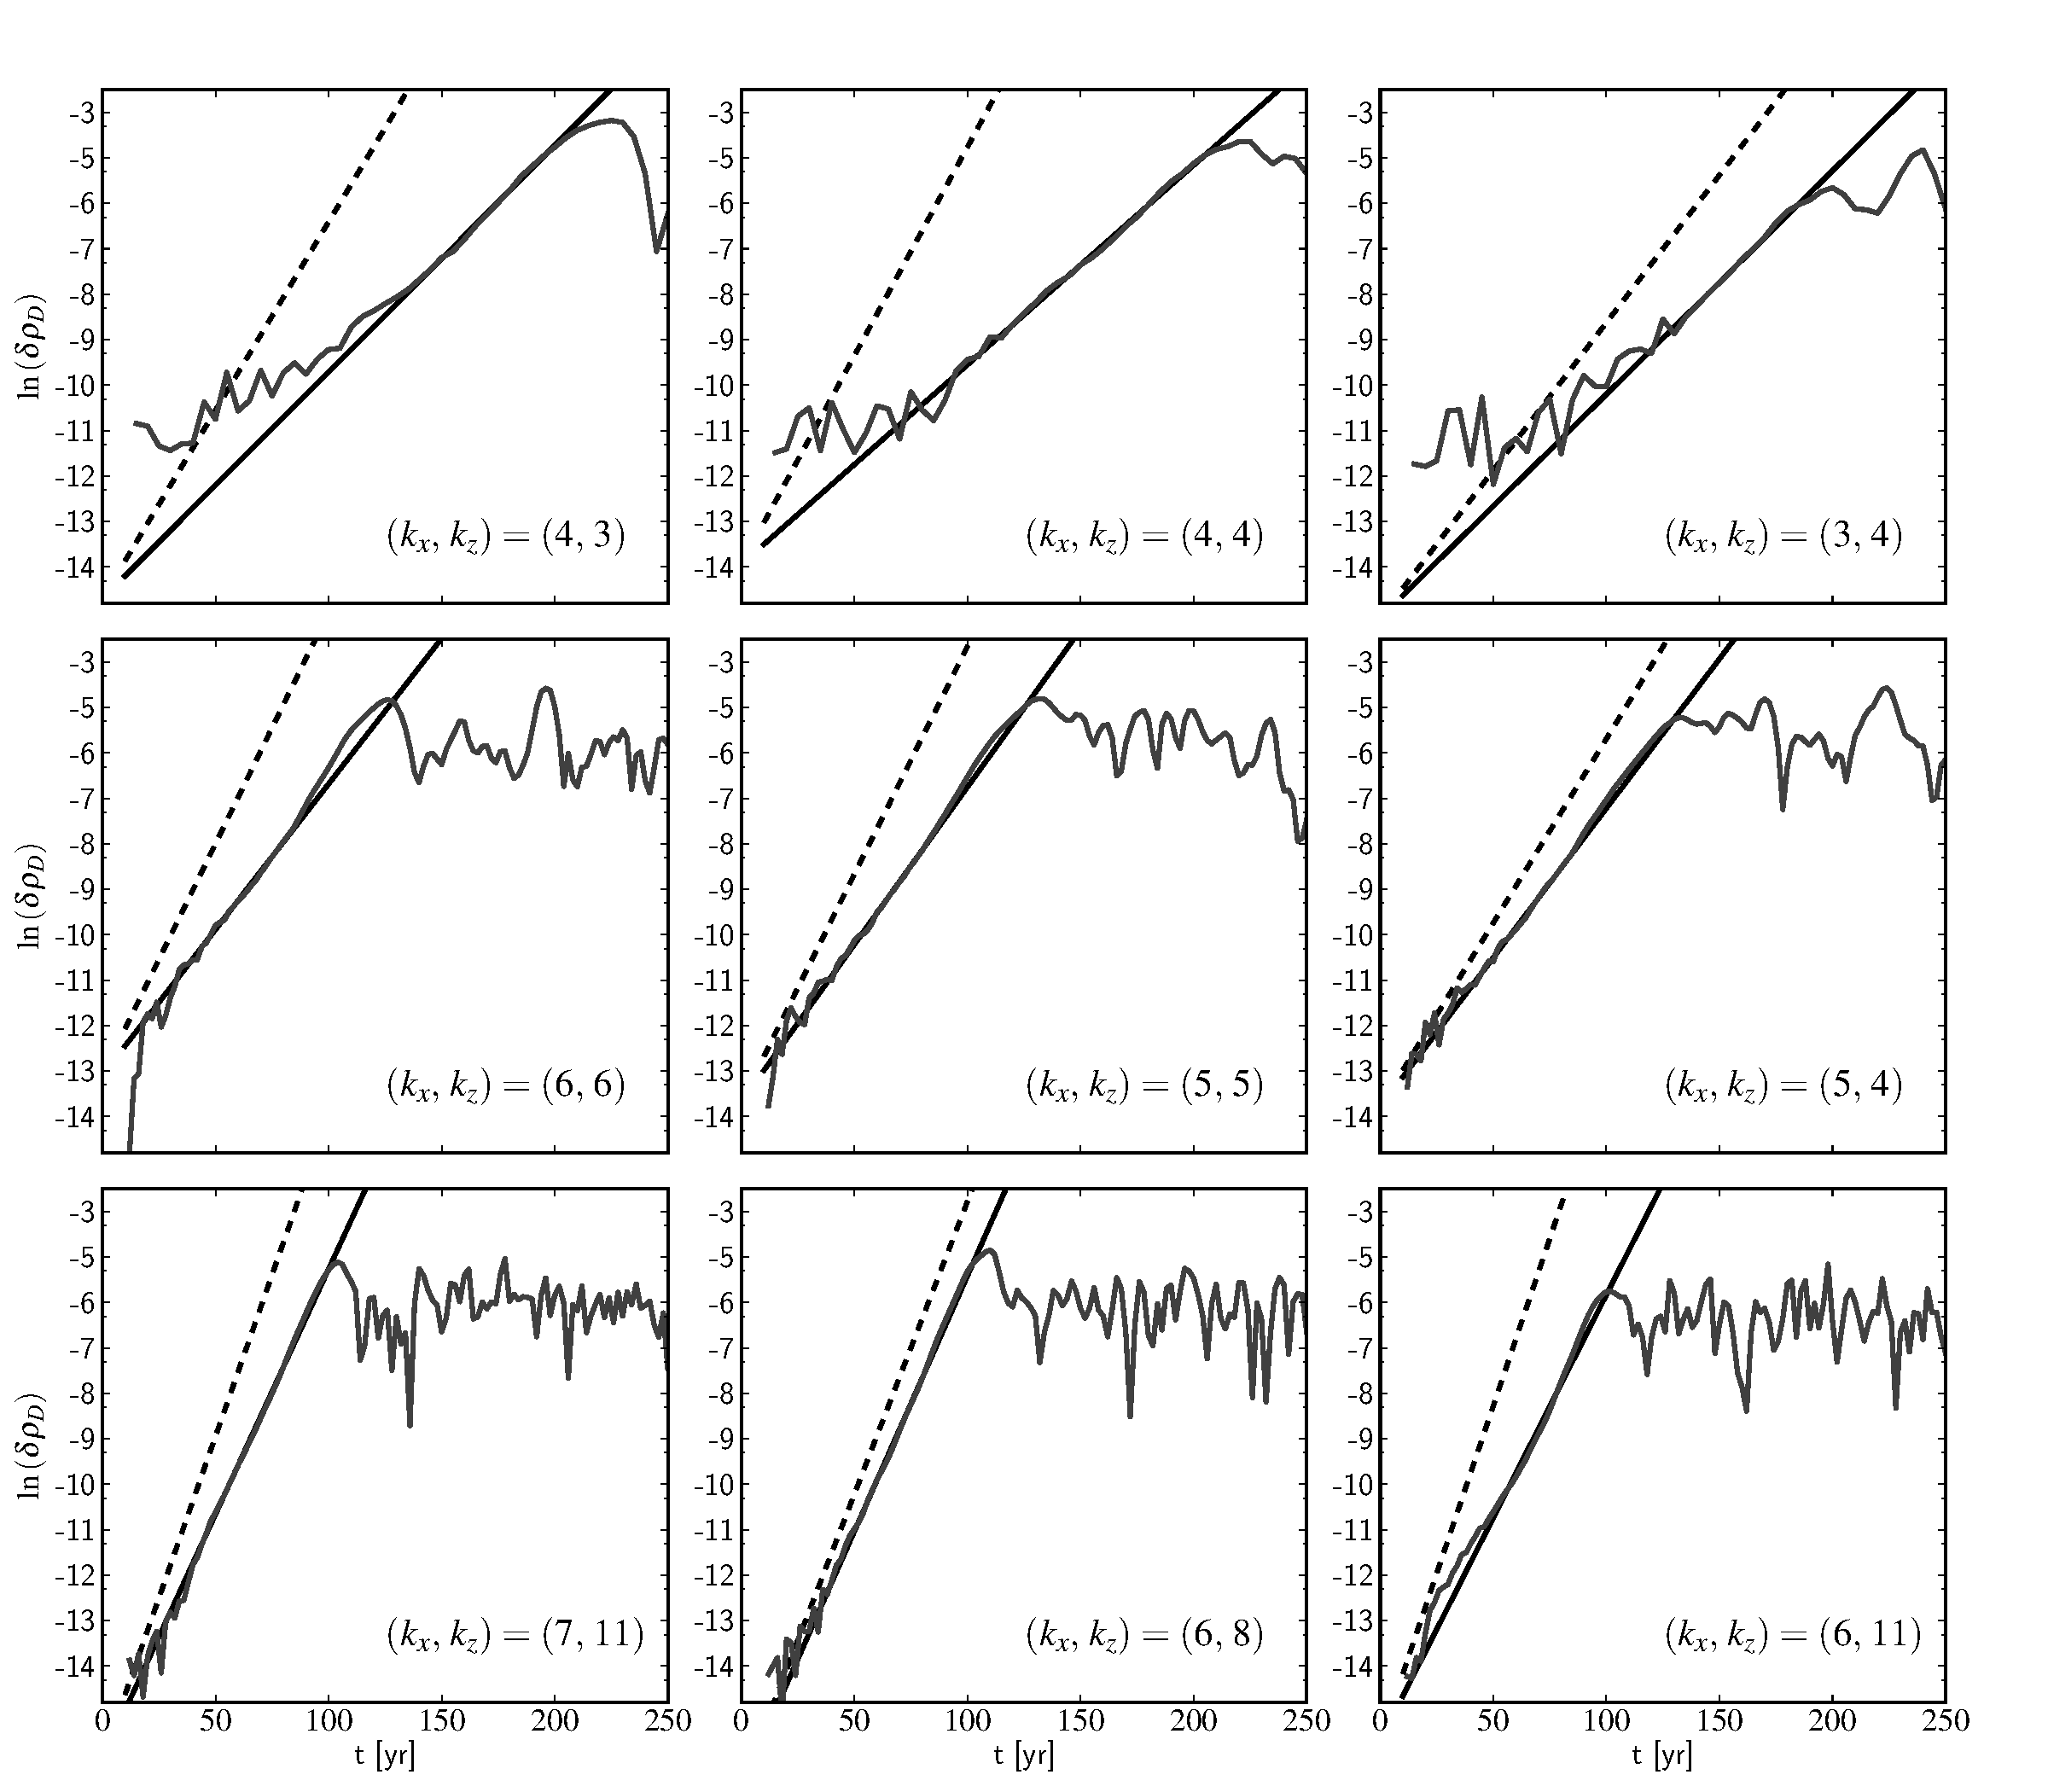
\includegraphics[width=0.98\linewidth]{figures/fig8}
   \caption{Czasowa ewolucja amplitud dominujących modów niestabilności
      strumieniowej mierzona dla zaburzenia gęstości (szara linia) wraz z
      dopasowaniem~\mref{eq:fit} (czarna linia) i~przewidywanym tempem wzrostu
      wynikającym z~liniowej analizy stabilności (linia przerywana).
      Rozwiązanie równania~\mref{eq:linset} jest określone na podstawie
      parametrów średnich kwadratowej łatki ulokowanej na $R=3\AU$ dla symulacji
BB3d (górny panel), BB (środkowy panel) and BBh (dolny panel).  } \label{fig8}
\end{figure}

\par Kolejnym argumentem potwierdzającym zgodność wyników z~liniową analizą
stabilności jest przedstawiony na Rysunku~\ref{fig9} wykres konturowy tempa
wzrostu wynikający z~rozwiązania równania~\mref{eq:disprel} w~zależności od
liczby falowej. Wyraźnie widać na nim, że najszybciej rosnące mody
niestabilności strumieniowej układają się w~charakterystyczny grzbiet w~kierunku
rosnących $k_x$ i~$k_z$.  Wykres tworzony jest dla stanu średniego w~łatce dla
czasu $T_{\textrm{ref}}$.  Następnie 9 dominujących modów wybranych wedle
kryterium opisywanego wcześniej jest zaznaczane przy użyciu punktów. Procedura
jest powtarzana dla symulacji o tych samych parametrach początkowych, ale
różnych rozdzielczościach.  Powyższy schemat działania pozwala potwierdzić, że
liczby falowe dominujących modów wzbudzanych w~eksperymencie numerycznym,
układają wzdłuż wspomnianego wcześniej grzbietu. Jedynym czynnikiem
ograniczającym wzrost modów krótkofalowych jest niewystarczająca rozdzielczość
domeny obliczeniowej. Dla serii symulacji BB3d, BB, BBh efektywna rozdzielczość
siatki wyniosła odpowiednio $150^2, 300^2, 600^2$ komórek obliczeniowych.
Dominujące mody symulacji o najniższej rozdzielczości grupują się poniżej
konturu ''$(-1.0)$'', zaś dla najwyższej praktycznie wszystkie mają tempo
wzrostu powyżej $0.1$. Podobne zachowanie jest widoczne dla pozostałych
symulacji dla których przeprowadzono testy zbieżności, tj. AB, ABh (prawy panel
na rysunku~\ref{fig9}). Przypuszczalnym powodem obecności wyraźnego obcięcia dla
krótki długości fali w~przeprowadzonych symulacjach jest wewnętrzną, numeryczna
dyfuzyjność metody RTVD użytej w~PIERNIKu. Z przeprowadzonych analiz wynika, że
używane algorytmy numeryczne potrzebują przynajmniej 32 komórek obliczeniowych
na długość fali niestabilnego modu, aby poprawnie oddać jego tempo wzrostu.
Należy przy tym zauważyć, że krótsze mody zawierające się w~mniejszej liczbie
komórek nadal pozostają niestabilne, aczkolwiek mogą wykazywać mniejsze tempo
wzrostu niż to wynikające z~liniowej analizy stabilności.
%
\begin{figure*}
  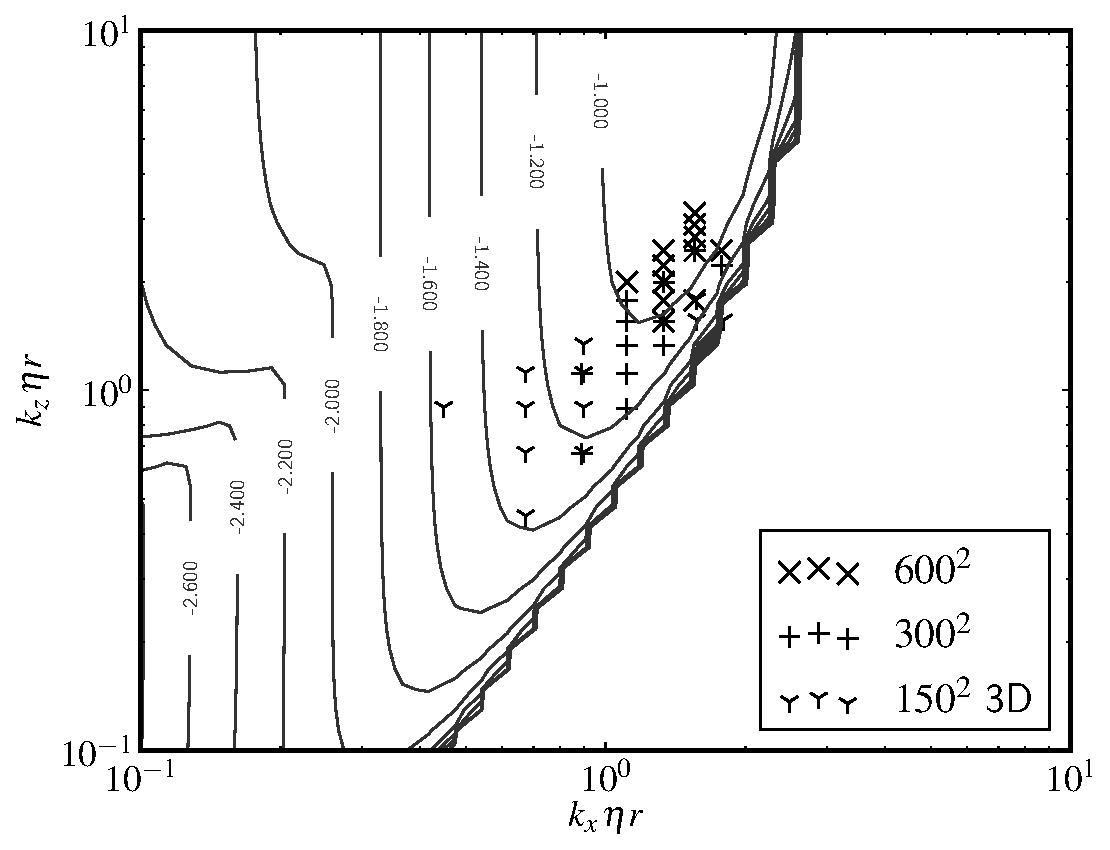
\includegraphics[width=0.48\linewidth]{figures/fig9a}
  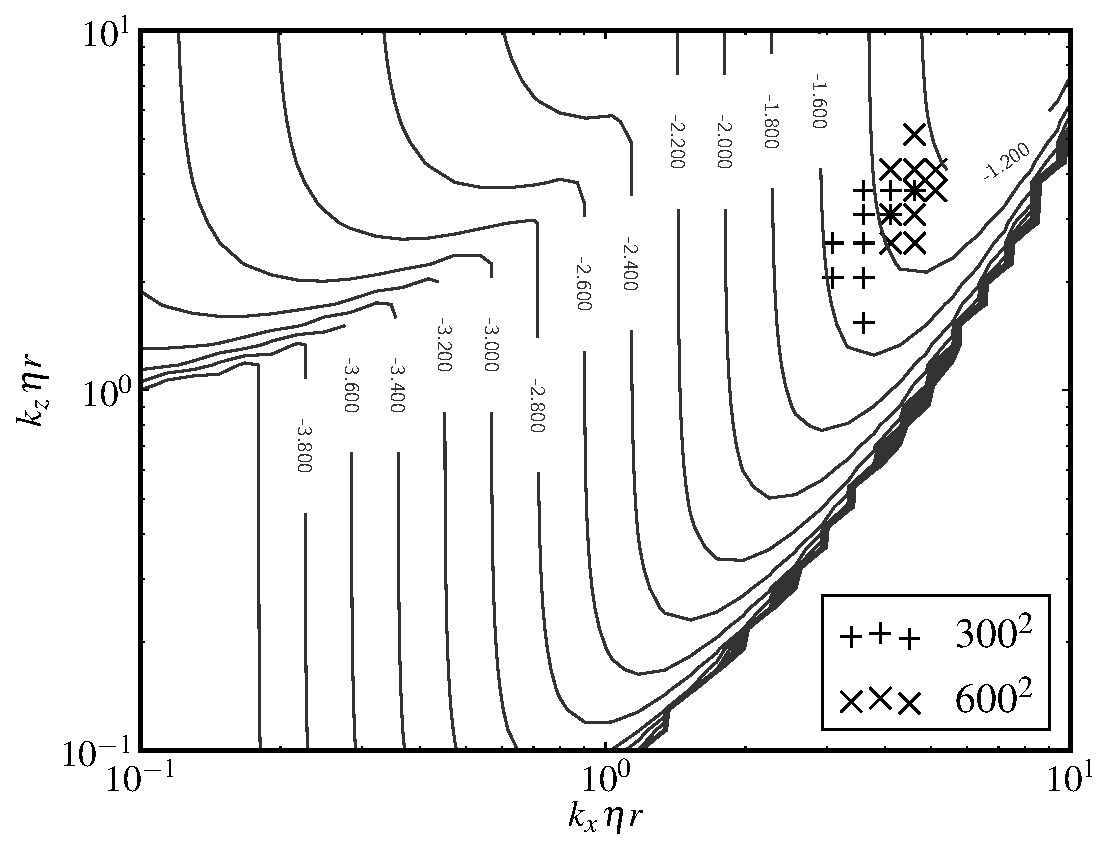
\includegraphics[width=0.48\linewidth]{figures/fig9b}
  \caption{Dziewięć najszybciej rosnących modów o liczbach falowych $(k_x, k_z)$
     wyodrębnionych z~symulacji o tych samych fizycznych warunkach początkowych,
     lecz różnej rozdzielczości siatki obliczeniowej. (lewy panel: BB3d, BB,
     BBh, prawy: AB, ABh). Kontury wyznaczają tempo wzrostu $\log_{10}( s_0(k_x,
  k_z))$ wynikające z~rozwiązania równania~ \mref{eq:disprel} dla średniego
  stanu wybranych łatek w~momencie czasu  $T = T_{\textrm{ref}}$ (dla porównania
  por. Rysunek.~2 z~pracy~\cite{YG05})}
   \label{fig9}
\end{figure*}
%
\par Jako że niestabilność strumieniowa w~ogólności ,,preferuje'' krótsze
długości fali, zwiększenia rozdzielczości zawsze prowadzi do wytworzenia
to zagęszczeń o coraz mniejszych rozmiarach w~krótszym czasie~(por.
Rysunek~\ref{fig10}).  Jednakże przeprowadzone symulacje odtwarzają w~dobrym
stopniu przewidywania liniowej analizy stabilności, a także są w~stanie oddać
wszystkie efekty jakościowe, np. ,,kawitację'' (por. Rysunek~\ref{fig3}) czy
gwałtowne rozmycie niestabilności w~przypadku $\epsilon=0.2$ i~$a=10\cm$, bez
względu na rozmiar najmniejszej komórki obliczeniowej.

\begin{figure}
   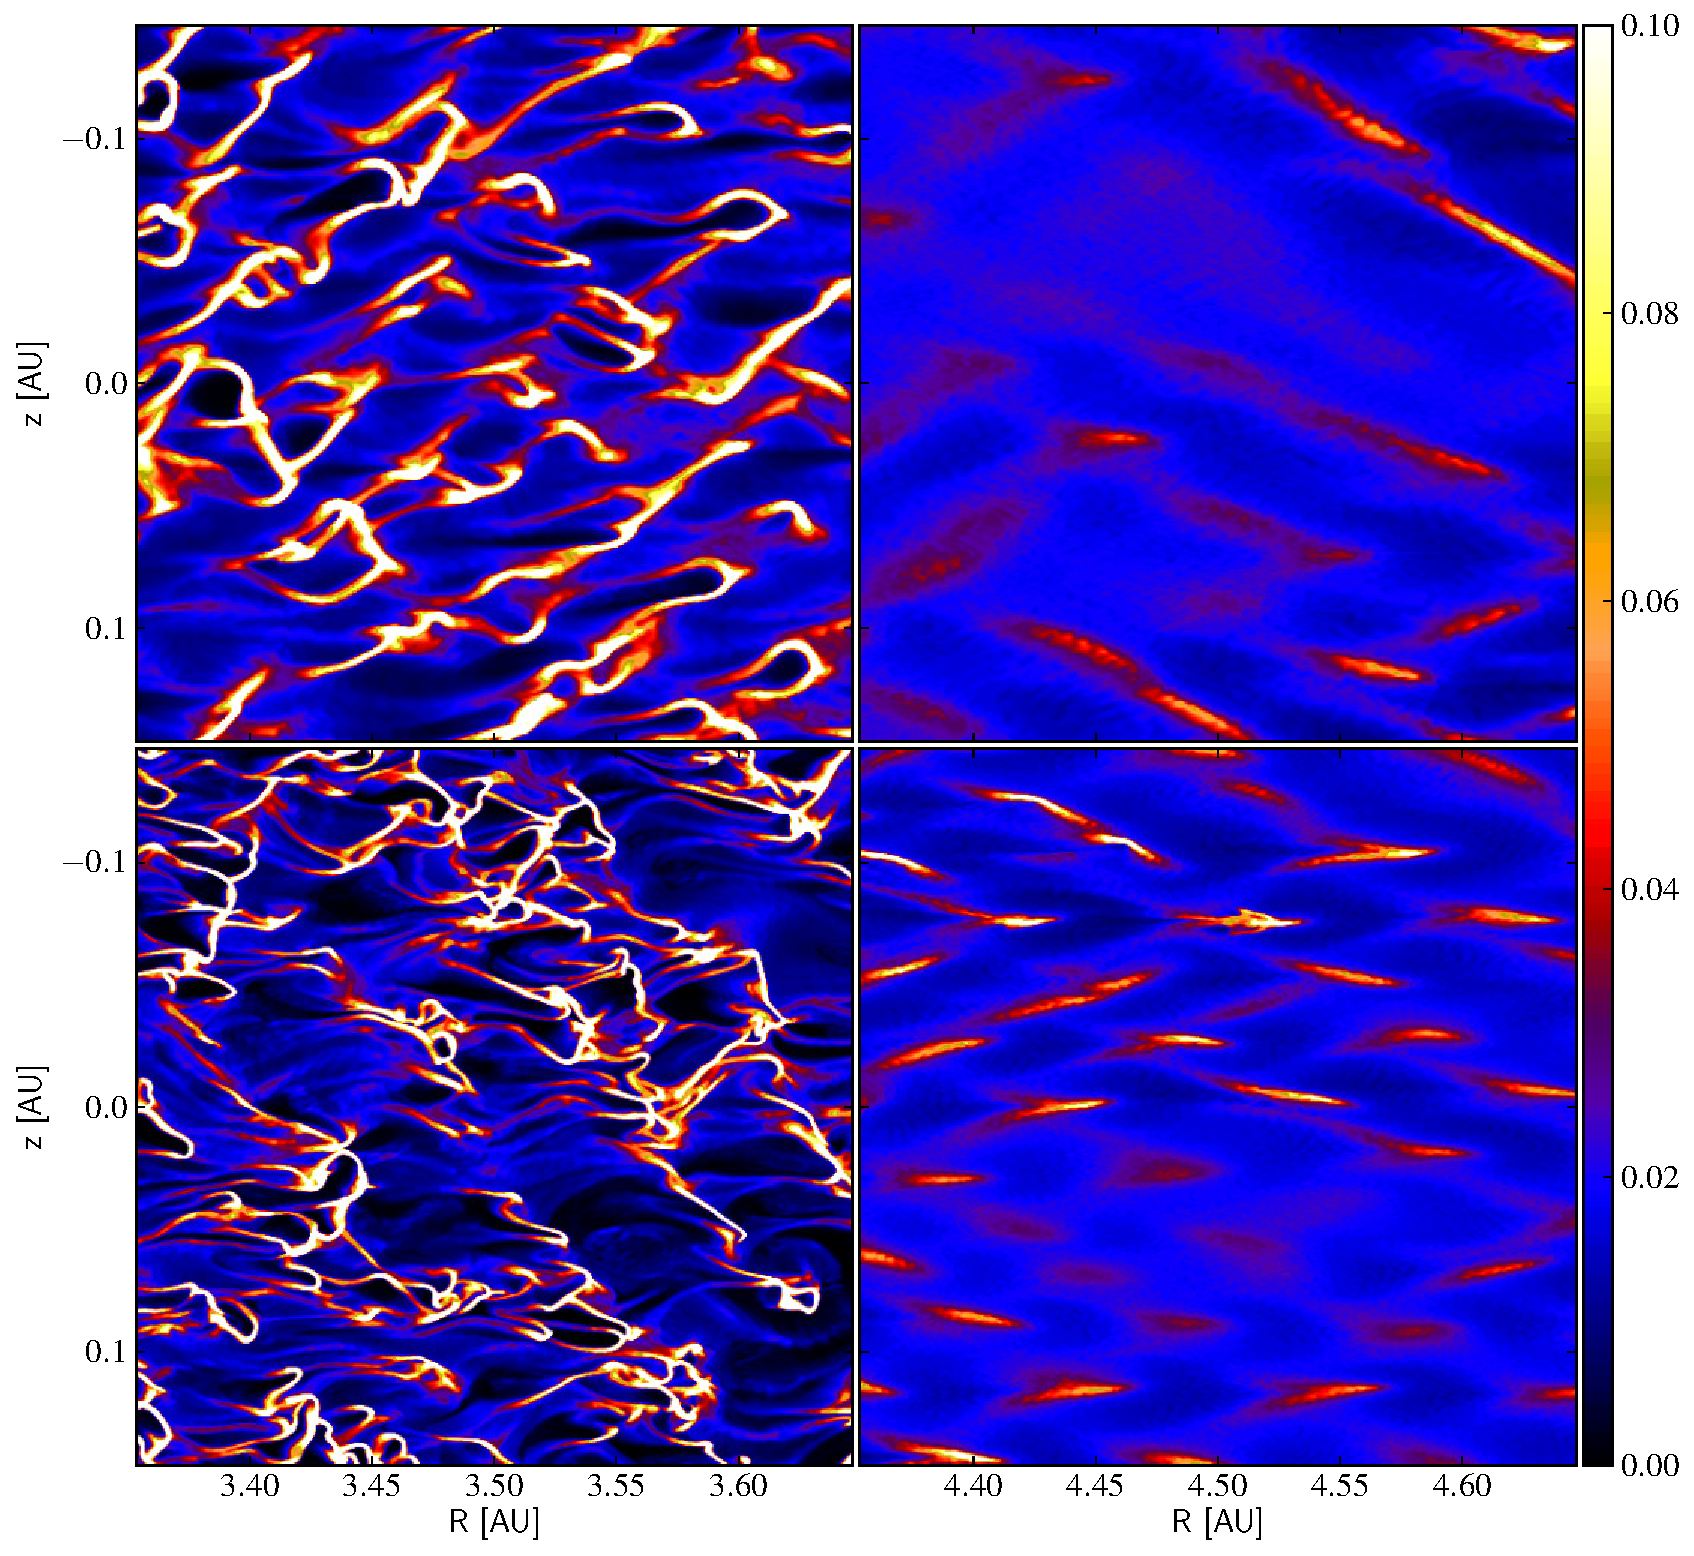
\includegraphics[width=0.98\linewidth]{figures/fig10}
   \caption{Migawki gęstości pyłu dla $t = 160\yr$ dla łatek pochodzących z
      orbit $R=3.5$ i~$4.5\AU$ wyodrębnione z~symulacji o tych samych warunkach
      początkowych lecz różnej rozdzielczości siatki obliczeniowej. Górny panel
      symulacja BB, zaś dolny symulacja BBh. Ze względu na właściwości
      dyfuzji numerycznej, wyższa rozdzielczość promuje krótsze długości
      fali}
   \label{fig10} 
\end{figure}

\section{Symulacje trójwymiarowe z udziałem samograwitacji}
Przedmiotem dotychczasowych badań była niestabilność strumieniowa bez udziału
samograwitacji. Pokazaliśmy, że w dwuwymiarowym przybliżeniu tempo wzrostu
niestabilności w liniowym zakresie bardzo dobrze zgadza się z przewidywaniami
liniowej teorii, a zagęszczenia pyłu powstające w nieliniowej fazie rozwoju
niestabilności osiągają amplitudę przewyższającą gęstość początkową od jednego
do dwóch rzędów wielkości. W modelu 3d tempo wzrostu jest wyraźnie pomniejszone
względem przewidywań liniowej teorii z powodu mniejszej dostępnej rozdzielczości
siatki obliczeniowej, ale fluktuacje gęstości oscylują na podobnym poziomie jak
w symulacjach dwuwymiarowych. Wynik ten stanowi silną przesłankę, że warunki dla
niestabilności grawitacyjnej są w niewielkim stopniu zależne od rozdzielczości
siatki. W~niniejszy rozdziale przedstawione zostały 2 symulacje pełnego,
trójwymiarowego modelu dysku: z~uwzględnieniem efektów samograwitacji płynów
(BD3dS) oraz bez jej udziału (BB3d, BD3d). Symulacja BB3d została przeprowadzana
jako trójwymiarowy analog wcześniej opisywanych symulacji dwuwymiarowych.


\begin{table}
   \centering
   \begin{tabular}{cccccc}
      \hline
      Nazwa & $N_r \times N_\varphi \times N_z$ &
      $a$~[cm] & $\epsilon$ & $T_\textrm{end}$~[yr] \\
      \hline
      BD3d  &  $2560  \times 512 \times 192$  & 50  & 3.0 & 500  \\
      BD3dS &  $2560  \times 512 \times 192$  & 50  & 3.0 & 300  \\
      BB3d  &  $2560  \times 512 \times 192$  & 50  & 1.0 & 500  \\
      \hline
   \end{tabular}
\caption{Parametry użyte w~symulacjach 3D. Kolumny opisują w~kolejności: oznaczenie
   kodowe symulacji, ilość komórek obliczeniowych w~kierunkach $r$, $\varphi$ i
   $z$, promień cząstek, początkowy stosunek gęstości pyłu do gęstości gazu,
całkowity czas trwania symulacji w~latach.}
\label{tab2}
\end{table}

%%%%%%%%%%%%%%%%%%%%%%%%%%%%%%%%%%%%%%%%%%%%%%%%%%%%%%%%%%%%%%%%%%%%%%%%%%%%%%%%
% vim: tw=80 ts=3: 

Wybrane migawki z trójwymiarowej ewolucji dysku w symulacji BD3d zostały
pokazane na rysunku~\ref{fig:slicenosg} dla czasów $t = 50, 100, 150, 200,
400$~lat. Przedstawione na tym rysunku rozkłady gęstości pyłu w cięciach
\textit{r-z} ujawniają duże podobieństwo wizualne do rozkładów gęstości w
symulacjach dwuwymiarowych. 
%
\begin{figure}
   \centering
   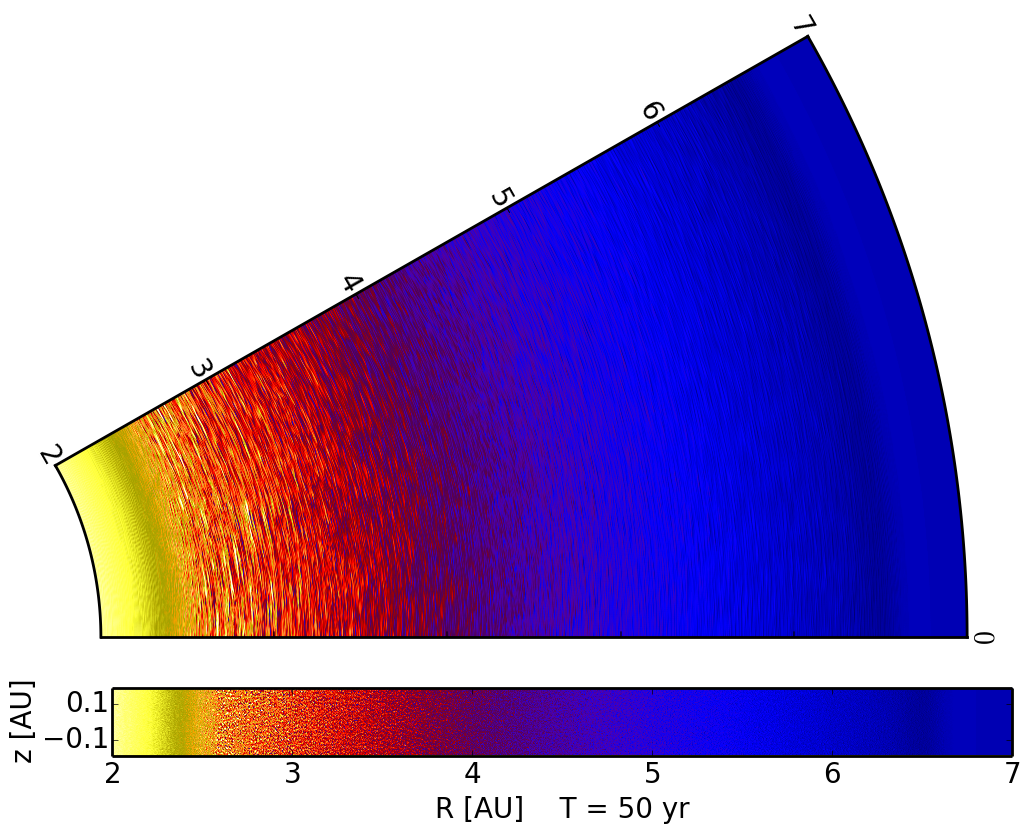
\includegraphics[width=0.44\linewidth]{figures/slice_nosg_01}
   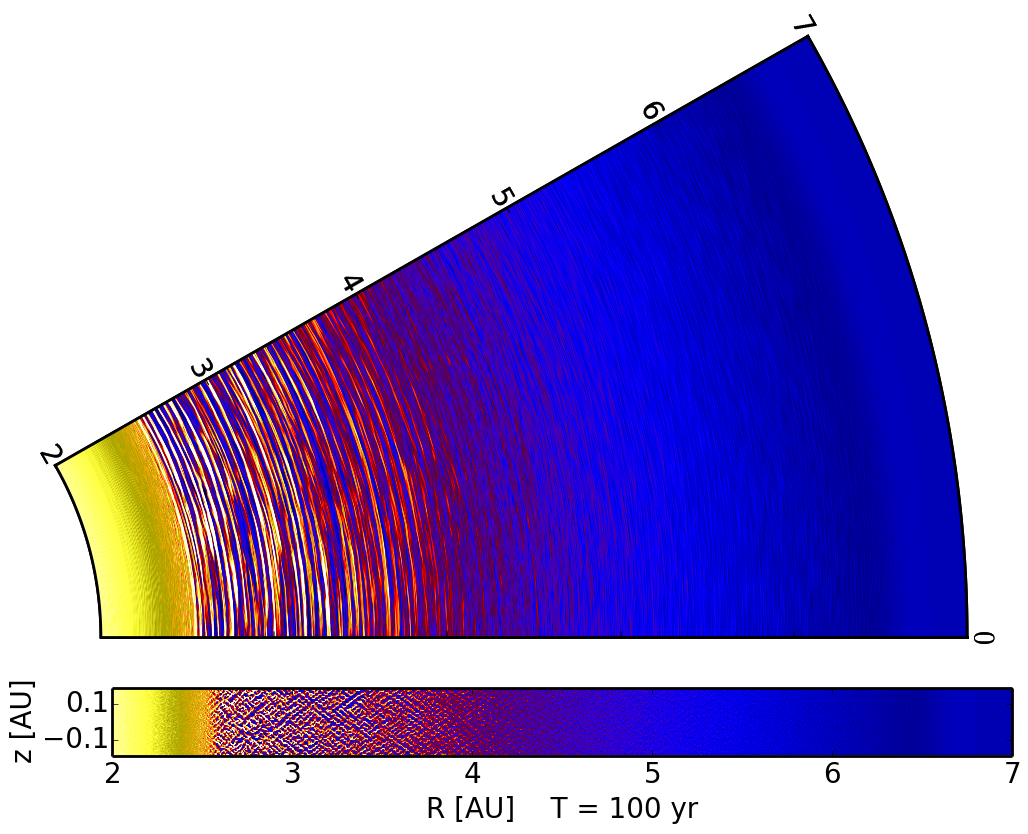
\includegraphics[width=0.44\linewidth]{figures/slice_nosg_02} \\
   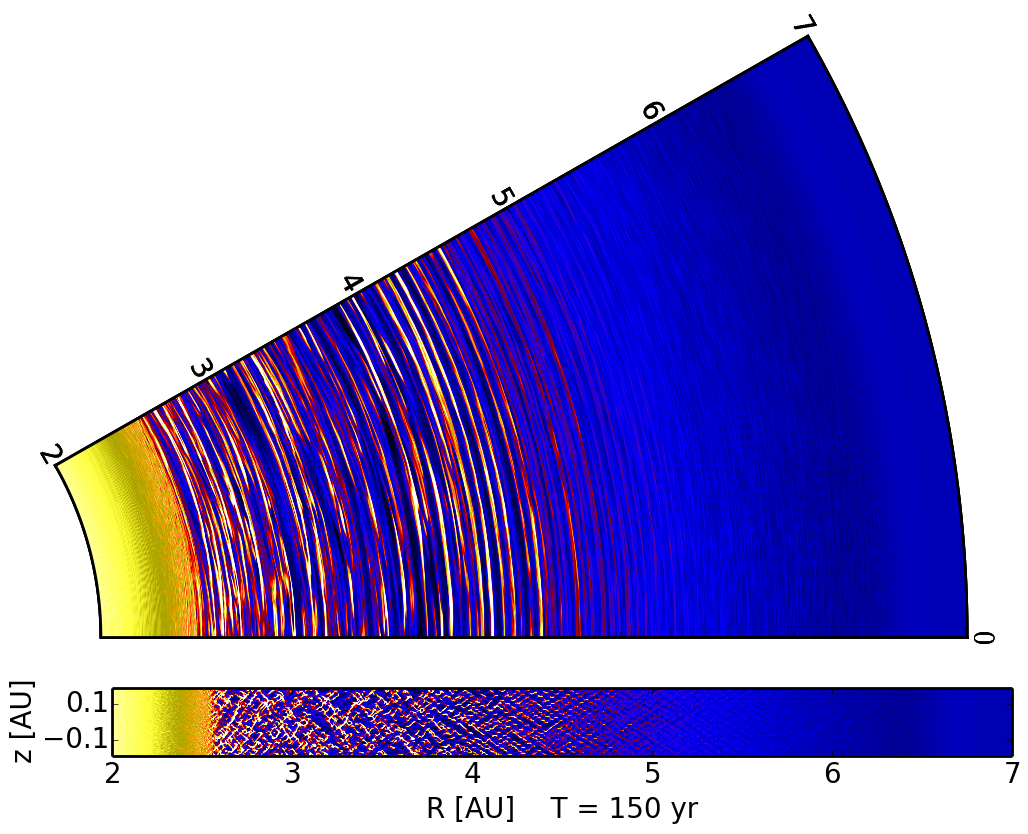
\includegraphics[width=0.44\linewidth]{figures/slice_nosg_03}
   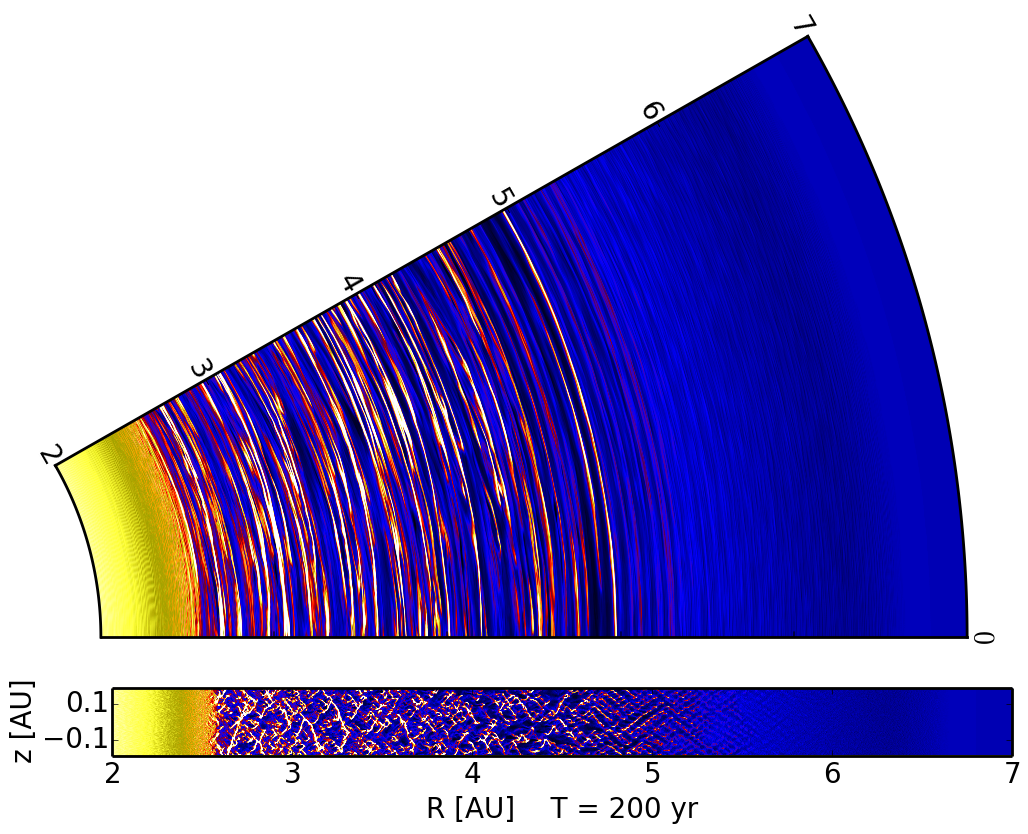
\includegraphics[width=0.44\linewidth]{figures/slice_nosg_04} \\
   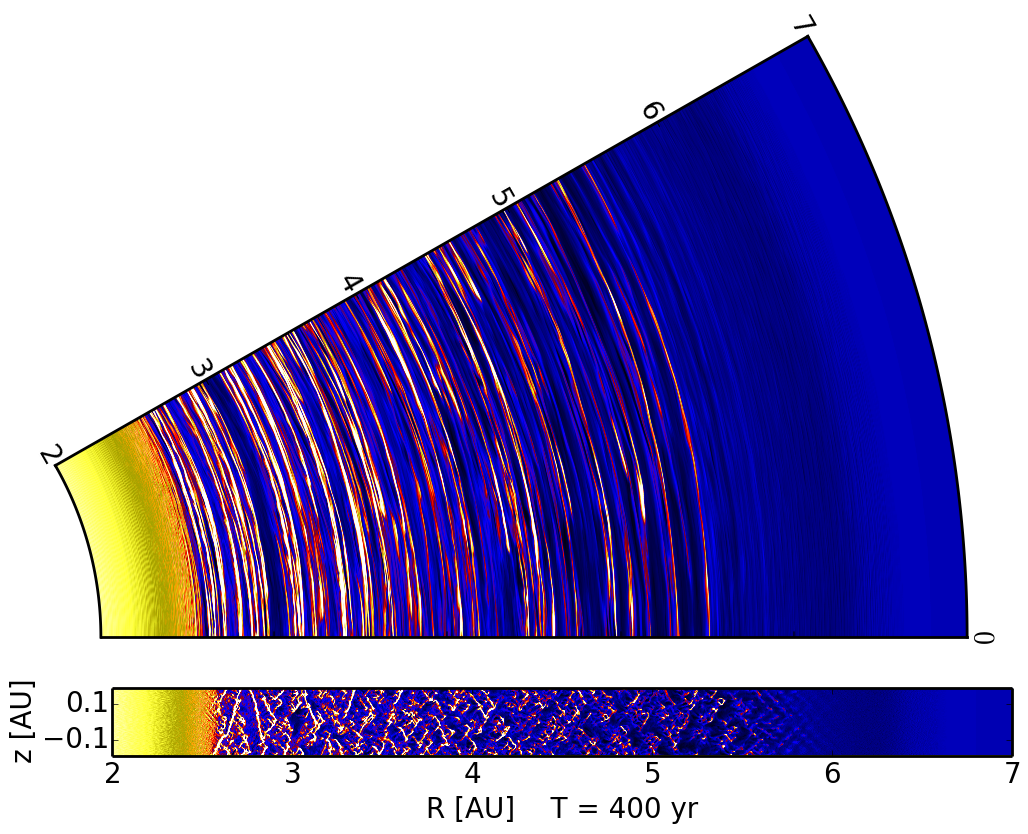
\includegraphics[width=0.44\linewidth]{figures/slice_nosg_05}
   \caption{
      Migawki z~symulacji BD3d obrazujące gęstość pyłu w~cięciach w
      płaszczyznach $R -\varphi$ oraz $R - z$ przechodzących przez środek 
   domeny obliczeniowej, dla czasów $t= 50, 100, 150, 200, 400$ lat}
   \label{fig:slicenosg}
\end{figure}
%
Początkowo w~rozkładzie gęstości pyłu wyłania się przedstawiony już wcześniej
ukośny wzór, będący superpozycją działania najbardziej niestabilnych modów.
Model trójwymiarowy pokazuje, że zagęszczenia widoczne w płaszczyźnie
\textit{r-z} są w rzeczywistości cięciami włókien rozciągłych w kierunku
azymutalnym. Liniowy zakres ewolucji niestabilności strumieniowej w 3D przebiega
zgodnie z przewidywaniami liniowej analizy stabilności przedstawionej dla
przypomnienia w rozdziale drugim. Najszybciej rosnące mody niestabilności
strumieniowej lokują się na mapach stabilności (Rys.~\ref{fig9} dla symulacji
BB3d oraz Rys.~\ref{fig:map3d} dla symulacji BD3d) wzdłuż grzbietu
wyznaczającego największe analityczne tempa wzrostu wynikające z liniowej
analizy stabilności. Wybrane migawki z trójwymiarowej
ewolucji dysku w symulacji BD3d zostały pokazane na rysunku~\ref{fig:slicenosg}
dla czasów $t =  50, 100, 150, 200, 400$ lat. Przedstawione na tym rysunku
cięcia zarówno w płaszczyźnie \textit{r-z} jak i \textit{r-}$\varphi$ pokazują, że
gęstość pyłu mierzona wzdłuż włókien wykazuje modulację wskazującą na
potrzebę uwzględnienia azymutalnej liczby falowej w liniowej analizie
niestabilności strumieniowej. Jednakże, tempo wzrostu mierzone w liniowym
zakresie pozostaje zgodne z przewidywaniami teorii dla przybliżenia
dwuwymiarowego. Odstępstwa od osiowej symetrii są widoczne, lecz praktycznie nie
wpływają na zachowanie się niestabilności w liniowym zakresie (por.
Rysunek~\ref{fig:slicenosg}. Podobnie jak w~analogicznych symulacjach 2D,
saturacja niestabilności następuje po lokalnym wzroście gęstości pyłu o
$1\div1.5$ rzędu wielkości
%
\begin{figure}[h]
   \centering
   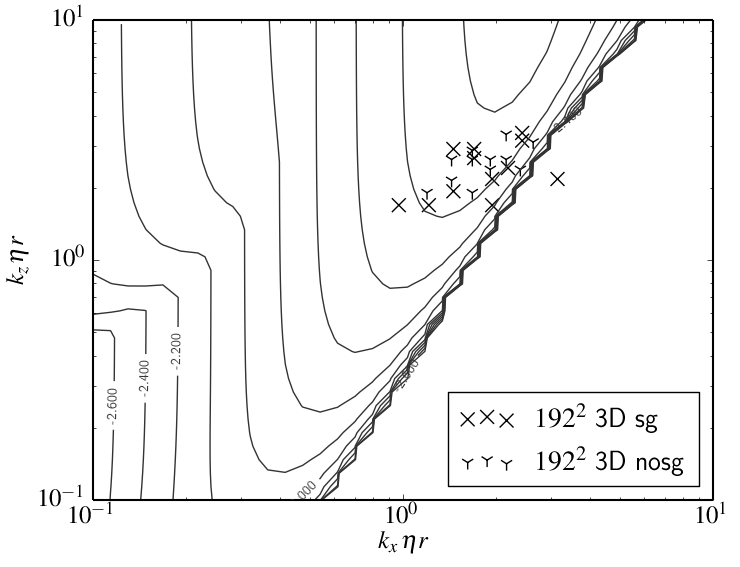
\includegraphics[width=0.5\linewidth]{figures/3d_map_x3_50.png}
   \caption{
      Dziewięć najszybciej rosnących modów o liczbach falowych (kx; kz)
      wyodrębnionych z symulacji o tych samych fizycznych warunkach
      początkowych, różniących się uwzględnieniem bądź nieuwzględnieniem
      samograwitacji (BD3d, BD3dS).  Kontury wyznaczają tempo wzrostu
      $\log_{10}(s_0(k_x, k_z))$ wynikające z~rozwiązania równania~
      \mref{eq:disprel} dla średniego stanu wybranych łatek w~momencie
      czasu $T = 80$~lat}
   \label{fig:map3d}
\end{figure}
% x3_50n.png
\par Obraz niestabilności strumieniowej diametralnie się zmienia po
uwzględnieniu samograwitacji pyłu. Początkowo ewolucja przebiega wzdłuż tego
samego scenariusza, dominujące mody niestabilności strumieniowej formują
charakterystyczny wzór--kratkę (Rysunek~\ref{fig:slicesg}). Tempo tworzenia się
zagęszczeń w~tej fazie $(50 - 100\yr)$ jest takie samo jak w~przypadku bez
samograwitacji~(Rysunek~\ref{fig:modes3d}). Ponadto dominujące mody lokują się
na mapie stabilności w~obszarze o największym tempie wzrostu wynikających z
liniowej analizy (Rysunek~\ref{fig:map3d}).
%
\begin{figure}
   \centering
   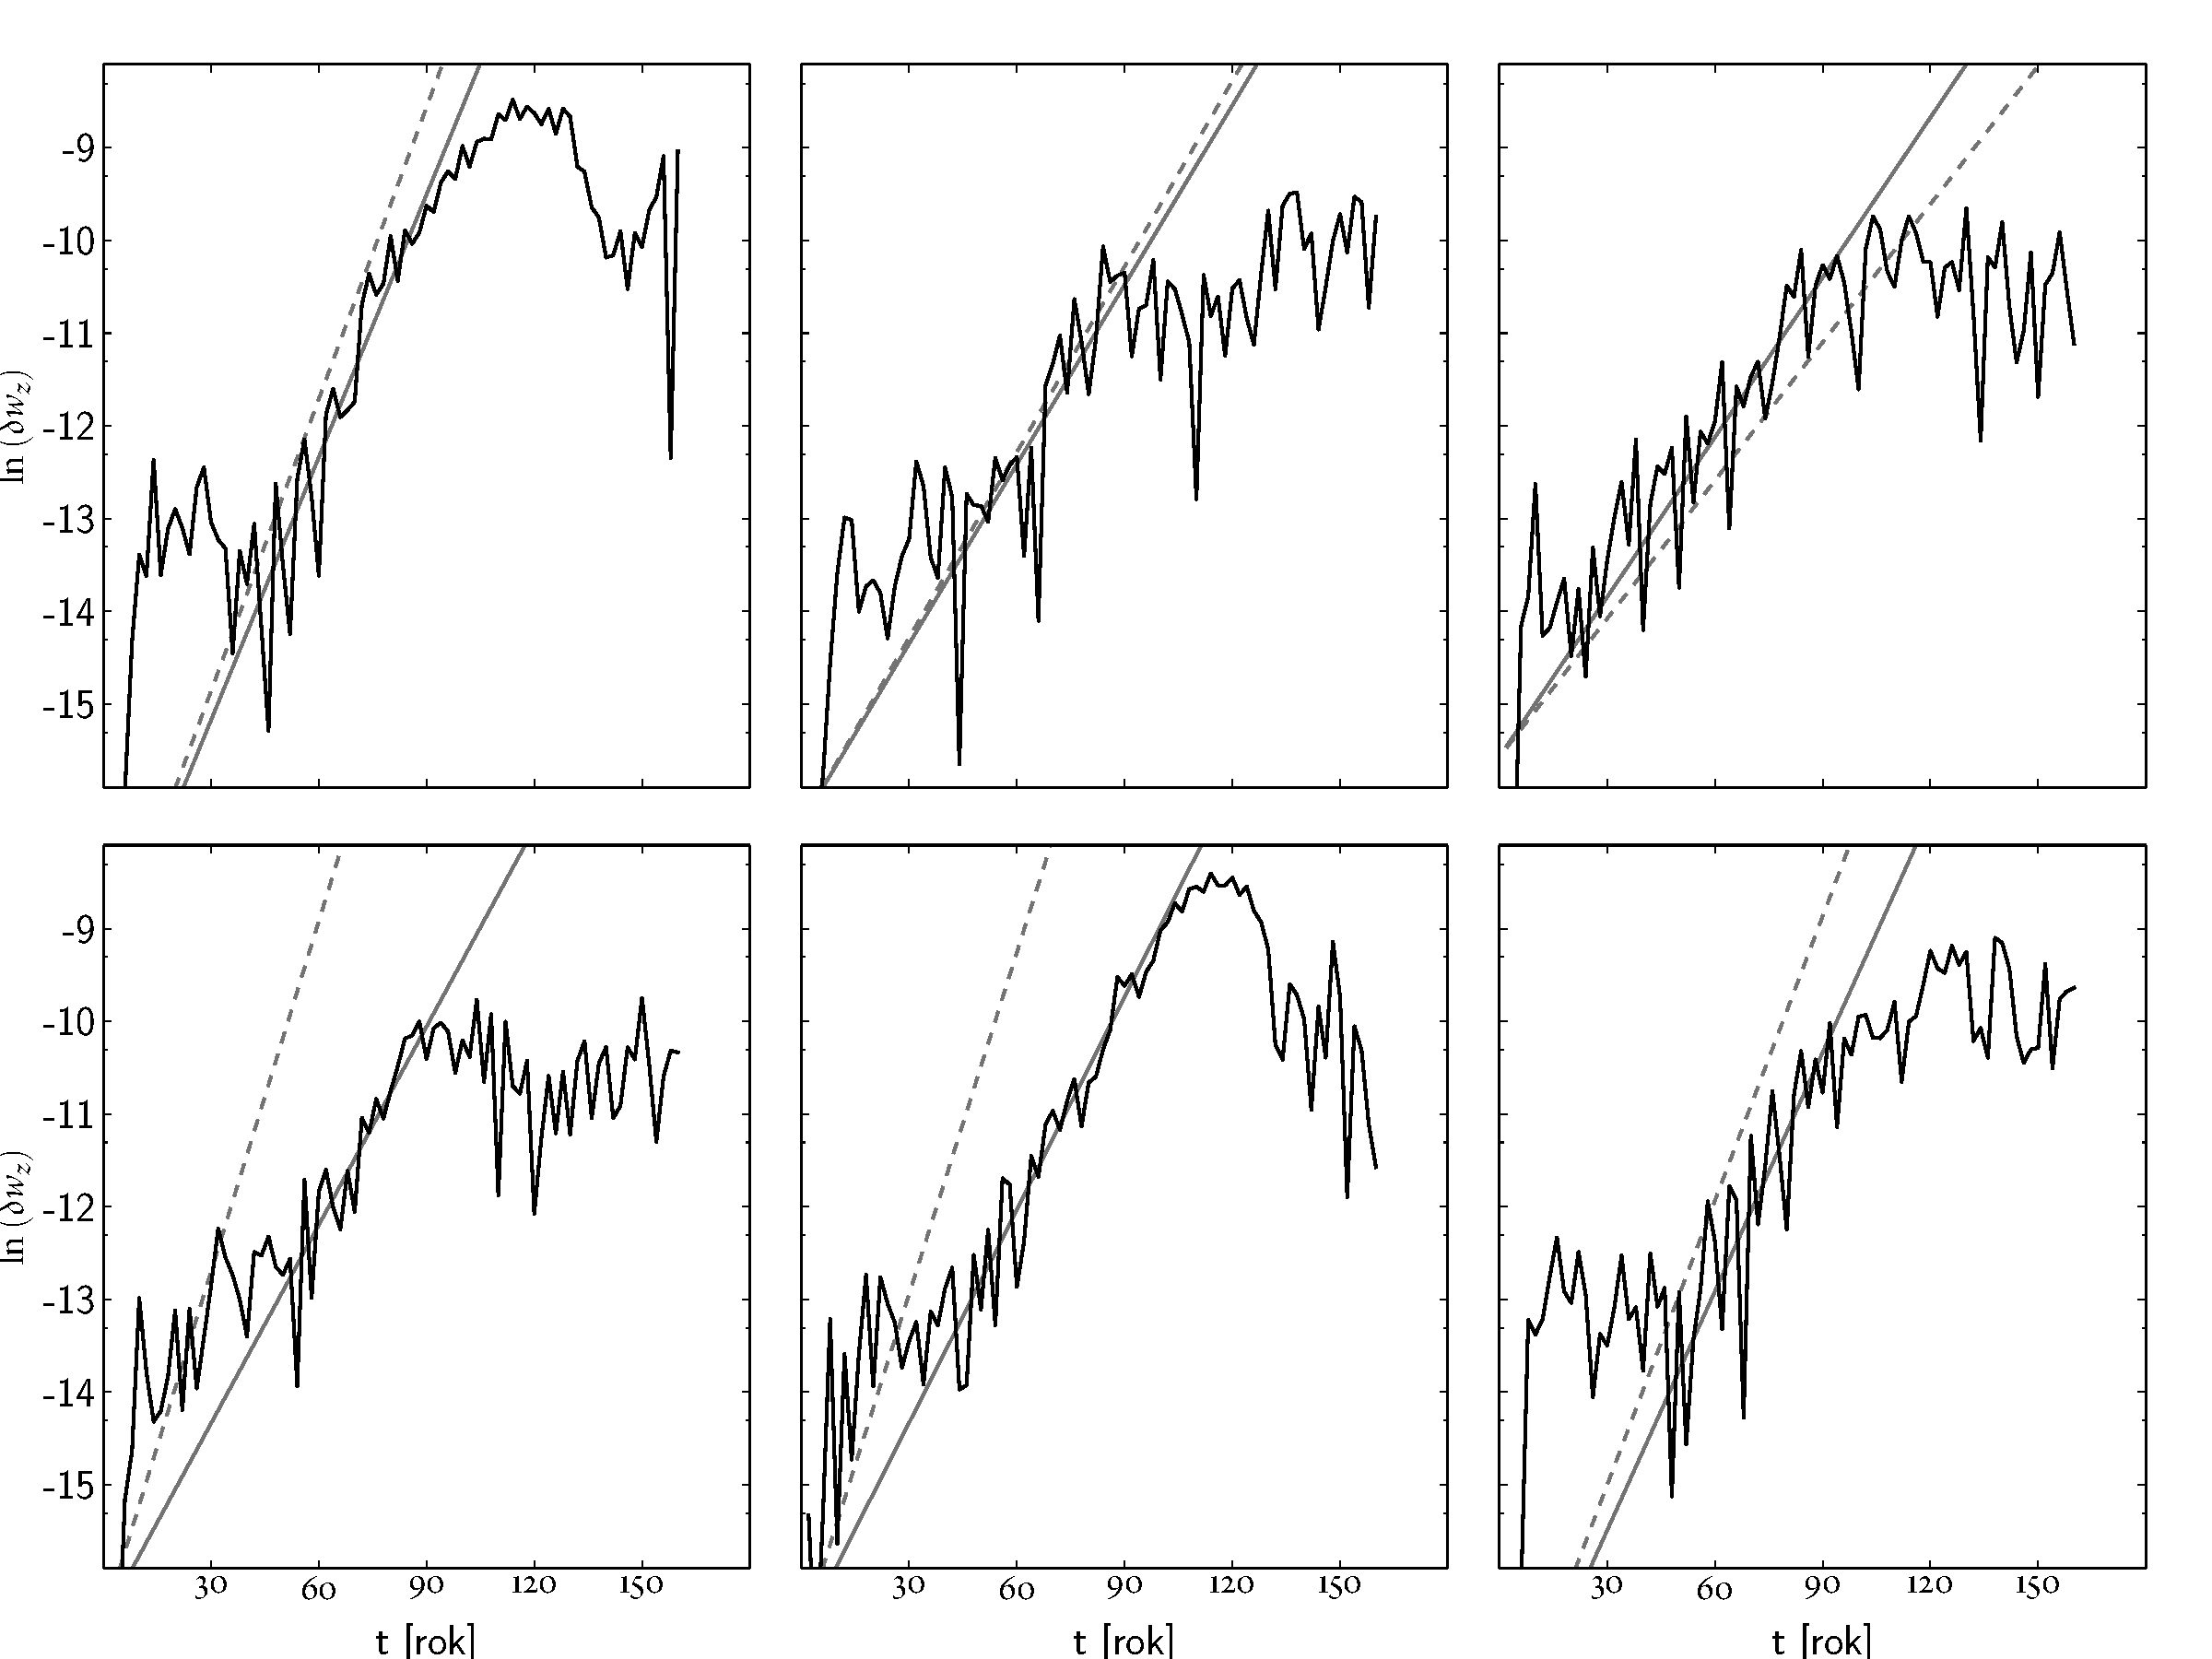
\includegraphics[height=0.44\textheight]{figures/nosg_vlzd_growth}
   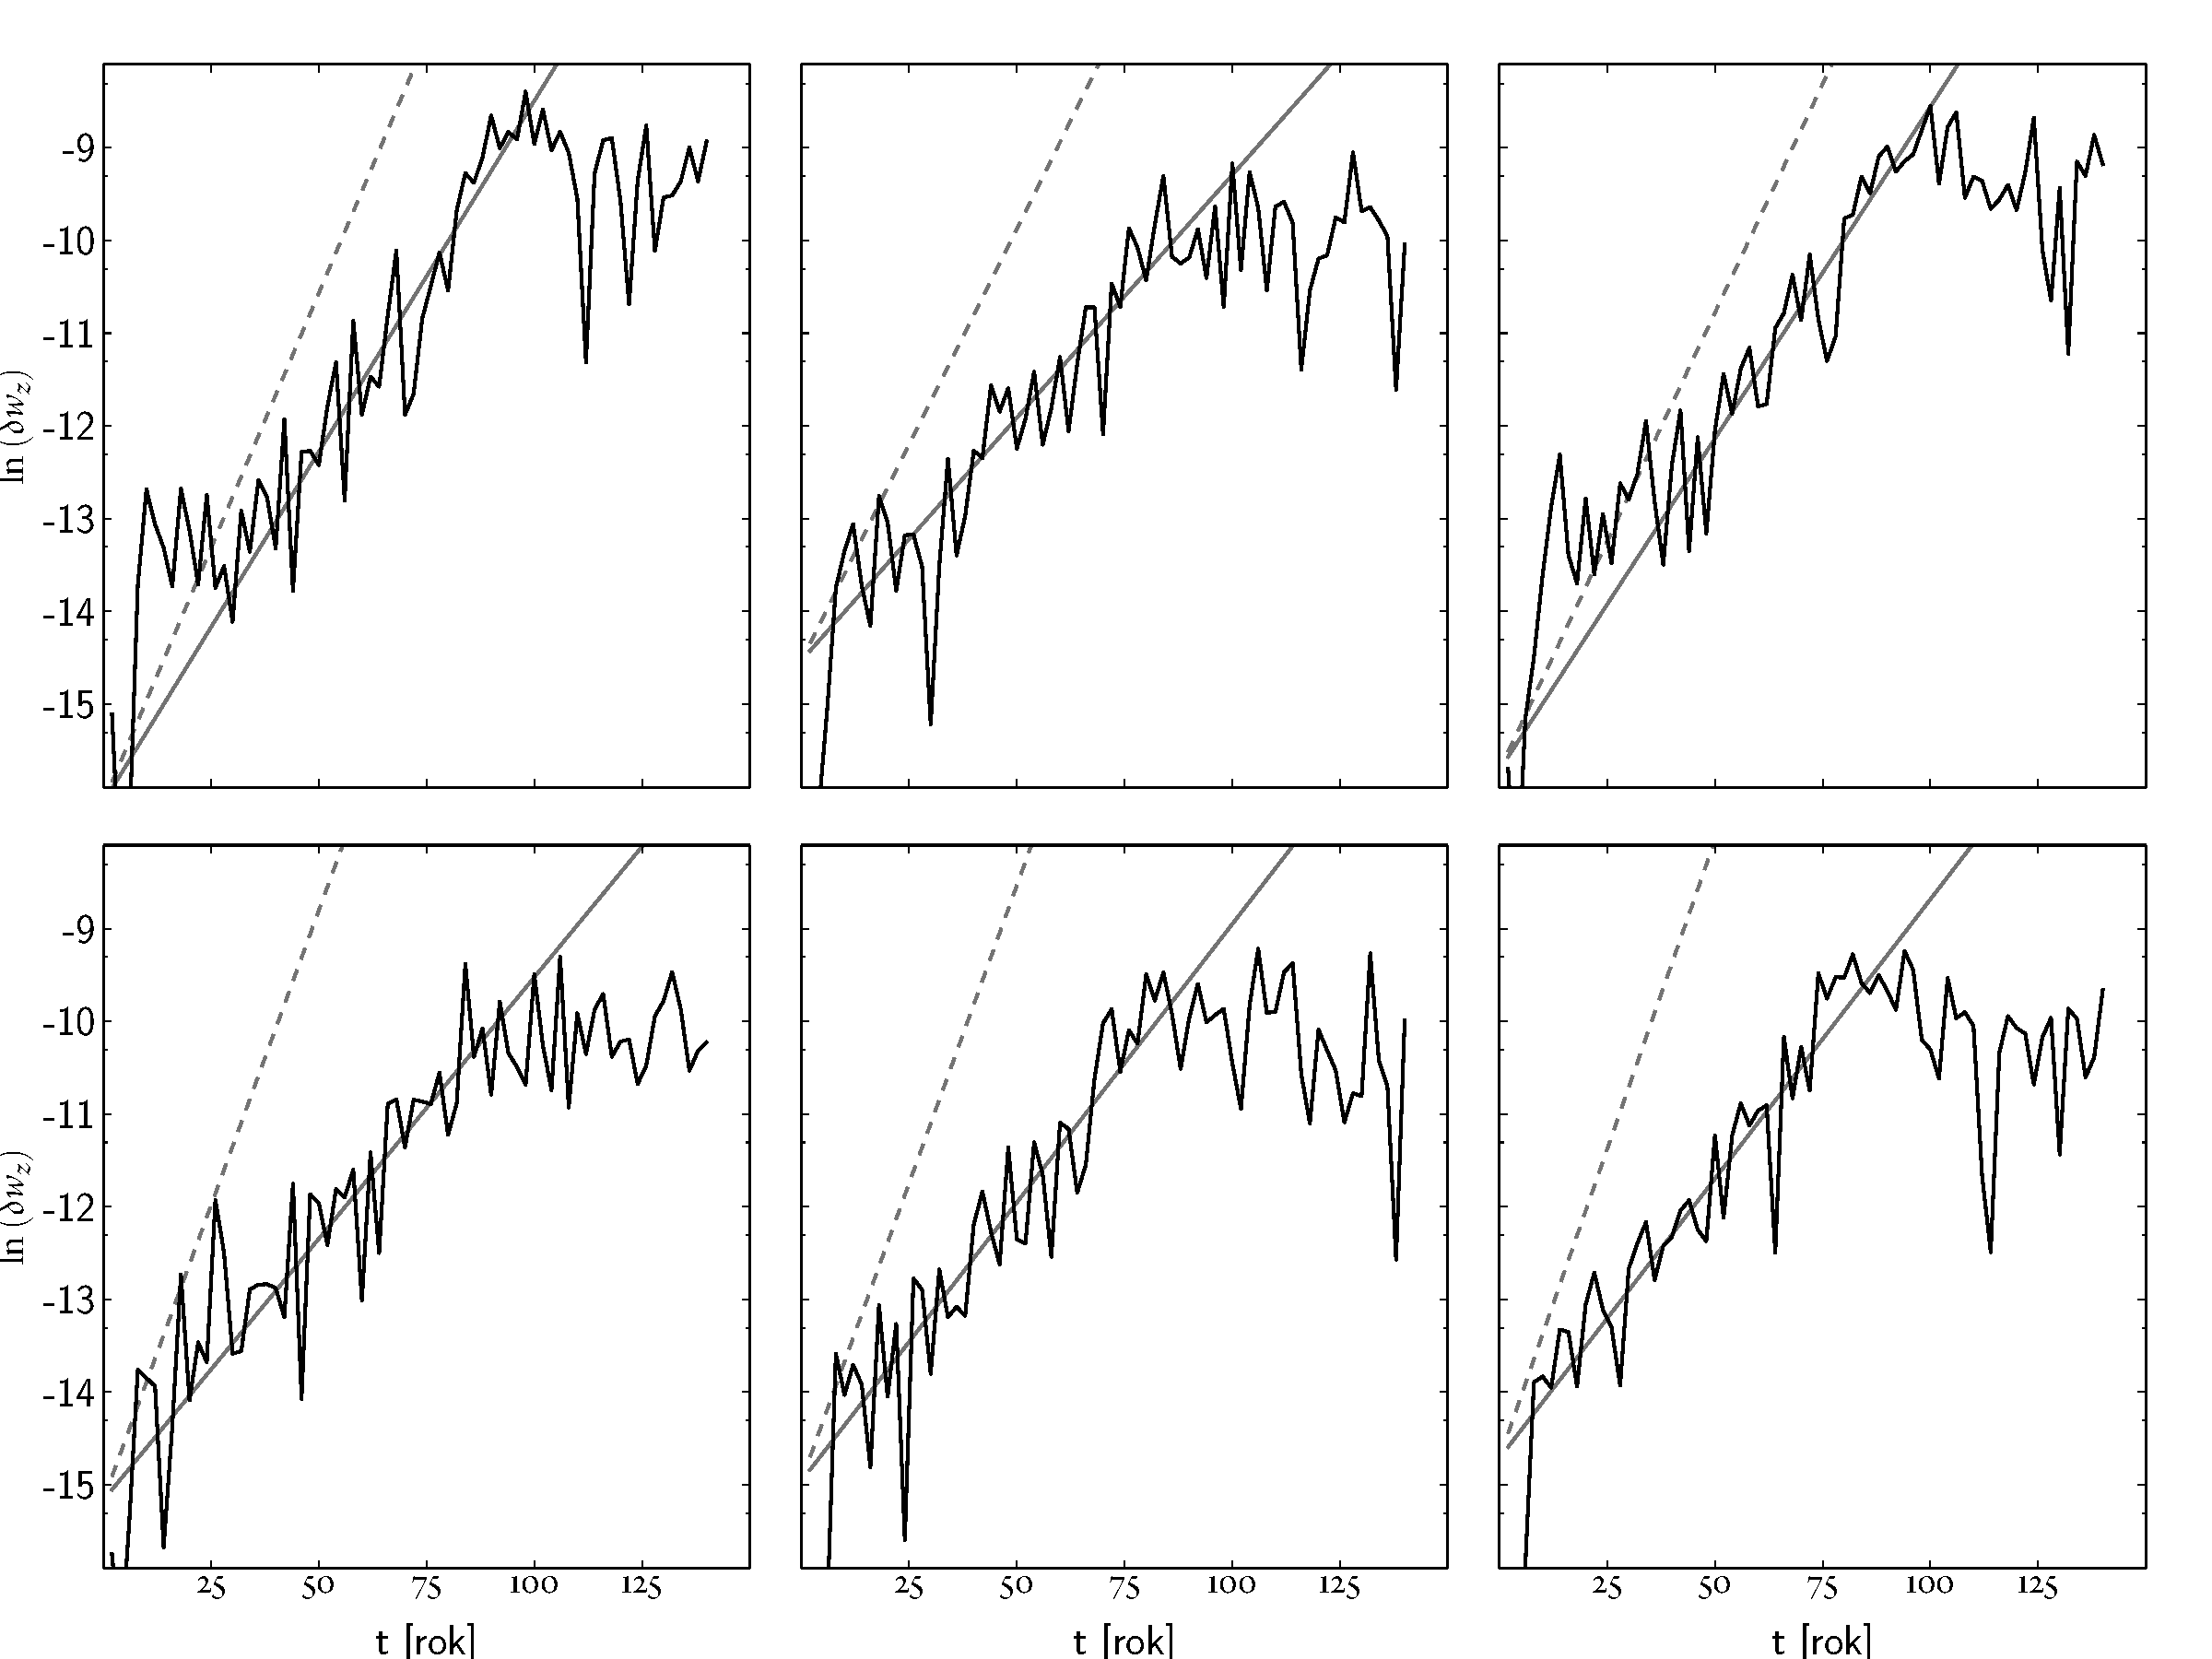
\includegraphics[height=0.44\textheight]{figures/sg_vlzd_growth}
   \caption{Czasowa ewolucja amplitud zaburzenia wertykalnej składowej prędkości
      pyłu (czarna krzywa) w~przestrzeni fourierowskiej dla łatki z~symulacji
      BD3d (6 górnych paneli) i BD3dS (6 dolnych paneli) obejmującej obszar
      $[3.35,3.65]\times[-0.15,0.15]~\AU^2$ dla $\varphi = \pi / 12$ wraz 
      z~dopasowaniem~\mref{eq:fit} (szara linia) i~przewidywanym tempem wzrostu
      wynikającym z~liniowej analizy stabilności (linia przerywana).}
   \label{fig:modes3d}
\end{figure}
%
\begin{figure}
   \centering
   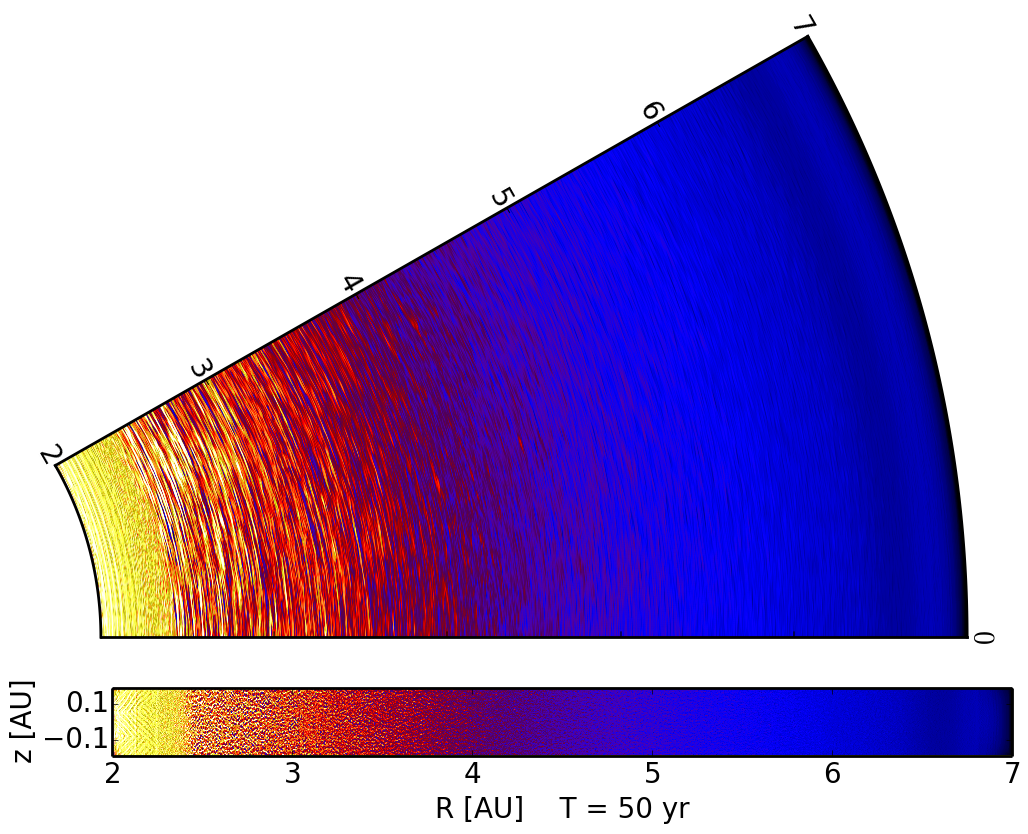
\includegraphics[width=0.44\linewidth]{figures/slice_sg_01}
   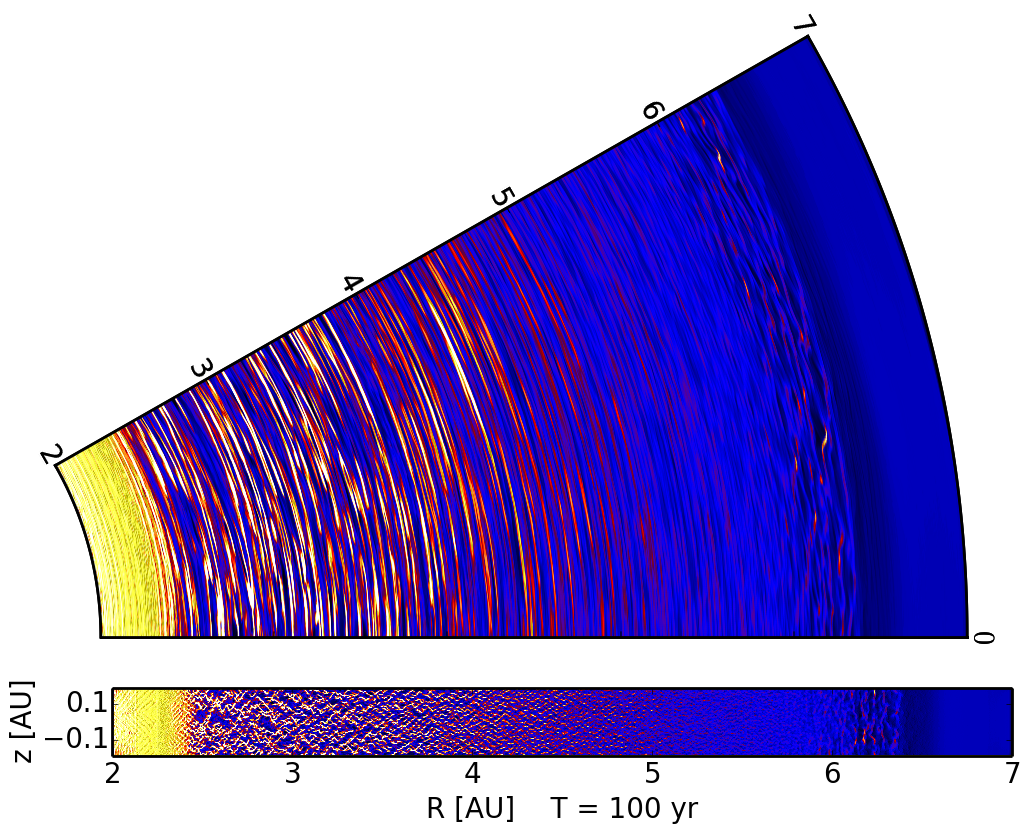
\includegraphics[width=0.44\linewidth]{figures/slice_sg_02} \\
   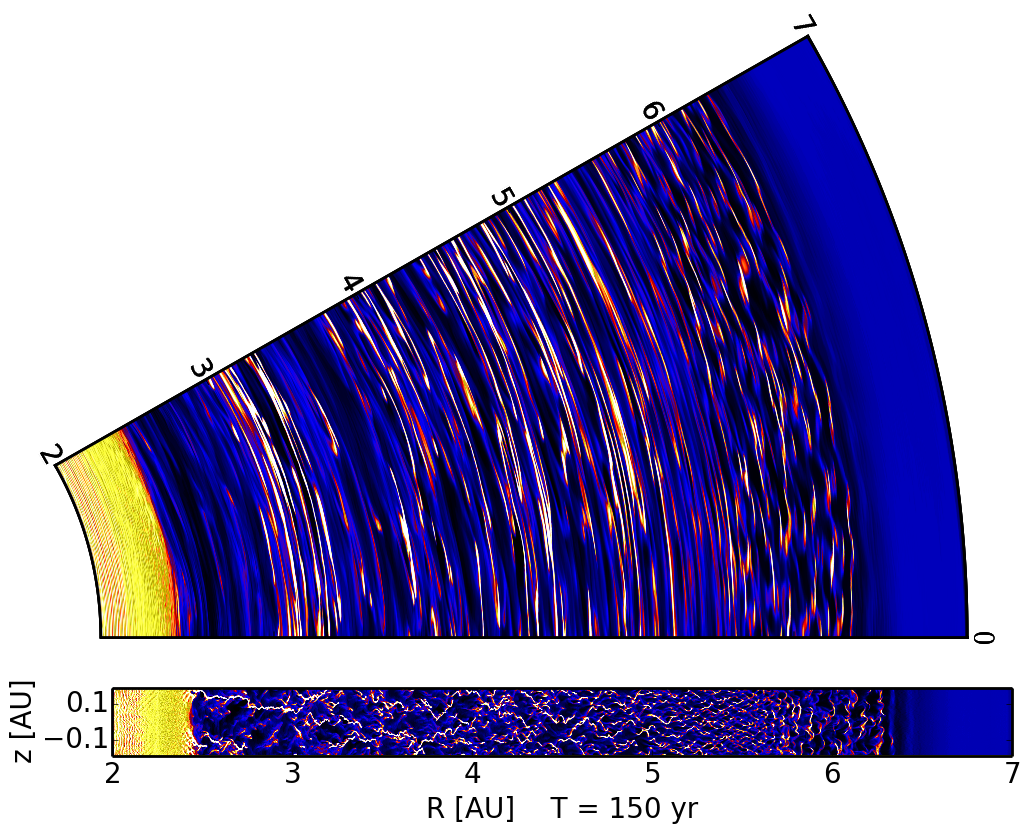
\includegraphics[width=0.44\linewidth]{figures/slice_sg_03}
   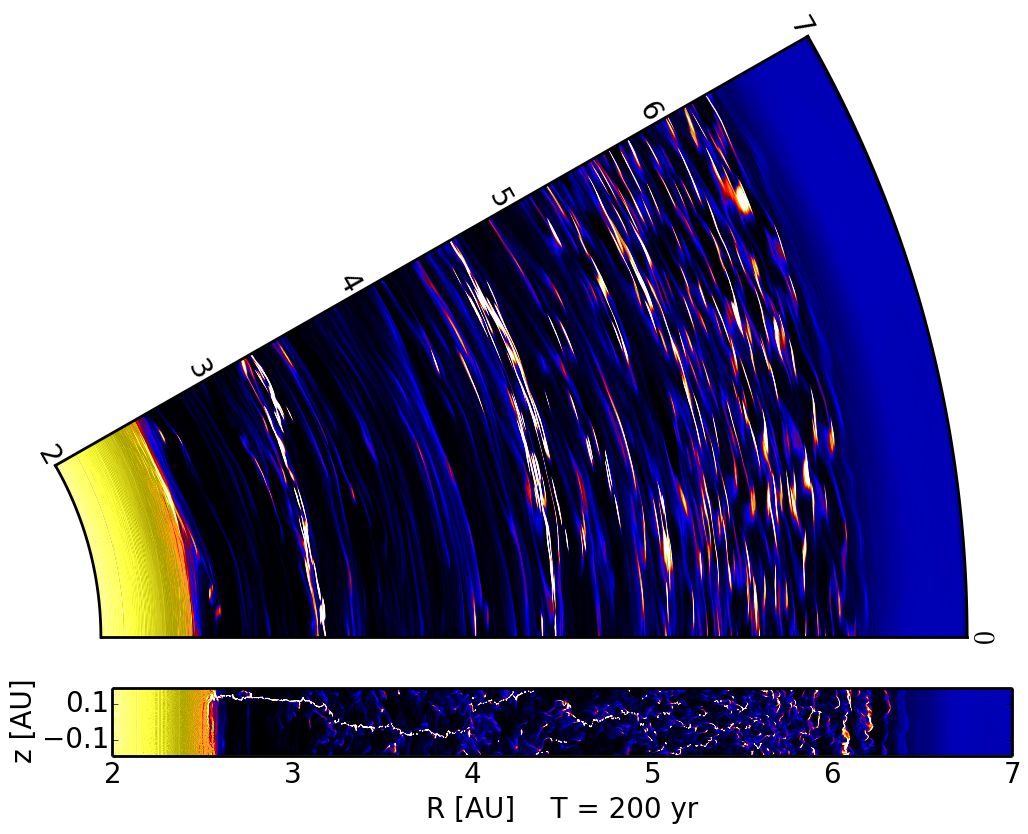
\includegraphics[width=0.44\linewidth]{figures/slice_sg_04} \\
   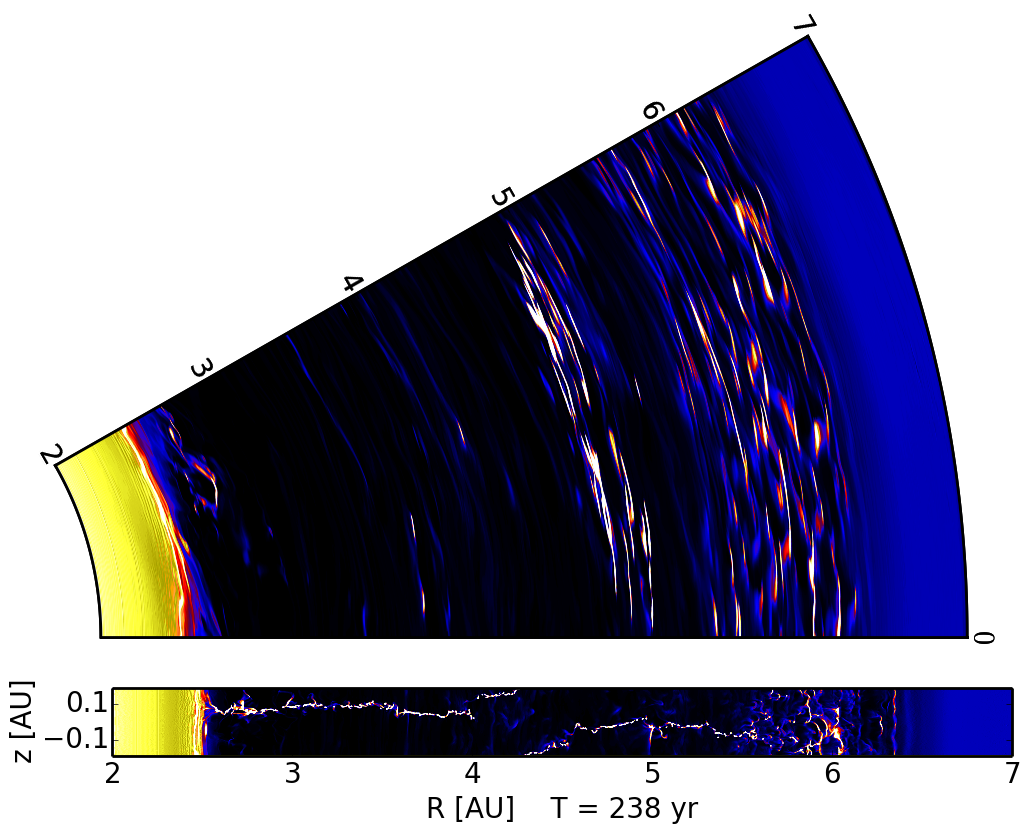
\includegraphics[width=0.44\linewidth]{figures/slice_sg_05}
   \caption{
      Migawki z~symulacji BD3dS obrazujące gęstość pyłu w~cięciach w
      płaszczyznach $R -\varphi$ oraz $R - z$ przechodzących przez środek 
   domeny obliczeniowej, dla czasów $T= 50, 100, 150, 200, 250$}
   \label{fig:slicesg}
\end{figure}
%
Pierwsza zauważalną różnicą jest przekroczenie przez pył gęstości na której
wcześniej niestabilność strumieniowa się wysycała (por. środkowy panel na
Rysunku~\ref{fig:hists}). Jest to prostą konsekwencją faktu, że każde formujące
się zagęszczenie jest dodatkowo ściskane działającą do wewnątrz siłą
samograwitacyjną. Po $150$~latach dysk pyłowy staje się widocznie bardziej
pofragmentowany w~kierunku azymutalnym w porównaniu z modelem bez
samograwitacji.  Odstępstwo od osiowej symetrii jest wyraźnie zauważalne.
Formacje gęstego pyłu na skutek wzajemnego oddziaływania grawitacyjnego (jak
i~własnego ciężaru) zaczynają się deformować coraz silniej zmieniając swoją
strukturę w~kierunku azymutalnym. W~ciągu kolejnych $50$~latach samograwitacja
,,ściska'' praktycznie cały pył do jednej płaskiej warstwy w~płaszczyźnie $R -
\varphi$ tworząc długie, pofalowane włókna (Rysunek~\ref{fig:projs}). W~trakcie
dalszej ewolucji włókna fragmentują na mniejsze związane grawitacyjnie obiekty,
które podlegają dalszym oddziaływaniom dynamicznym. 
%
\begin{figure}
   \centering
   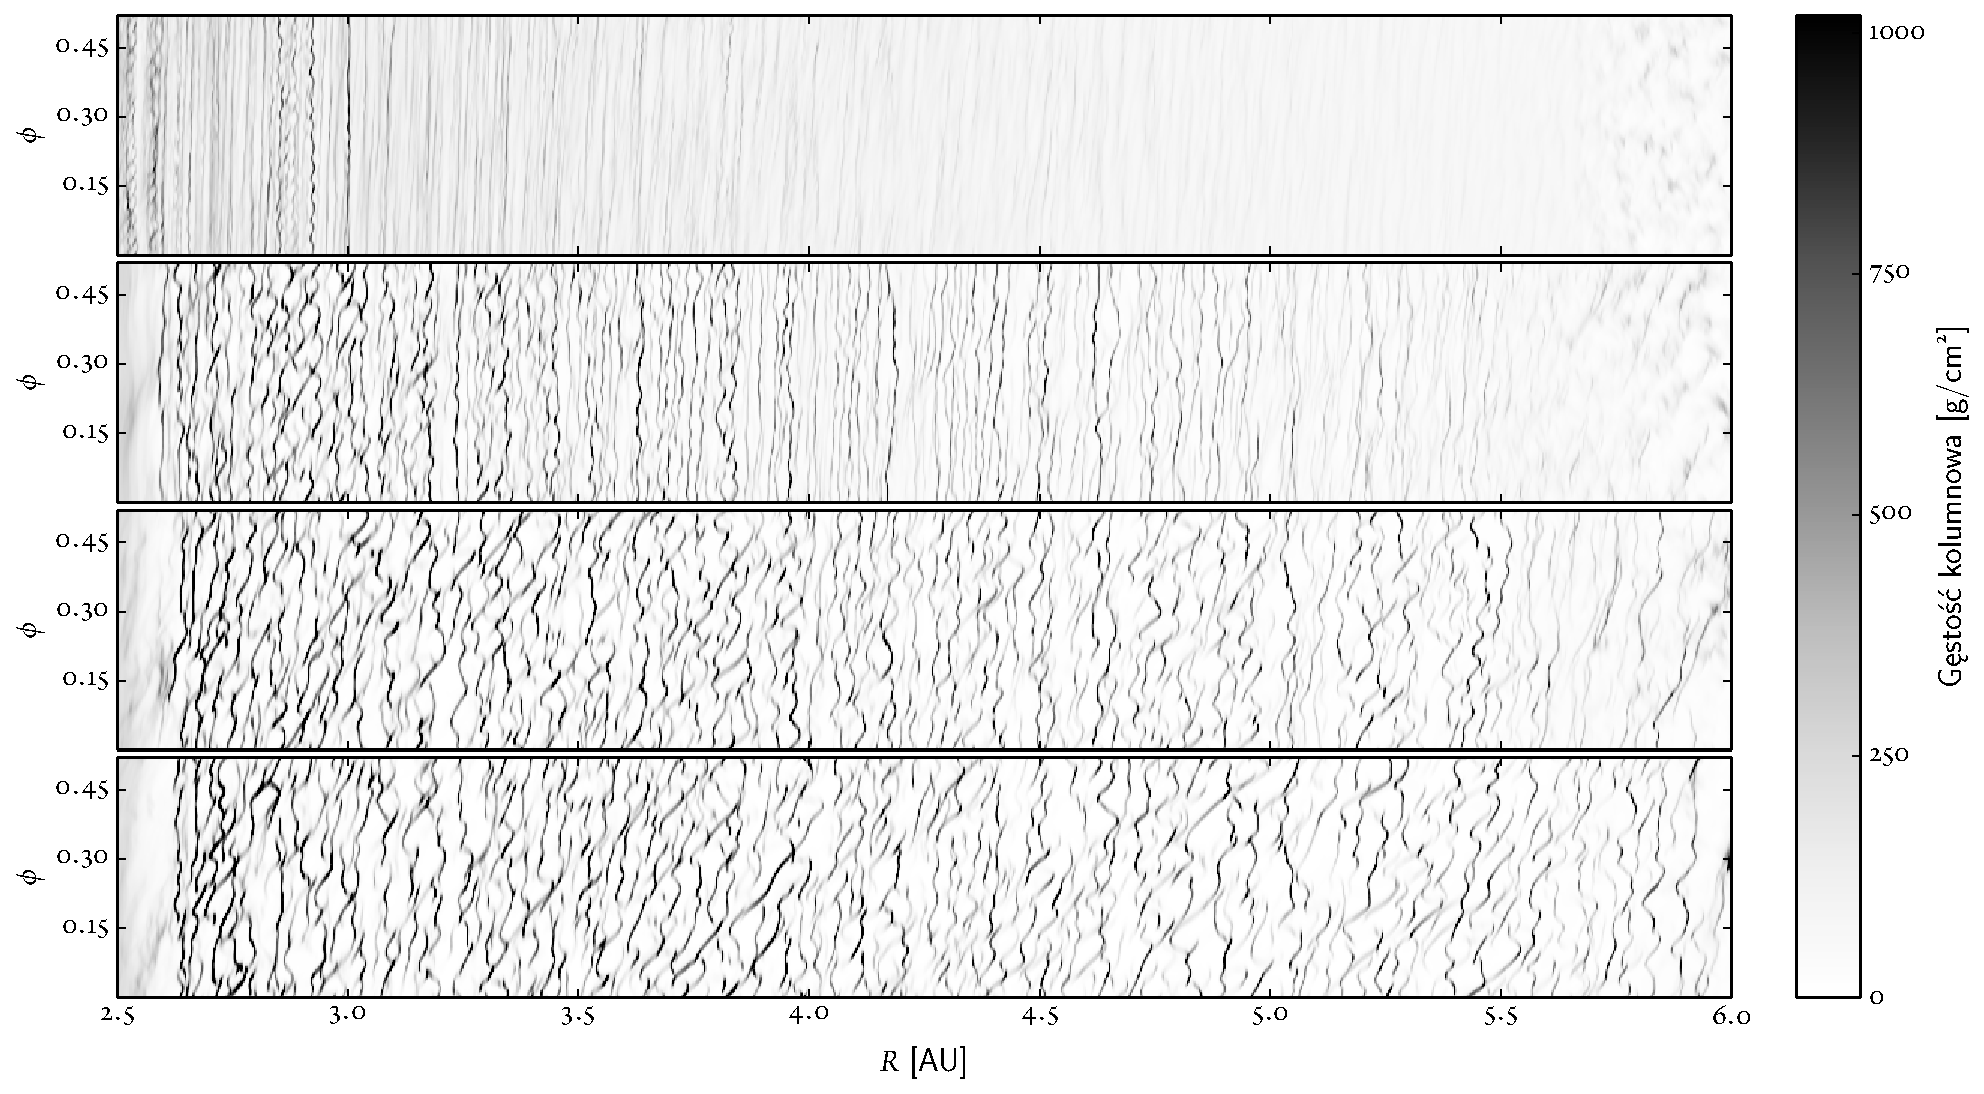
\includegraphics[width=0.95\linewidth]{figures/proj_sg}
   \caption{Gęstość kolumnowa pyłu w~symulacji BD3dS dla czasu $T=150, 200, 250, 300\yr$}
   \label{fig:projs}
\end{figure}
%
\begin{figure} 
  \centering
  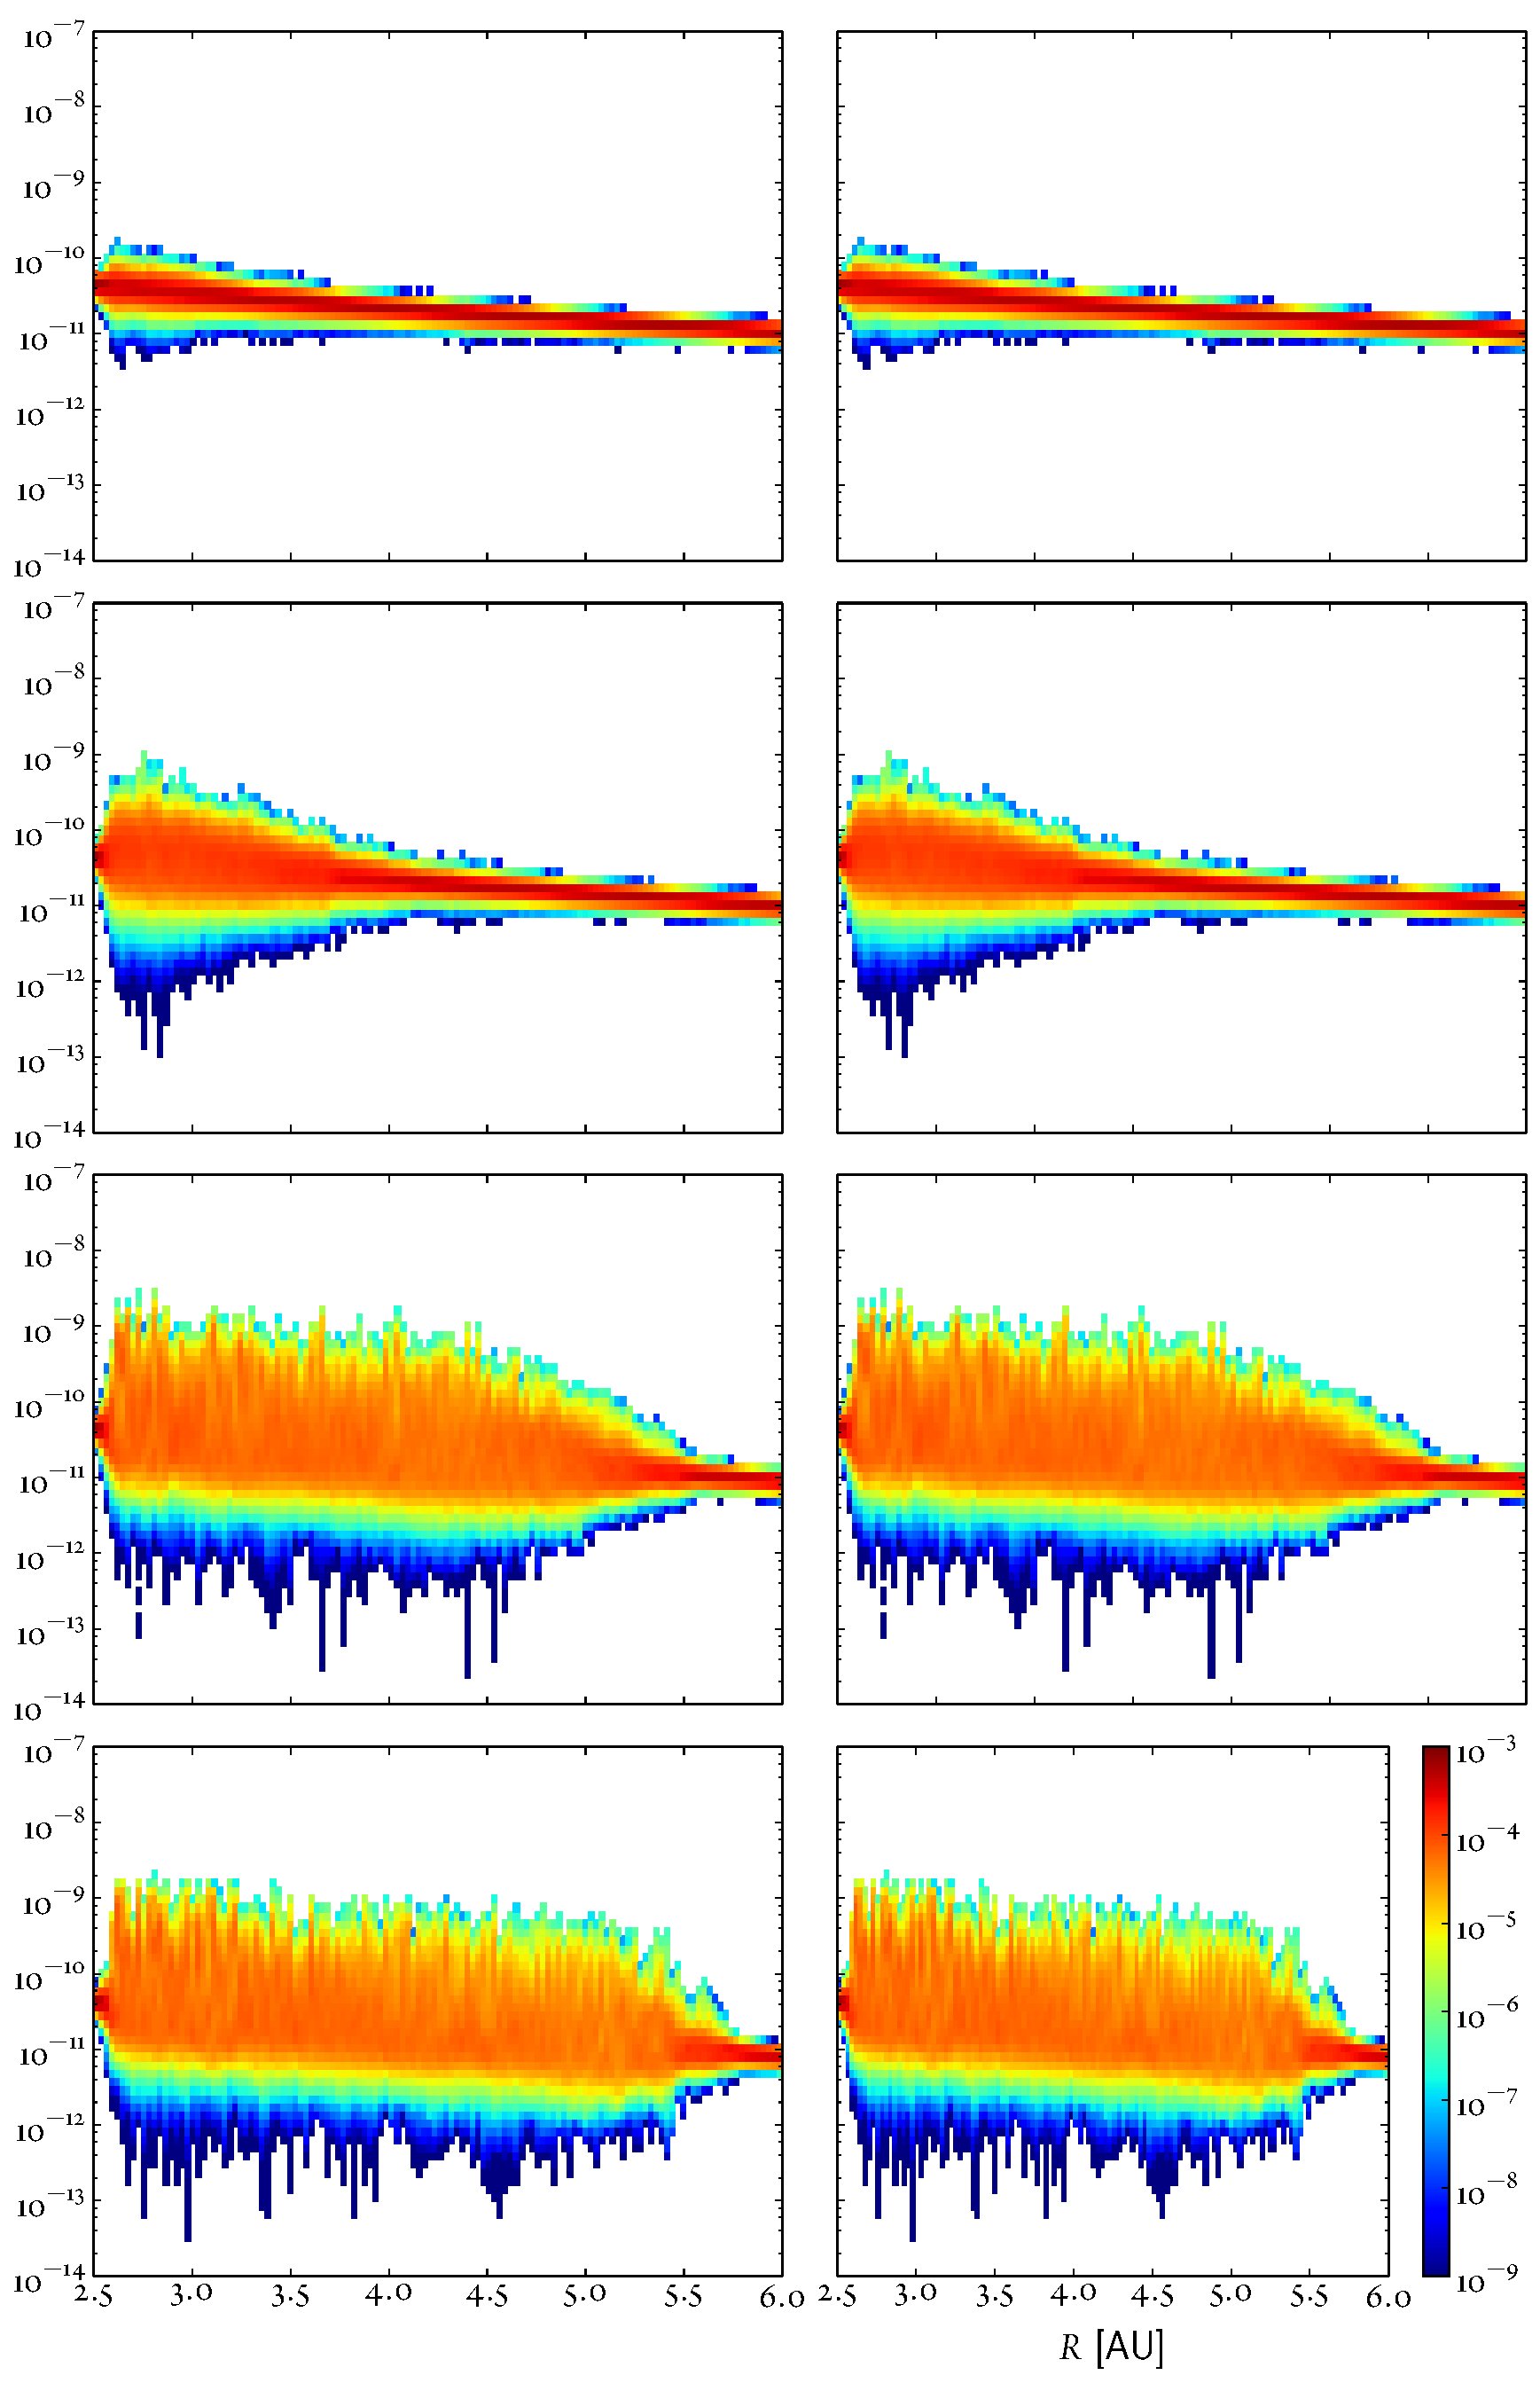
\includegraphics[height=0.9\textheight]{figures/hists2d}
  \caption{Histogramy masy pyłu w~funkcji promienia i~gęstości pyłu, lewa
  kolumna bez samograwitacji, prawa kolumna z~samograwitacja}
  \label{fig:hists} 
\end{figure}
%
Wpływ samograwitacji na ewolucję układu dobrze obrazuje zestawienie
histogramów masy pyłu w~funkcji promienia orbitalnego i~gęstości pyłu
(Rysunek~\ref{fig:hists}). Dla symulacji BD3d, pomimo osiągnięcia przez nią
lokalnie zagęszczeń o $1\div1.5$ rzędów większych niż początkowy rozkład,
większość masy pyłu jest równomiernie rozłożona pomiędzy gęstościami $10^{-11}
\div 5\cdot10^{-10}\g\cm^{-3}$. W~połączeniu obrazem wyłaniającym się
z~obserwacji wzbudzonych na rysunku zagęszczeń pyłowych, sugeruje to krótki czas
życia zagęszczeń i nieustający przepływ masy pomiędzy obszarami o niskiej
i~wysokiej gęstości.  Natomiast w~symulacji BD3dS rozkład masy jest zgoła inny.
Po osiągnięciu granicznej wartości gęstości $\sim10^{-9}\g\cm^{-3}$ masa zaczyna
przemieszczać się na histogramie w kierunku rosnących gęstości. Dla ustalonej
orbity, większość pyłu ostatecznie lokuje się w przedziale gęstości
$\sim10^{-8}\div10^{-9}\g\cm^{-3}$.  Wysycenie wzrostu zagęszczeń na poziomie
$10^{-8}\g\cm^{-3}$ jest najprawdopodobniej konsekwencją
ograniczonej rozdzielczości siatki obliczeniowej. W rzeczywistym świecie, wobec
braku własnego ciśnienia termicznego zagęszczenia pyłu powinny zapadać się do
momentu całkowitego sprasowania pyłu do postaci zwartych planetezymali. {\bf to
nie jest do końca prawdziwa teza}
\par Histogram masy niestety nie daję informacji o kształcie i
charakterystycznych rozmiarach obiektów w~których znajduje się większość masy pyłu,
ani nie pozwala stwierdzić czy pył jest grawitacyjnie związany. W~celu
rozszerzenia przeprowadzonej analizy zebrany materiał poddano procedurze
identyfikacji topologicznie powiązanych ze sobą komórek obliczeniowych, które
zawierają porcje pyłu o~gęstości w~przedziale $10^{-10}\div10^{-8}\g\cm^{-3}$. W~tym
celu wykorzystano pakiet do analizy i~wizualizacji
danych~\yt{}~\footnote{Szczegółowe informacje na temat \emph{clump-finder'a}
można znaleźć w~rozdziale 7.7 w~pracy~\cite{yt}. Autor niniejszej pracy
rozszerzył pakiet \yt{} o możliwość czytania plików wynikowych z~kodu
PIERNIK, a także zaimplementował wsparcie dla współrzędnych cylindrycznych.}.
Uzyskanie informacji o strukturze rozkładu gęstości pyłu jest pierwszym krokiem w
celu ustalenia, czy powstające zagęszczenia są w~stanie utworzyć grawitacyjnie
związane obiekty. Dla każdego zidentyfikowanego obiektu można
określić relację pomiędzy jego energią kinetyczną i energia potencjalna
w układzie związanym ze środkiem masy obiektu. Uznajemy, że obiekt jest
grawitacyjnie związany, gdy energia kinetyczna jest mniejsza od głębokości
lokalnej studni potencjału:
%
\begin{equation}
   \label{eq:bcrit}
   E_{\textrm{kin}} \equiv \sum\limits_{i=1}^N \frac{m_i\tilde{\mathbf{v}}_i^2}{2} 
   < \sum\limits_{i=1}^N m_i\tilde{\Phi}_i \equiv E_{\textrm{pot}},
\end{equation}
%
gdzie $N$ to liczba komórek obliczeniowych wypełnionych przez pył tworzący
obiekt, $m_i$, $\tilde{\mathbf{v}}$, $\Phi_i$ to odpowiednio masa pyłu, prędkość
w~układzie środka masy obiektu, potencjał w centrum wybranej komórki. Potencjał
samograwitacyjny został uzyskany bezpośrednio z~PIERNIKa jako rozwiązanie
równania Poissona~\mref{eq:poisson} dla sumarycznej gęstości obu składników
płynowych (gazu i pyłu).  Lokalne zagłębienia potencjału grawitacyjnego w
otoczeniu badanych obiektów pyłowych można obliczyć, poprzez odjęcie potencjału
grawitacyjnego uśrednionego w płaszczyźnie \emph{z-$\varphi$} dla zadanego
promienia $R$:
%
\begin{equation}
   \tilde{\Phi}_i(R,\varphi,z) = \Phi_i(R,\varphi,z) -
   \left<\Phi_i\right>_{z\varphi}(R).
\end{equation}
%
Przy obliczaniu energii kinetycznej obiektu wykonywana jest transformacją
współrzędnych do układu środka masy, w~celu uwzględnienia wpływu rotacji.
Jest to niezbędne, ponieważ siła odśrodkowa przeciwdziała kontrakcji obłoku na
skutek samograwitacji. Aby uniknąć przeszacowania ilości materii, która zostaje
związana grawitacyjnie dodatkowo wzięto pod uwagę możliwy wpływ turbulencji
zachodzącej w skalach przestrzennych poniżej zdolności rozdzielczej siatki
obliczeniowej. Do opisu podskalowej turbulencji użyto klasycznej parametryzacji
współczynnikiem $\alpha$~\cite{SS73}. Ostateczna postać energii kinetycznej
obiektu jest wyrażona poprzez:
%
\begin{equation}
   \label{eq:ekin}
   \tilde{\mathbf{v}}_i = \mathbf{v}_i - \frac{\sum m_i \mathbf{v}_i}{\sum m_i}
   + \alpha c_s^2,
\end{equation}
%
gdzie wartość $\alpha$ ustalono na $0.01 \div 0.1$. Zastosowanie
kryterium~\mref{eq:bcrit} dla każdego zidentyfikowanego obiektu, pozwoliło na
określenie jaka część masy została skupiona w grawitacyjnie związanych
obiektach. Zależność ilości masy pyłu związanego grawitacyjnie w funkcji czasu
oraz parametru $\alpha$ przedstawiono na lewym panelu rysunku~\ref{fig:bmasstime}.
%
\begin{figure}[ht]
  \centering
  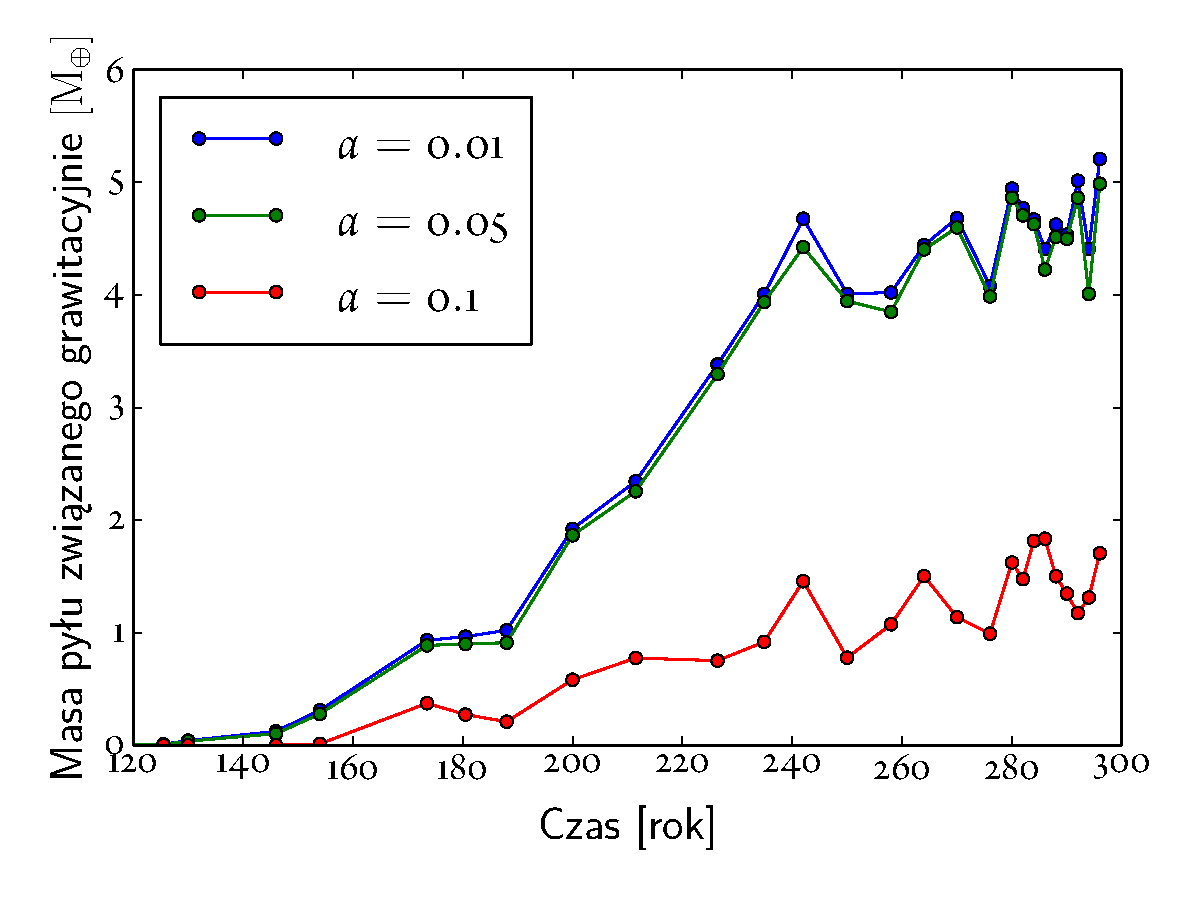
\includegraphics[width=0.45\textwidth]{figures/bmass_vs_time}
  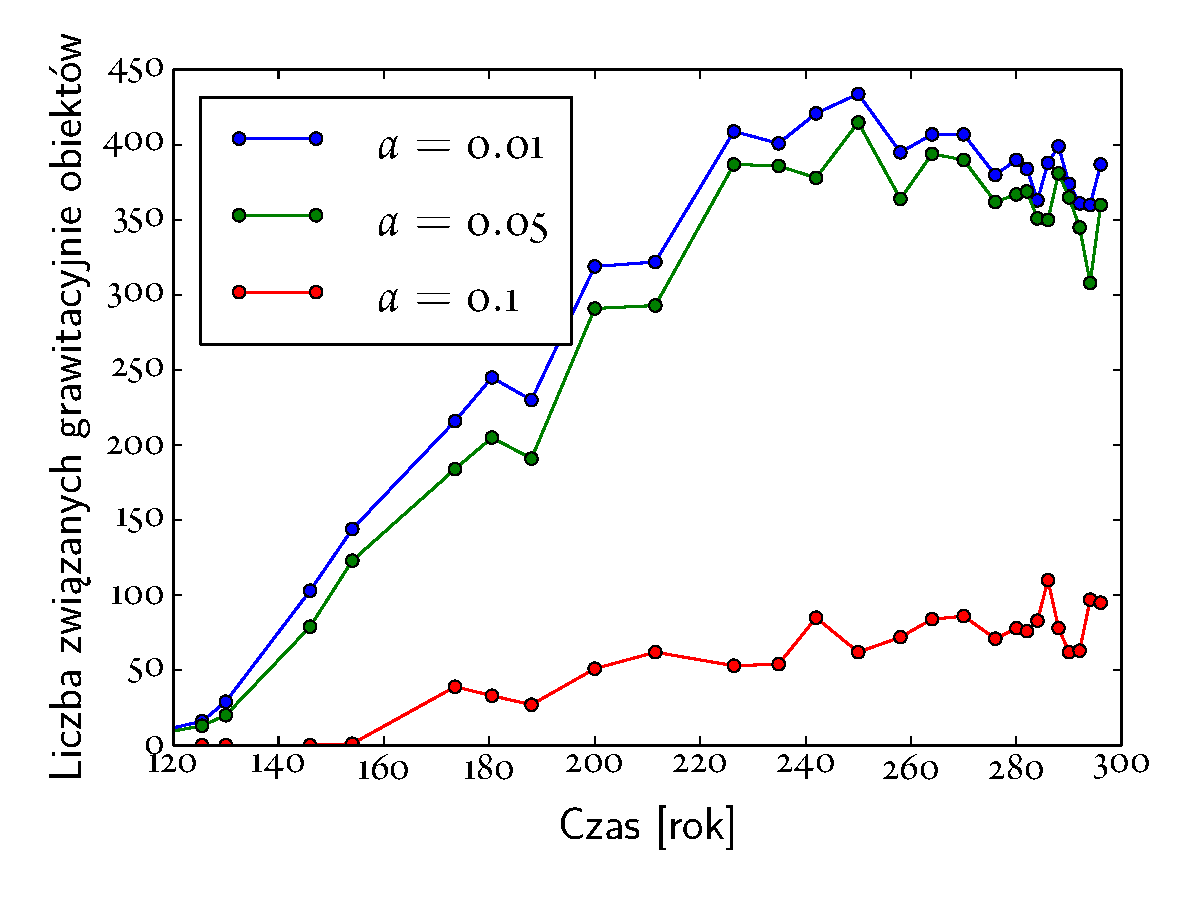
\includegraphics[width=0.45\textwidth]{figures/nclumps_vs_time}
  \caption{Lewy panel przedstawia ilość masy pyłu, która według
     kryterium~\mref{eq:bcrit} została zgromadzona w grawitacyjnie związanych
     obiektach w funkcji czasu. Wartość maksymalna osiągnięta po około 300
     latach ($4\div5\Mearth$ dla $\alpha = 0.05$) stanowi około $13\div14\%$
     całkowitej masy pyłu, Prawy panel przedstawia ilość grawitacyjnie
     związanych obiektów w funkcji czasu i parametru $\alpha$ znalezionych przy
     pomocy procedury opisanej w niniejszym rozdziale.}
  \label{fig:bmasstime} 
\end{figure}
%
%
Na ostateczną masę pyłu zgromadzoną w związanych obłokach i ich liczbę, duży
wpływ ma wartość parametru $\alpha$. Pierwsze związane obiekty pojawiają się po
około 120 latach od momentu rozpoczęcia symulacji. Pod czas kolejnych
$100\div120$ lat następuje intensywny wzrost wartości masy zgromadzonej w
związanych obiektach. Dla $\alpha = 0.05$, po czasie około $T = 250$~lat masa
pyłu związana w samograwitujących obłokach stabilizuje się na poziomie $14\%$
całkowitej masy pyłu. Dla $\alpha = 0.1$ maksymalna masa zgromadzona w obłokach
oscyluje wokół $5\%$ masy całkowitej. Dla $\alpha < 0.05$ wyraz wynikający
z~turbulentnego transportu momentu pędu staje się zaniedbywalny i~nie zmienia
znacząco liczby związanych obłoków pyłu. Liczba grawitacyjnie związanych
obiektów w funkcji czasu i parametru $\alpha$ została przedstawiona na prawym
panelu rysunku~\ref{fig:bmasstime}. W okresie $120 \div 220$~lat, dla $\alpha
\leq 0.05$ następuje liniowy wzrost liczby związanych obiektów w tempie około 40
obiektów na 10 lat, aż do osiągnięcia granicznej wartości ok. $380$ obiektów dla
$T > 240$~lat co stanowi $40\%$ z liczby wszystkich obiektów znalezionych przy
pomocy ,,clump-findera''. Dla $\alpha = 0.1$ wzrost liczby obiektów następuje w tempie
około 5 obiektów na 10 lat i nie można mówić o jego wysyceniu w trakcie czasu
trwania symulacji. W tym wypadku maksymalna liczba pod koniec czasu trwania
symulacji wynosi około $100$, co stanowi około $10\%$ wszystkich obiektów
znalezionych przy pomocy procedury opisanej w tym rozdziale.
%
\begin{figure}[ht]
   \centering
   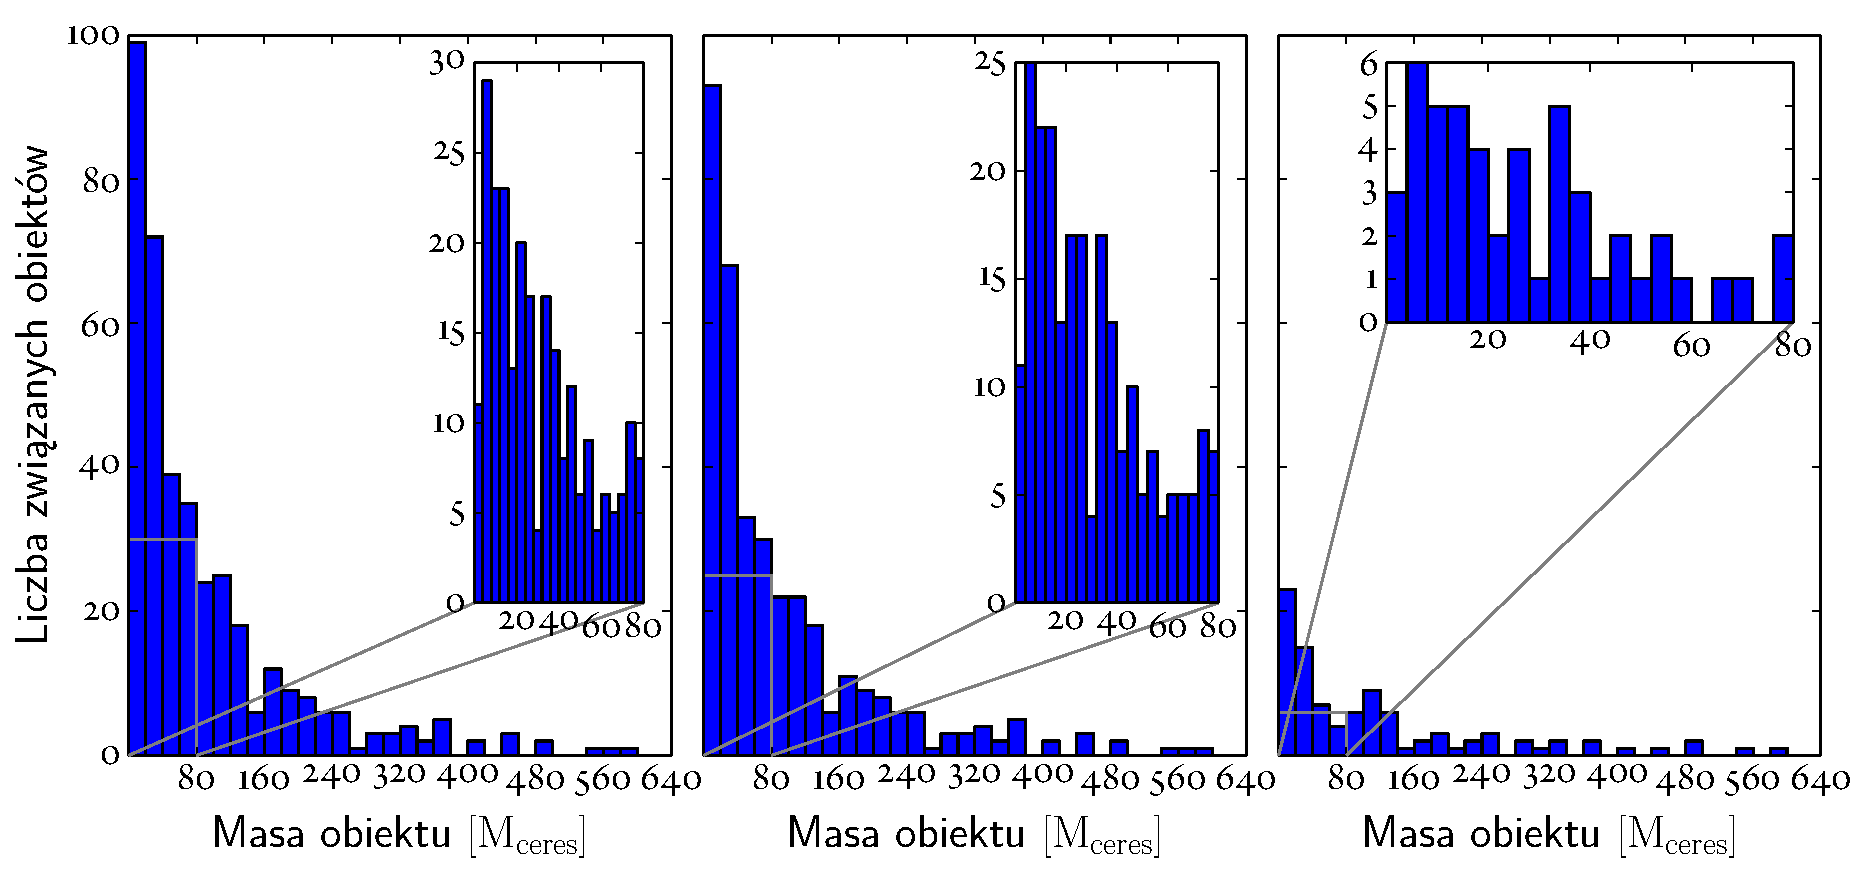
\includegraphics[width=0.95\linewidth]{figures/mass_hists}
   \caption{Histogramy masy obiektów związanych dla $\alpha = 0.01, 0.05, 0.1$
   (odpowiednio panel lewy, środkowy i prawy) w zakresie $[0,600]\Mceres$.
   Szerokość pojedynczego przedziału wynosi $20\Mceres$. Na wewnętrznych
   panelach znajdują się histogramy dla obiektów o masach mniejszych niż
   $80\Mceres$. Szerokość pojedynczego przedziału na wewnętrznym panelu wynosi
   $4\Mceres$}
   \label{fig:masshist}
\end{figure}
%
\par Szczegółowy histogram mas wszystkich zidentyfikowanych obiektów dla czasu
$T=300$~lat i parametru $\alpha = 0.01, 0.05, 0.1$ został przedstawiony na
Rysunku~\ref{fig:masshist}. Bez względu na wartość parametru $\alpha$ ponad
$25\%$ obiektów związanych grawitacyjnie ma masę mniejszą niż
$20\Mceres$~\footnote{Masa Ceres wynosi około $9\cdot10^{23}\g$ co stanowi około
$0.015\Mearth$}, przy czym najmniej masywny obiekt ma nieco ponad $2.5\Mceres$.
Dla zakresu mas od $0$ do $40\Mceres$ liczba obiektów związanych przekracza
$40\%$ liczby wszystkich obiektów. Zaledwie $50$ obiektów dla $\alpha \leq
0.05$ oraz $20$ obiektów dla $\alpha = 0.1$ przekracza masę $200\Mceres$.
Najmasywniejszy z nich osiąga masę $600\Mceres$.
%
\par Złożenie histogramów masy obiektów dla czasu od 250 do 300 lat
przedstawione na rysunku~\ref{fig:massfun} pozwala oszacować funkcję masy
samograwitacyjnie związanych obiektów, która może być interpretowana jako
początkowa funkcja masy dla przyszłych planetezymali formujących się w toku
dalszej ewolucji układu. Na przedziale $[40, 300]\Mceres$ przebieg funkcji masy
obiektów związanych grawitacyjnie można przybliżyć funkcją potęgową o wykładniku
$-5/4$. Obiekty o masach mniejszych niż $40\Mceres$ są reprezentowane w
symulacji przez co najwyżej kilkadziesiąt komórek obliczeniowych, co przekłada
się na ich liniowy rozmiar rzędu kilku komórek. Tak niewielka ilość komórek
obliczeniowych przekłada się na znaczną niepewność w dokładności obliczenia
siły wynikającej z samograwitacji w danym obiekcie. Należy zatem przyjąć, iż
liczba obiektów w tym przedziale masy i rozmiarów liniowych jest mocno
niedoszacowana. Z kolei dla przedziału mas większych niż $300\Mceres$, mamy
do czynienia z pojedynczymi obiektami, przez co próbka jest statystycznie
niereprezentatywna.
%
\begin{figure}[ht]
   \centering
   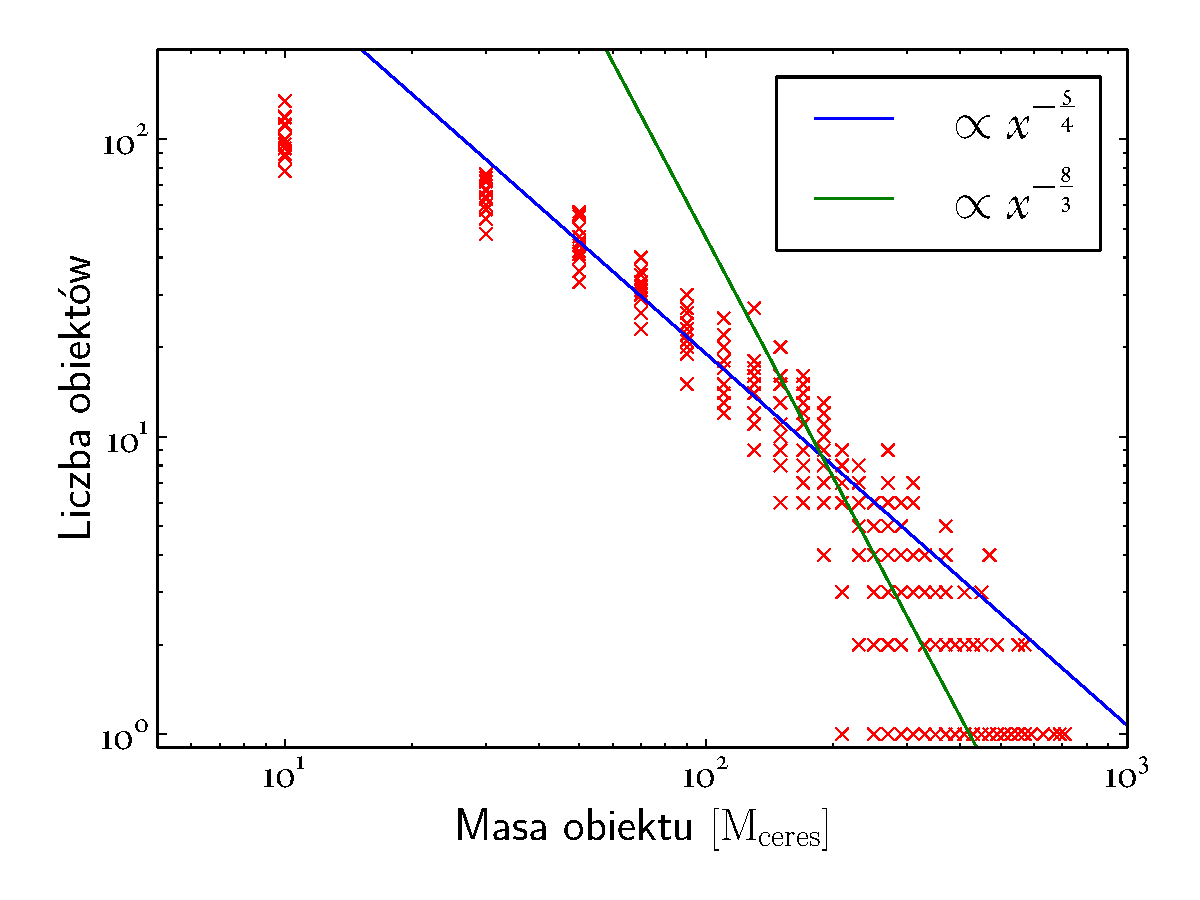
\includegraphics[width=0.7\linewidth]{figures/mass_func}
   \caption{Złożenie histogramów masy obiektów związanych grawitacyjnie dla
   $\alpha = 0.05$ dla $T \in [250, 300]$ lat (czerwone punkty). Niebieska linia
stanowi dopasowanie funkcji wykładniczej do liczby obiektów w funkcji masy na
przedziale $[40,200]\Mceres$. Zielona linia przedstawia schematycznie funkcję
wykładniczą o wykładniku $-8/3$ odpowiadającą funkcji początkowej funkcji mas
planetezymali przedstawionej w pracy~\cite{MFFK98}}
   \label{fig:massfun}
\end{figure}
%
\par W niniejszym rozdziale przedstawiono wyniki trójwymiarowych symulacji
dwuskładnikowego (gaz i pył) dysku protoplanetarnego z uwzględnieniem
samograwitacji. W szczególności wskazano, że taki układ dzięki połączeniu
niestabilności strumieniowej i niestabilności grawitacyjnej może wytworzyć
grawitacyjnie związane obiekty składające się z pyłu o masach odpowiadających
planetezymalom o rozmiarach rzędu setek kilometrów, przy założeniu iż cała masa
pyłu uformowałaby zwarte ciało. Szczegółowa dyskusja wyników takich jak funkcja
masy otrzymanych związanych samograwitacyjnie obiektów w kontekście ich dalszej
ewolucji zostanie przedstawiona w następnym rozdziale.
%
%\begin{itemize}
%   \item Potrzebna jest szczegołowa dyskusja histogramu na rys. 4.3.5
%      \note[KK]{usunięty na rzecz rys.~\ref{fig:masshist}, szczegółowa dyskusja
%      w tekście}
%   \item ile powstało obiektów? \note[KK]{Rysunek~\ref{fig:bmasstime} i
%      dyskusja w tekście}
%   \item jaki jest zakres mas i ewentualnie funkcja masy?
%      \note[KK]{Rysunek~\ref{fig:massfun} i dyskusja w tekście}
%   \item jaka jest całkowita masa skupiona w obiektach związanych grawitacyjnie?
%      \note[KK]{Rysunek~\ref{fig:bmasstime} i dyskusja w tekście}
%   \item jakie jest tempo wyłapywania masy pyłu przez obiekty związane?
%      \note[KK]{Nie bardzo jest jak to określić}
%   \item jaki jest rozkład masy obiektów związanych w funkcji $R$? \note[KK]{z
%      tego rezygnujemy, bo nic ciekawego nie widać}
%   \item jak te wyniki mają się do Układu Słonecznego? \note[KK]{będzie w
%      rozdziale 5}
%\end{itemize}
%
%\begin{figure}
%   \centering
%   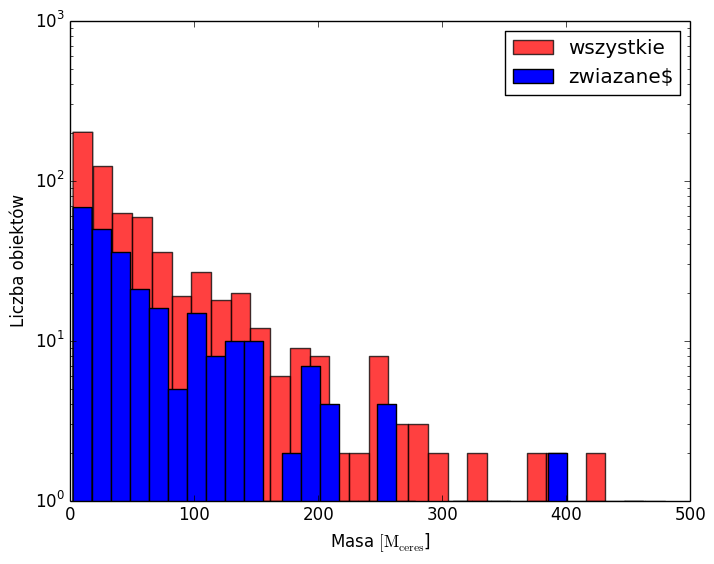
\includegraphics[width=0.49\linewidth]{figures/masshist.png}
%   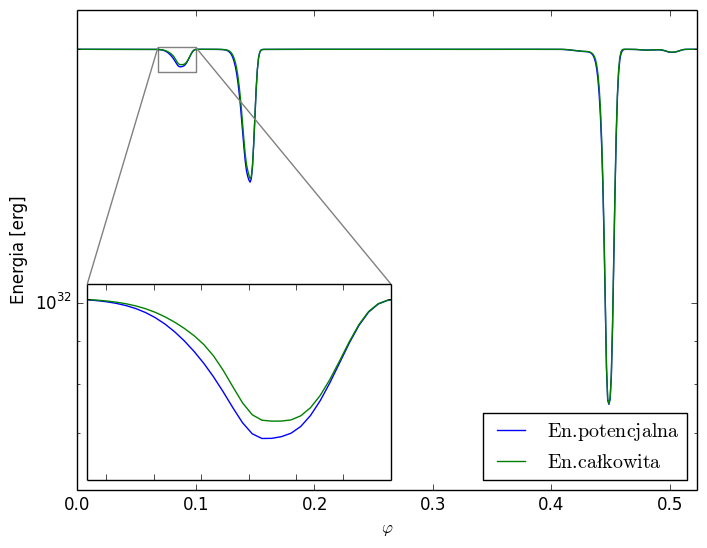
\includegraphics[width=0.49\linewidth]{figures/energie.png}
%   \caption{(Lewy panel) Histogram przedstawiający rozkład masy w~topologicznie powiązanych
%   obiektach istniejących w~domenie obliczeniowej dla symulacji BD3dS dla czasu
%   $T=250\yr$. Kolorem niebieskim zaznaczono clumpy związane grawitacyjnie, zaś
%   kolorem czerwonym wszystkie obiekty.
%   (Prawy panel) Przekrój azymutalny przez domenę obliczeniową dla $R=3.84\AU$
%   i~$z=0.01\AU$ dla czasu $T=250\yr$ pokazujący energię potencjalną (zgodnie z
%   definicją w~równaniu~\mref{eq:bcrit}) oraz sumę energii potencjalnej i~energii
%   kinetycznej dla danego clumpu.}
%   \label{fig:masshist_fail}
%\end{figure}
%
%   
% vim: tw=80 ts=3: 
